\documentclass[14pt]{extreport}
\usepackage[T2A]{fontenc}
\usepackage[utf8x]{inputenc}
\usepackage[english,russian]{babel}
\usepackage[T2A]{fontenc}
\usepackage[utf8x]{inputenc}
\usepackage[english,russian]{babel}
\usepackage{
  % cmap, % copy from pdf
  graphicx,
  subcaption,
  xcolor,
  caption,
  subcaption,
  hyperref, % for url in bibtex
  lineno,
  geometry,
  amssymb,
  amsfonts,
  amsmath, % for \begin{equation*}
  mathtext,
  cite,
  enumerate,
  float, % for figure with [ht]
  calc, % \widthof{999}
  amsthm
}
\usepackage{geometry}
\usepackage{lineno}

\newcommand{\bra}[1]{\left\langle #1 \right|}
\newcommand{\ket}[1]{\left| #1 \right\rangle}
\newcommand{\p}[1]{\left( #1 \right)}
\newcommand{\abs}[1]{\left| #1 \right|}
\newcommand{\tr}[1]{\mathrm{Tr} \left\{ #1 \right\}}
\newcommand{\sx}{I_\mathrm{x}}
\newcommand{\sy}{I_\mathrm{y}}
\newcommand{\sz}{I_\mathrm{z}}
\newcommand{\hdz}{H_\mathrm{dz}}
\newtheorem{definition}{Определение}[section]
\newtheorem{theorem}{Теорема}[section]


\graphicspath{{figures}}
\hypersetup{
  hidelinks, 
  unicode=true  % fix "PD1 encoding, removing `\CYRI'"
} 

% page margins
\geometry{left=25mm}
\geometry{right=10mm}
\geometry{top=20mm}
\geometry{bottom=20mm}
\linenumbers
\title{Многочастичная запутанность в многоквантовой спектроскопии ЯМР в твердом теле}
\author{Илья Лазарев}
\date{Последняя редакция: \today}

\begin{document}
\maketitle
\begin{titlepage}
\begin{flushright}
   Приложение № 5 \\
   к Положению о диссертационном \\
   совете Московского государственного \\
   университета имени М.В.Ломоносова
\end{flushright}
\vspace{1cm}
\begin{center}
  {\large Московский государственный университет им. М.В. Ломоносова} \\
  {\it Факультет фундаментальной физико-химической инженерии} \\
  \vspace{1cm}
  {\large Институт проблем химической физики РАН} \\
  {\it Лаборатория спиновой динамики и спинового компьютинга} \\
  \vfill
  (на правах рукописи) \\
  \vfill
  {\Large \bf Лазарев Илья Дмитриевич} \\
  \vspace{1cm}
  {\Large \bf
      Многочастичная запутанность \\
      в многоквантовой спектроскопии ЯМР \\
      \vspace{2mm}
      в твердом теле
  }
 \vfill
 01.04.07 Физика конденсированного состояния \\
 \vspace{1cm}
 ДИССЕРТАЦИЯ \\
 на соискание ученой степени \\
 кандидата физико-математических наук
 \vfill
 {\large
   Научный руководитель:\\
   д.ф.-м.н. профессор Фельдман Эдуард Беньямиович
 }
 \vfill
 Москва, 2022 г.
\end{center}
\end{titlepage}\addtocounter{page}{1}
\tableofcontents
\chapter*{Введение}
\addcontentsline{toc}{chapter}{Введение}

% Во введении к диссертации определяется актуальность избранной темы, степень ее разработанности, цели и задачи, объект и предмет исследования, научная новизна, теоретическая и практическая значимость работы, методология диссертационного исследования, положения, выносимые на защиту, степень достоверности и апробация результатов.

% актуальность темы исследования
%   - Квантовые технологии.
%   - Квантовое превосходство.
%   - Квантовая теория информации.
%   - Запутанность в фундаментальных исследованиях.
%   - Квантовые симуляторы и квантовые компьютеры
%
% - степень ее разработанности
%   - История бинарной запутанности
%   - Критерии бинарной запутанности
%   - Эксперименты с бинарной запутанностью
%   - ?? Работы по многочастичной запутанности
%
% - цели и задачи
%   - Разработать теорию МК динамики для системы эквивалентных спинов.
%   - Исследовать многочастичную запутанность в системе эквивалентых спинов.
%   - Исследовать многочастичную запутанность в системе эквивалентных спинов с дипольно упорядоченным начальным состоянием.
%   - Исследовать многочастичную запутанность в одномерной системе.
%   - Разработать экспериментальный метод для определения информации Вигнера-Янасе в МК экcперименте ЯМР.
%   - Провести сравнение результатов оценки многочастичной запутанности на основе информации Вигнера-Янасе и информации Фишера.
%
% - научная новизна
%   - Оценка количества запутанных спинов
%   - Определение информации Вигнера-Янасе
%
% - теоретическую и практическую значимость работы;
%
% - методологию и методы исследования; ??
%
% - положения, выносимые на защиту;
%
% - степень достоверности и апробацию результатов. ??
%
%
% Nowadays, it has been recognized that most physical
% processes in nature can be formulated in terms of processing of information, and information may be central
% to understanding quantum theory [19].
%
%
% проблема классификации и количественной оценки запутанности в целом на сегодняшний день все еще далека от полного понимания.

% Such an investigation of many-spin entanglement is performed for the first time.

% \chapter{Исследование квантовых корреляций методами ЯМР}
\chapter{(Литературный обзор) Исследование квантовых корреляций}
  \section{Квантовые корреляции}

\subsection{Парадокс Эйнштейна — Подольского — Розена}
% Важным этапом в истории развития квантовой теории является объяснение корпускулярно-волнового дуализма.

\subsubsection{Историческая справка}

Важнейший вклад в развитие корпускулярной теории света был сделан Исааком Ньютоном.
В 1704 году им был опубликован трактат ``Оптика'',
в котором рассматриваются фундаментальные законы,
касающееся прохождения света при преломлении через призмы и линзы, дифракция, интерференция.
Несмотря на сложности связанные с описанием дифракции в рамках корпускулярной теории, которой он посветил вторую и третью часть своего трактата,
Ньютон оставался ярким сторонником корпускулярной теории.
Его работа в последствии определила основные пути развития оптики.

В 1815 году Огюстен Жан Френель дополнил принцип Христиана Гюйгенса,
описывающий механизм распространения вторичных волн,
введя представления о когерентности и интерференции элементарных волн.
Данный результат позволил легко объяснить явление дифракции,
и поставил под сомнение корпускулярную теорию света,
которая на тот момент оставалась главенствующей.
В 1818 году сторонник корпускулярной теории Симеон Дени Пуассон
в рамках волновой теории теоретически доказал существование яркого пятна,
возникающего за непрозрачным телом,
освещённым направленным пучком света,
в области его геометрической тени.
Абсурдность результата предполагалось использовать как аргумент против принципа Гюгенса-Френеля,
однако Доминик Араго поставил этот эксперимент.
Результаты эксперимента подтвердили предсказание,
а пятно Пуассона оказалось весомым аргументом в пользу новой волновой теории.

В 1873 году Джеймс Клерк Максвелл в знаменитом «Трактате об электричестве и магнетизме»
привел математическую форму для описания эффекта электромагнитной индукции,
открытого Майклом Фарадеем в 1831 году.
Из полученных Максвеллом уравнений для напряженности магнитного поля вытекало, что в пустом пространстве может распространяться электромагнитная волна, и что её скорость равна скорости света.
Эти рассуждения позволили Максвеллу сделал вывод об электромагнитной природе света.
В 1888 году в свет вышла фундаментальная работа Генриха Рудольфа Герца «Об электродинамических волнах в воздухе и их отражении»,
которая подтвердила гипотезу Максвелла.

В 1900 лорд Рэлей на основе теоремы о равнораспределении энергии по степеням свободы
получил закон распределения энергии излучения в спектре абсолютно чёрного тела в зависимости от температуры.
Закон Рэлея — Джинса правильно описывал низкочастотную часть спектра,
но при средних и высоких частотах приводил к резкому расхождению с экспериментом.
Решение ``ультрафиолетовой катастрофы'' предложил Макс Планк.
Предположив, что энергия изменяется порциями, то есть квантуется,
им был получен закон, который достоверно описывал спектральную плотность излучения абсолютно чёрным телом.

В 1902 году Филипп Ленард на основе результатов экспериментов по фотоэффекту заключил,
что, вопреки волновой теории света,
энергия вылетающего электрона всегда строго связана с частотой падающего излучения и практически не зависит от интенсивности облучения.
В 1905 году Альберт Эйнштейн объяснил теорию фотоэффекта основываясь на гипотезе Макса Планка о квантовании энергии.
В своей работе Альберт Эйнштейн постулировал,
что с электронами в веществе взаимодействуют отдельные кванты света,
обладающие свойствами частиц.
В последующих своих работах Эйнштейн подчеркивал важность применения принципа корпускулярно-волнового дуализма.
В 1926 году химик Гилберт Льюис ввел термин для кванта света --- ``фотон''.

В 1923 году Луи де Бройль развивая представления о двойственной корпускулярно-волновой природе света
выдвинул гипотезу об универсальности корпускулярно-волнового дуализма.
Он утверждал, что не только фотоны, но и электроны и любые другие частицы материи наряду с корпускулярными обладают также волновыми свойствами.
Вскоре Джордж Томсон и Клинтон Джозеф Дэвиссон с Лестером Джермером независимо обнаружили дифракцию электронов, дав тем самым убедительное подтверждение реальности волновых свойств электрона и правильности квантовой механики.

В 1927 году Вернером Гейзенбергом был сформулирован принцип устанавливающий предел точности одновременного определения пары характеризующих систему квантовых наблюдаемых. Этот результат и предположение Макса Борна о том,
что законы квантовой механики оперируют с вероятностями событий,
легли в основу Копенгагенской интерпретации квантовой механики.

В 1935 году группой авторов во главе с Альбертом Эйнштейном был предложен мысленный эксперимент,
демонстрирующий нарушающие принципа неопределенности Гейзенберга.
В последствии этот эксперимент получит название ``ЭПР-парадокс''.
В том же году Эрвин Шрёдингер поддержал Эйнштейна
и опубликовал мысленный эксперимент,
который в настоящее время известен как ``Кот Шрёдингера''.

%В последствии вероятностный исход измерения квантового состояния будет обыгран Щредингером. Он предложит мысленный эксперимент для наглядного противоречия вероятностной модели квантовой механики.
%Сегодня этот эксперимент является извейстнейшей демонстрации реального устройства измерения суперпозициии квантовых состояний.

\subsubsection{Нарушение принципа локального реализма}
Работа Эйнштейна -- Подольского -- Розена\cite{Einstein1935}
указывала на неполноту квантовой механики с помощью мысленного эксперимента,
заключающегося в измерении параметров микрообъекта косвенным образом,
без непосредственного воздействия на этот объект.

Допустим, что в определенный момент времени рождается пара фотонов $A$ и $B$,
движущихся в противоположном направлении,
с общей нулевой поляризацией.
Согласно Копенгагенской теории до измерения поляризация фотонов не определена.
Пара фотонов находится в когерентном состоянии $\ket{\Psi}$,
которое является суперпозицией двух возможных состояний:
\begin{equation}\label{eq:entangled-state}
  \ket{\Psi} = \dfrac{
    \ket{\curvearrowright_A \curvearrowleft_B}
    + \ket{\curvearrowleft_A \curvearrowright_B}
  }{\sqrt{2}}
\end{equation}
Если теперь измерить состояние одного из фотонов,
то второй фотон,
как бы он далеко не был,
мгновенно подстроится.
Состояние второго фотона будет определенным.
В своей работе\cite{Einstein1935} авторы заключают,
что из Копенгагенской теории следует,
что существует дальнодействующее взаимодействие между фотонами,
распространяющееся быстрее скорости света.

Этот мысленный эксперимент долгое время был аргументом
в пользу теории скрытых параметров.
Эйнштейн был уверен,
что никакой неопределенности нет,
и что фотоны на самом деле всегда имеют детерминированную поляризацию.
В 1964 году Джон Стюарт Белл сформулировал неравенства\cite{Bell1964},
проверяющие,
что введение дополнительных параметров не может сделать описание квантовой механики детерминированным.
Неравенство Белла показывают,
что определенные статистические корреляции,
предсказываемые квантовой механикой для измерений на двухчастичных ансамблях,
не могут быть поняты в рамках реалистической картины,
основанной на локальном реализме\cite{Einstein1935}.

В 70-е годы были проведены первые эксперименты\cite{Alain1976} Джоном Клаузером и Аленом Аспе для проверки неравенств Белла,
а 2008 году был проведен комплексный эксперимент\cite{Scheidl2010},
который окончательно подтвердил нелокальный характер квантовой теории.

В 2010 году Джон Клаузер, Ален Аспе и Антон Цайлингер стали лауреатами премии Вольфа по физике ``за фундаментальный концептуальный и экспериментальный вклад в основы квантовой физики, в частности, за серию возрастающих по сложности проверок неравенств Белла с использованием запутанных квантовых состояний''.

В действительности  ЭПР-парадокс не является парадоксом,
а скорее примером контринтуитивной природы квантовой механики.
При измерении фотона $A$ в состоянии~(\ref{eq:entangled-state}),
несмотря на то, что состояние фотона $B$ становится детерминированным,
передачи информации не происходит.
Наблюдатель фотона $B$ не будет знать его поляризацию,
не произведя измерения.
Однако результат его измерения будет детерминированным,
и может быть предсказан наблюдателем измеренного фотона $A$.

В современной науке состояния типа~(\ref{eq:entangled-state}) называются запутанными состояниями, а также состояниями Белла.


\subsection{Многочастичная запутанность}
% Phys. Rev. A 85, 022321 (2012)  B. Multiparticle Entanglement

%We give now a definition of many-particle entanglement  \cite{fisher_and_entanglement}.
%A pure state is $k$-particle entangled, if it can be written as a product \mbox{$\left| \Psi_\mathrm{k-ent} \right\rangle = \otimes^M_{l=1} \left| \Psi_l \right\rangle$}, where $\left| \Psi_l \right\rangle$ is a state of $N_l$ particles \mbox{($\sum\limits_{l=1}^M N_l = N$)}, each  $\left| \Psi_l \right\rangle$ does not factorize, and the maximal $N_l \geq k$. A generalisation for mixed states is straightforward \cite{fisher_and_entanglement}.

Многочастичная запутанность не имеет строгого определения.
В данной работе сделан акцент на количественной оценке числа запутанных частиц в системе,
поэтому удобно следовать классификации из работ [16, 22, 44, 45].
Существуют альтернативные [46, 48] способы классификации запутанности,
но в данной работе они рассмотрены не будут.

\begin{definition}\label{def:manyparticle-entanglement}
  Чистое состояние $N$ частиц является $k$-частино запутанным если
  $$
  \left| \Psi_{k-\mathrm{ent}} \right\rangle
  	= \otimes^\mathrm{M}_{i=1} \left| \Psi_{i} \right\rangle,
  $$
  где $\left| \Psi_{i} \right\rangle$ это несепарабельное состояние подсистемы с $N_i$ частиц
  $\left( \sum_{i=1}^N N_i = N \right)$,
  и существует такое  $ m \in \mathbb{N}$ что $N_{m} \ge k$.
  Смешанное состояние $\rho_{k-\mathrm{ent}}$ может быть представлено как
  $$
  \rho_{k-\mathrm{ent}} =
  \sum\limits_{l} p_l \ket{\Psi_{k_l-\mathrm{ent}}}\bra{\Psi_{k_l-\mathrm{ent}}},
  $$
  где $k_l \geq k$ для любого $l$.
\end{definition}


Проиллюстрируем классификацию многочастичной запутанности на примере системы из $N = 3$ частиц.
Состояние
$\ket{\Psi_\mathrm{no-ent}} = \ket{\varphi}_1 \otimes \ket{\phi}_2 \otimes \ket{\chi}_3$
является полностью сепарабельным.
Состояние
$\ket{\Psi_{2-\mathrm{ent}}} = \ket{\varphi}_{12} \otimes \ket{\chi}_3$
является двух частично запутанным,
так как $\ket{\varphi}_{12}$ не факторизуется
$\ket{\varphi}_{12} \neq \ket{\varphi}_1 \otimes \ket{\phi}_2$.
Не сепарабельное состояние $\ket{\Psi_{3-\mathrm{ent}}}$ является трех частично запутанным.




\subsection{Приложения запутанности}
% \subsection{Использование запутанности}
% \subsection{Запутанность в фундаментальной науке}
% телепортация
% кватновая криптография
% квантовый компьютер


% В современной науке запутанность стала ключевым концептом квантовой механики.
% Также с практической точки зрения запутанные состояния
% нашли многочисленные применения в квантовой информации\cite{Gisin2002}.
%
% В экспериментах распада частиц:
% Можно еще отметить эксперимент\cite{Bernabeu2012}  Фернандо Мартинес-Видаль демонстрирующий асимметрию времени.
% Он основан на запутанности B+-мезонов и их античастиц – B--мезонов.
%
% Разбирая данные о миллиардах столкновений, накопленные почти за 10 лет, ученые обнаружили,
% что определенные типы частиц превращаются друг в друга с нарушением симметрии.
% Эти изменения чаще происходят в одну сторону, чем в другую.
% Это подтверждает, что для некоторых субатомных процессов существует направленность времени.
%
% Более того сейчас предполагается,
% что запутанность используется в ряде биологических процессов,
% одноко не доказано, является ли это эволюционным достижением или просто совпадением.


\subsection{Методы детектирования запутанных состояний}
Ввиду широкого распространения запутанности как важного ресурса,
естественно возникает вопрос о методах детектирования запутанных состояний.
Первый эффективный инструмент,
использующийся для определения запутанных состояний это неравенства Белла\cite{Bell1964}.

Существуют различные неравенства типа Белла, используемые для обнаружения запутанных состояний\cite{Collins2002, Seevinck2001, Toth2005, Nagata2002, Yu2003, Laskowski2005, Schmid2008, Bancal2009, Svetlichny1987, Gisin1998}.
Например, для некоторого набора спиновых наблюдаемых можно воспользоваться теоремой Гисина\cite{Gisin1991},
которая утверждает, что
все запутанные двухквантовые чистые состояния нарушают неравенство Клаузера-Хорна-Шимони-Холта\cite{Clauser1969}.

Были разработаны свидетели запутанности \cite{Wootters1998, Bourennane2004, Kaszlikowski2008, Krammer2009, Bancal2011},
%Например, критерий Вуттеса\cite{Wootters1998}.
%
% Phys. Rev. A 85, 022321 (2012) Intorduction
а так же критерии на основе неравенств ``сжимания'' спинов (spin-squeezing)\cite{Sorensen2001, Durkin2005, Vitagliano2011, Duan2011}.
Недавно другие подходы привели к критериям, которые могут быть оценены непосредственно по элементам матрицы плотности\cite{Guhne2010, Huber2010}.
Дальнейшие работы по обнаружению многочастичного запутывания можно найти в работах\cite{Li2010, Jungnitsch2011, Vicente2011, Huber2011} и в обзоре\cite{Guhne2009}.
В частности, квадратичные неравенства типа Белла были получены Уффинком\cite{Uffink2002} в качестве тестов на многочастичную запутанность
и используются для классификации всех состояний $N$~кубитов на $N-1$~классов запутанности от двухчастично запутанного и до полностью запутанного
 ($N$-запутанного) состояния\cite{Yu2003}

Хотя существуют и некоторые другие меры запутанных состояний\cite{Guhne2009}, проблема классификации и количественного измерения
запутанности в целом все еще далека от полного
понимания.

% Этот эффект хорошо изучен экспериментально, в качестве примера
% на слайде приведен результат из работы нашего института.
% Это температурная зависимость величины запутанности
% подсчитаной на основе согласованности в нитрозильном комплексе железа.
% Линии это теоретический расчет, точки это эксперимент.
%
% Такие результаты удается получит благодаря тому, что согласованность
% Вуттерса связана с магнитной восприимчивостью атиферомагнитного димера.


% \subsection{Экспериментальные методы детектирования запутанности}
% Статья про нитрозильные комлексы

%\subsection{Методы создания запутанных состояний}
%запутанность при передачи кванового состояния (SPIE-2019)



\subsubsection{Оценка количества запутанных частиц в системе}
% Phys. Rev. A 85, 022321 (2012)  B. Multiparticle Entanglement
В то время как структура множества запутанных двучастичных квантовых состояний достаточно хорошо изучена,
о классификации и количественной оценке запутанности многочастичных квантовых состояний известно меньше\cite{Plenio2007, Amico2008, Horodecki2009, Guhne2009}.
%
В данной работе будет подробно рассмотрен критерий,
использующий  неравенства Белла\cite{Bell1964} в терминах обобщенной меры информации $F$.

\begin{definition}\label{def:f}
Обобщенной мерой информации называется такая функция $F$,
которая удовлетворяет следующим свойствам:
\begin{enumerate}
  \item Значение меры объединения двух независимых систем это сумма значений меры вычисленной для каждой системы индивидуально:
  \begin{equation}\label{eq:f-additive-map}
    F(\rho_1 \otimes \rho_2 ,H_1 \otimes I_2 + I_1 \otimes H_2)
    = F_{1} (\rho_1, H_1) + F_{2} (\rho_2 , H_2),
  \end{equation}
  где $H_i$ --- это оператор действующий на подсистему $\rho_i$,
  а $I_i$ --- это единичный оператор.

  \item Известна верхняя граница величины меры для системы $N$ частиц:
  \begin{equation}\label{eq:f-supremum}
    F \leq N^2
  \end{equation}
\end{enumerate}
\end{definition}

Интерес к обобщенной мере информации $F$ вызван тем,
что для множества состояний $\mathcal{N} = \left\{\rho_{k-\mathrm{prod}}\right\}$ системы $N$ частиц,
в которых максимальный размер несепарабельной подсистемы равен $k < N$,
можно улучшить оценку (см. свойство \ref{eq:f-supremum}) ее верхней границы.
Более того ниже будет показано,
что верхняя граница обобщенной меры $F$ связана с количеством запутанных частиц в системе.

Рассмотрим некотое состояние $\rho_{k-\mathrm{prod}} \in \mathcal{N}$ ,
которое может быть факторизованно на $l$ несепарабельных подсистем $\{\rho_i\}$ с размерами $\{N_i\}$, так что:
\begin{equation}
  N > k \geq N_1 \geq N_2 \geq \dots \geq N_l, \quad \sum_{i=0}^{l} N_i = N.
\end{equation}
%
Используя свойство аддитивности~(\ref{eq:f-additive-map}),
перейдем от всей системы к рассмотрению подсистем.
%
\begin{equation}\label{eq:f-subsystems}
  F(\rho_{k-\mathrm{prod}}) =
  F(\rho_1) + F(\rho_2) + \dots + F(\rho_l)
  \leq N^2_1 + N^2_2 + \dots + N^2_l
\end{equation}
%
Максимальное значение правой части выражения~(\ref{eq:f-subsystems}) достигается,
когда cистема состоит из $m = \left[\frac N k \right]$ подсистем размера $k$
и одной подсистемой с остатком.
%
\begin{equation}\label{eq:f-worse-distribution}
  \sup_{\left\{\rho_{k-\mathrm{prod}}\right\}}
    \left(N^2_1 + N^2_2 + \dots + N^2_l\right)
  = \underbrace{
    k^2 + k^2 + \dots + k^2
    }_{m = \left[\frac N k \right] \, \mbox{раз}}
    + \underbrace{(N-km)^2}_{\mbox{остаток}}
\end{equation}
%
Докажем это утверждение для $k > 2$.
Рассмотрим состояние $\bar\rho_{k-\mathrm{prod}}$ системы  $N=k+1$ частиц.
Согласно~(\ref{eq:f-worse-distribution})
\begin{equation}
  \sup(F(\bar\rho_{k-\mathrm{prod}})) = k^2 + (N - k)^2 = k^2 + 1
\end{equation}
Предположим что это неверно,
и максимальное значения достигается, когда размер подсистемы меньше максимального размера $k$:
\begin{equation}
  k^2 + 1 < (k-1)^2 + (N - k + 1)^2 < k^2 - 2k + 1 + 2^2 < k^2 - 2k + 5 < k^2 + 1
\end{equation}
Противоречие.

Объединяя выражения~(\ref{eq:f-subsystems})~и~(\ref{eq:f-worse-distribution}),
получаем верхнюю границу величины меры $F$ для cистемы $N$ частиц с $k$-частичной запутанностью
%
\begin{equation}\label{eq:f-entangled}
  F_{N, k-\mathrm{ent}} = \left[ \frac N k \right] k^2 + \left(N - k \left[ \frac N k \right]\right)^2.
\end{equation}
%
Покажем, что правая часть~(\ref{eq:f-entangled}) не превосходит $N^2$.
Представим целую часть, как
\begin{equation}
  \left[\frac{N}{k}\right] = \frac{N}{k} -\phi,\quad 0 \leq \phi < 1,
\end{equation}
тогда
%
\begin{multline}
  k^2\left[\frac{N}{k}\right] + (N-k\left[\frac{N}{k}\right])^2
  = k^2\left(\frac{N}{k} - \phi\right) + (N - N +k\phi)^2 \\
  = kN - k^2 \phi +k^2 \phi^2 = kN - k^2 \phi(1- \phi) < kN \leq N^2
\end{multline}


Для примера ниже приведены значения $F_{N, k-\mathrm{ent}}$
для систем $N = 2, 3, 4, 5$ частиц.
\begin{itemize}
  \item[(1)]
    $F_{2, 1-\mathrm{ent}}= 2$,
    $F_{2, 2-\mathrm{ent}}= 4$;
  \item[(2)]
    $F_{3, 1-\mathrm{ent}}= 3$,
    $F_{3, 2-\mathrm{ent}}= 5$,
    $F_{3, 3-\mathrm{ent}}= 9$;
  \item[(3)]
    $F_{4, 1-\mathrm{ent}}= 4$,
    $F_{4, 2-\mathrm{ent}}= 8$,
    $F_{4, 3-\mathrm{ent}}= 10$,
    $F_{4, 4-\mathrm{ent}}= 16$;
  \item[(4)]
    $F_{5, 1-\mathrm{ent}}= 5$,
    $F_{5, 1-\mathrm{ent}}= 9$,
    $F_{5, 1-\mathrm{ent}}= 13$,
    $F_{5, 1-\mathrm{ent}}= 17$,
    $F_{5, 1-\mathrm{ent}}= 25$;
\end{itemize}


\begin{definition}
  Состояние $\rho$ является $k$-частично запутанным,
  если оно удовлетворяет неравенству
  \begin{equation}\label{eq:entanglement-criteria}
    F_{N, (k-1)-\mathrm{ent}} < F(\rho) \leq  F_{N, k-\mathrm{ent}},
  \end{equation}
\end{definition}

В настоящее время признано,
что большинство физических процессов в природе можно сформулировать в терминах обработки информации,
и концепция информации может быть центральной для понимания квантовой теории\cite{Wheeler2004, Summhammer2004, Frieden2004}.
В качестве обобщённой информационной меры в квантовой теории информации,
могут выступать
\begin{enumerate}
  \item Косая информация Вигнера-Янасе\cite{Zeqian2005},
  \item Квантовая информация Фишера\cite{Hyllus2012}.
\end{enumerate}

% В частности, было показано\cite{Garttner2018},
% что нижняя граница квантовой информации Фишера соответствует
% второму моменту спектра интенсивностей многоквантовых когерентностей.

  \section{Косая информация Вигнера-Янасе}
\label{sec:skew-wigner-yanase-information}
% история
% определение
% применение
% свойства
% формула
% связь c информацией Фишера
% связь со вторым моментом

% 10.1103/PhysRevLett.91.180403 Inro
% В исследовании измерения квантовомеханических операторов Вигнер показал, что наблюдаемые, которые не коммутируют с аддитивной сохраняющейся величиной, труднее измерить, чем те, которые коммутируют с сохраняющейся величиной; то есть, наличие закона сохранения накладывает ограничение на измерение наблюдаемых, которые несовместимы (не коммутируют) с сохраняющейся величиной [1,2]. Араки и Янасе строго установили, что наблюдаемые величины, не совпадающие с сохраняющейся величиной, не могут быть измерены точно (в смысле фон Неймана), возможно только приближенное измерение, и существует компромисс между "размером" измерительного прибора и точностью измерения [3,4]. Это составляет знаменитую теорему Вигнера-Араки-Янасе, которая накладывает принципиальное ограничение на измерение квантовомеханических наблюдаемых. Эта теорема в дальнейшем исследовалась многими авторами [5-9].
% Cледовательно наблюдаемые величины,
% которые коммутируют с аддитивными сохраняющимися величинами
% (энергия, компоненты линейного и углового моментов, электрический заряд),
% могут быть измерены с помощью микроскопических аппаратов,
% а те, которые не коммутируют с этими величинами, требуют для своего измерения макроскопических систем\cite{Wigner1960}.

%
%Согласно квантовомеханической теории,
% екоторые наблюдаемые величины могут быть измерены гораздо легче, чем другие:

Араки и Янасе строго установили, что наблюдаемые величины,
которые не являются интегралами движения,
не могут быть измерены точно (в смысле фон Неймана),
и возможно только приближенное измерение.
Согласно знаменитой теореме Вигнера-Араки-Янасе, которая накладывает принципиальное ограничение на измерение квантовомеханических наблюдаемых,
существует компромисс между ``размером'' измерительного прибора и точностью измерения\cite{Araki1961, Ozawa1991, Ozawa2002a, Ozawa2002b, Matsumoto1993, Kakazu3469}.
Наблюдаемые величины,
которые коммутируют с аддитивными сохраняющимися величинами
(энергия, компоненты линейного и углового моментов, электрический заряд),
могут быть измерены с помощью микроскопических аппаратов;
те же, которые не коммутируют с этими величинами, требуют для своего измерения макроскопических систем\cite{Wigner1960}.
Отсюда возникает проблема определения меры наших знаний относительно последних.

% Theoretical and Mathematical Physics, 202(1): 104–111 (2020)
Косая информация\cite{Wigner1963} была введена Вигнером и Янасе
в контексте квантовых измерений в качестве меры информации,
содержащейся в векторе квантового состояния, лежащего под углом по отношению к наблюдаемой $A$.
\begin{equation}\label{eq:wyi}
  I_{WY}(\rho, A)
  = -\frac{1}{2} Tr([\sqrt{\rho}, A])^2
  = Tr(\rho A^2) - Tr(\sqrt \rho A \sqrt \rho  A ).
\end{equation}
%
В частности, если $\rho = \ket{\psi}\bra{\psi}$ чистое состояние, тогда
%
\begin{equation}
  I_{WY}(| \psi \rangle, A)
  = \langle \psi | A^2 | \psi \rangle - \langle \psi | A| \psi \rangle ^2
\end{equation}

Косая информация Вигнера-Янасе существенно отличается от энтропии фон Неймана \cite{Wigner1960, Lieb1973prl, Lieb1973, Wehrl1978},
но глубоко связана с ней.
Энтропия, как ее обычно определяют, является мерой нашего незнания\cite{Weaver1949}.
Это мера, в которой знания о любой наблюдаемой величине находятся в одном ряду.
С точки зрения энтропии информационное содержание всех чистых состояний,
которые могут быть описаны одним вектором состояния, одинаково.
Это неверно для косой информации Вигнера-Янасе.
В отличие от вектора консервативной величины наблюдаемой $A$,
вектор состояния, лежащего наклонно к наблюдаемой $A$, содержит информацию.

Позднее было признано, что косая информация,
помимо своего изначального значения как меры информационного содержания состояний,
допускает также несколько интерпретаций,
носящих более физический и теоретико-информационный характер.
Например, Шунь Лун Ло показал\cite{Luo2003, Luo2005, Luo2005pra, Luo2006, Luo2017} ,
что косую информацию Вигнера-Янасе можно интерпретировать
как квантовую неопределенность наблюдаемой $A$ для квантового состояния $\rho$.

Интригующей и тонкой особенностью косой информации является использование в ней квадратного корня из оператора плотности квантового состояния.
Тем не менее популярность получили и естественные модификации косой информации Вигнера-Янасе,
в которых нет корня из оператора плотности.
Например, величина
%
\begin{equation}\label{eq:wyi-modification-l}
  L(\rho, A)
  = -\frac{1}{2} Tr([\rho, A])^2.
\end{equation}
%
Значительным преимуществом величины $L(\rho, A)$ в сравнении с косой информацией является возможность ее измерения экспериментально [12].
В [16] было показано,
что $L(\rho, A)$ можно измерить в "интерферометрической" установке (an interferometric setup) путем выполнения только двух программируемых измерений независимо от размерности квантовой системы.
Однако существует проблема зависимости $L(\rho, A)$ от характеристик вспомогательной системы, как было отмечено в [24].
С помощью сравнения косой информации с некоторыми ее естественными модификациями были раскрыты\cite{Luo2020} математические,
а также физические причины использования квадратного корня.

% Skew information has many nice properties and interpretations that make it useful in quantum information theory[1], [8].
В настоящее время косая информация Вигнера-Янасе нашла много применений в квантовой теории информации[1], [8].
% For example, skew information can be used to construct measures of quantum correlations [9]–[11],
% to quantify quantum coherence [12]–[15], to quantify asymmetry [15], and so on.
Например, информация о перекосе может быть использована для построения мер квантовых корреляций [9]-[11],
для количественной оценки квантовой когерентности [12]-[15],
для количественной оценки асимметрии [15] и так далее.
% It has also been used to study quantum phase transitions [16]–[20], uncertainty relations [6], [21]–[23], et cetera.
Она также использовалась для изучения квантовых фазовых переходов [16]-[20], соотношения неопределенностей [6], [21]-[23] и т.д.

Особенно нужно отметить,
что косая информация удовлетворяет свойствам из определения~(\ref{def:f}),
и, cледовательно, может быть использована для оценки количества запутанных частиц в системе.

% Chen2005


% ---- PRA
Тем не менее полноценное исследование многочастичной запутанность в системе
требует разработки соответствующих экспериментальных методов.
Основной недостаток квантовой информации Вигнера-Янасе заключается в том,
что эта величина не могла быть измерена экспериментально,
в отличии информации Фишера\cite{Garttner2018}.
Одним из главных достижений данной работы является преодоление этого препятствия.
В Главе~\ref{chapter:wyi-mesuarement} представлена теория экспериментального метода определения величины косой информации Вигнера-Янасе
в спиновой системе с диполь-дипольным взаимодействием в многоквантовом эксперименте ЯМР.
Оказывается,
что в этом случае косая информация Вигнера-Янасе тоже связана со значением
второго момента спектра интенсивностей многоквантовых когерентностей в системе.

% It is not a random magic because skew information may be identifier as a paradigmatic version of quantum Fisher information.
% % the statistical idea underlying the skew information is the Fisher information in the theory of statistical estimation.
  \section{Информация Фишера}
% история
% oпределение
% применение
% вывод
% свойства
% формула
% связь со вторым моментом

% PETZ2011 https://doi.org/10.1142/9789814338745_0015
Оценка параметров вероятностных распределений является одной из самых основных задач в теории информации
и она была обобщена на квантовый режим\cite{Helstrom1976, Holevo1982}, поскольку описание квантового измерения является по сути вероятностным.

\subsection{Классическая информация Фишера}
Классическая информация Фишера является мерой того,
как быстро изменяется распределение информации при изменении некоторого параметра.

\begin{definition}\label{def:fisher-information}
 Информация Фишера --- это математическое ожидание квадрата относительной скорости изменения условной плотности вероятности,
 при изменении некоторого параметра.
\end{definition}
%
\begin{equation}\label{eq:fisher-information}
  F_c({\theta})=
      \sum_x{{P}(x,\theta)}
          \left[\frac{1}{P(x,\theta)}
     \frac{d}{d\theta}
  {P(x,\theta)}\right]^2
\end{equation}
%
Важно отметить,
что квадрат играет ключевую роль в определении информации Фишера
и отказаться от него невозможно:
%
\begin{equation}
    \label{eq:2}
        \sum_x{{P}(x,\theta)}
            \frac{1}{P(x,\theta)}
                \frac{dP(x,\theta)}{d\theta} =
                    \sum_x\frac{{dP}(x,\theta)}{d\theta} =
                \frac{d}{d\theta}\sum_x{{P}(x,\theta)} =
            \frac{d}{d\theta}1 =
            0
\end{equation}

Выражение~(\ref{eq:fisher-information}) для классической информации фишера, можно переписать через математическое ожидание:
\begin{multline}
    \label{eq:17}
        F_c(\theta) =
            \sum_x P(x, \theta)\left[\frac{1}{P(x,\theta)}\frac{d}{d_\theta} P(x, \theta)\right]^2 \\
                = \sum_x P(x,\theta)\left[\frac{d}{d_\theta}
                    \ln P(x,\theta \right]^2 \\
                    \Rightarrow E
                \left[\left(\frac{d}{d_\theta}\ln f(X,\theta)\right)^2
            \right]
\end{multline}
%
В случае, если $f(X,\theta)$ дважды дифференцируема по $\theta$,
выражение~(\ref{eq:17}), можно упростить и записать в виде
%
\begin{equation}\label{eq:18}
  F_c(\theta) = -E \left[\frac{\partial^2}{\partial \theta^2} \ln f(X,\theta)\right].
\end{equation}
%
Для доказательства выражения~(\ref{eq:18}),
продифференцируем выражение под оператором математического ожидания:
%
\begin{multline}
    \label{eq:19}
        \frac{\partial^2}{\partial \theta^2}\ln f(X,\theta) =
            \frac{\partial}{\partial \theta}\left(\frac{1}{f(X,\theta)}
                \frac{\partial f(X,\theta)}{\partial \theta} \right) \\
            = \frac{1}{f(X,\theta)}\frac{\partial^2 f(X,\theta)}{\partial \theta^2} -
        \left(\frac{1}{f(X,\theta)} \frac{\partial f(X,\theta)}{\partial \theta}
    \right)^2
\end{multline}
%
Покажем,
что математическое ожидание первого слагаемого выражения~(\ref{eq:19}) тождественно равно нулю:
%
\begin{multline}
    \label{eq:20}
        E\left[\frac{1}{f(X,\theta)}
            \frac{\partial^2 f(X,\theta)}{\partial \theta^2}\right] =
                \int f (X,\theta) \frac{1}{f(X,\theta)}
                    \frac{\partial^2 f(X, \theta)}{\partial \theta^2}dx \\
                        = \int \frac{\partial^2 f(X,\theta)}{\partial \theta^2}dx =
                    \frac{\partial^2}{\partial \theta^2} \int f(X,\theta)dx
                = \frac{\partial^2}{\partial \theta^2}1 \equiv 0
\end{multline}
%
Отсюда следует~(\ref{eq:18}).
Приведенное доказательство справедливо при условии регулярности $f(X,\theta)$.


%  (Cramer-Rao bound)
Информация Фишера играет важную роль в задачах оценки параметров.
Оказалось, что обратная информация Фишера является нижней границей дисперсии при оценке параметров, называемой границей Крамера-Рао.
Докажем это утверждение.
%
Исходим из тождества:
%
\begin{multline}
    \label{eq:21}
        E[\hat{\theta}(X) - \theta] =
            \int(\hat{\theta}(x) - \theta)f(x,\theta)d\theta \\
                = \int\theta(x)f(x,\theta)dx - \int f(x,\theta)dx \equiv 0
\end{multline}
%
Формально это выражение может быть записано следующим образом
%
\begin{multline}
    \label{eq:22}
        0 = \frac{\partial}{\partial \theta}
            \int(\hat{\theta}(X) - \theta)f(x,\theta)dx \\
                = \int(\hat{\theta}(X) - \theta)
            \frac{\partial f(X, \theta)}{\partial \theta}dx -
        \int f(x,\theta)dx
\end{multline}
%
Поскольку $\frac{\partial f}{\partial \theta} = f(x,\theta)
    \frac{\partial \ln f(x,\theta)}{\partial \theta}$,
~(\ref{eq:22}) можно переписать в виде
%
\begin{equation}
    \label{eq:23}
        \int(\hat{\theta}(X) - \theta)
            f(x,\theta) \frac{\partial \ln f(x,\theta)}
        {\partial \theta}dx = 1
\end{equation}
%
Выражение~(\ref{eq:22}) перепишем в форме:
%
\begin{equation}
    \label{eq:24}
        \int \left[\hat{\theta}(X-\theta)\Large \sqrt{\mathstrut f(x,\theta)}\right]
            \left[\Large\sqrt{\mathstrut f(x,\theta)}
                \frac{\partial \ln f(x,\theta)}{\partial \theta}\right]dx = 1
\end{equation}
%
Применяя к~(\ref{eq:24}) неравенство Коши-Шварца, получаем:
%
\begin{multline}
    \label{eq:25}
        1 = \left(\int \left[(\hat{\theta}(X)-\theta)
            \Large \sqrt{\mathstrut f(x,\theta)}\right]
                \left[\Large \sqrt{\mathstrut f(x,\theta)}
                    \frac{\partial \ln f(x,\theta)}{\partial \theta} \right]
                \right)^2 \\
                \leq \int
            \underbrace{[(\hat{\theta}(X) - \theta)^2 f(x,\theta)]}_{Var(\hat{\theta}(X))}dx
        \underbrace{\int\left[f(x,\theta)\left(\frac{\partial \ln f(x,\theta)}
    {\partial \theta}\right)^2 \right]dx}_{F_c(\theta)}
\end{multline}
%
Отсюда получаем выражение для границы Крамера-рао:
%
\begin{equation}
    \label{eq:26}
        Var(\hat{\theta}(X)) \geq 1/{F_c (\theta)}
\end{equation}




\subsection{Квантовая информация Фишера}
\label{sec:quantum-fisher-information}
\begin{definition}\label{def:quantum-fisher-information}
  Квантовая информация Фишера~\cite{liu2014} показывает,
  как быстро изменяется квантовое состояние,
  определяемое матрицей плотности, при изменении некоторого параметра.
\end{definition}
Переход к квантовой информации Фишера соответствует обычной процедуре перехода от классических величин к квантовым.
Квантовая информация Фишера определяется по формуле:
%
\begin{equation}
    \label{eq:3}
        F_Q (\rho_\theta) =
            Tr[\rho_\theta, L^2_\theta],
\end{equation}
%
где $\rho_\theta$ --- это матрица плотности системы, зависящая от параметра $\theta$, а симметричный оператор логарифмической производной $L_\theta$, определяется из уравнения:
%
\begin{equation}
    \label{eq:4}
        \frac{\partial\rho_\theta}{\partial\theta} =
            \frac{1}{2}
                \left(L_\theta \rho_\theta +
                \rho_\theta L_\theta
            \right).
\end{equation}
%
В классическом случае, когда $\left[L_\theta, \rho_\theta \right]$ = 0 из ~(\ref{eq:4}) находим,
что ${L_\theta\sim\frac{\partial\ln\rho_\theta}{\partial\theta}}$,
и формула~(\ref{eq:3}) дает результат, совпадающий с~(\ref{eq:fisher-information}).
%
Зависимость матрицы плотности системы от параметра $\theta$ может быть введена в систему разными способами.
Мы рассмотрим случай, когда эта зависимость определяется унитарной эволюцией.
%
\begin{equation}
    \label{eq:5}
        \rho_\theta =
            e^{iH\theta}
        \rho e^{-iH\theta},
\end{equation}
%
где $\rho$ --- произвольная матрица плотности, $H$ --- эрмитов гамильтониан системы.
Такой способ введения параметра отвечает условиям многоквантовой спектроскопии ЯМР.
В этом случае:
%
\begin{equation}
    \label{eq:6}
        \frac{\partial\rho_\theta}{\partial\theta} =
            iH\rho_\theta - i\rho_\theta H =
        i \left[H,\rho_\theta \right]
\end{equation}
%
Дальнейшие вычисления проведем в базисе, диагонализирующем матрицу плотности $\rho$ $\left(\rho =\sum\limits_{k} \lambda_k |k\rangle  \langle k| \right)$.
Используя уравнения ~(\ref{eq:4}) и ~(\ref{eq:6}) получаем
%
\begin{multline}\label{eq:7}
    i \left[H,\rho_\theta \right]_{jk} =
        \frac{1}{2} \sum_e \left(L_\theta \right)_{je}
            \left(\rho_\theta \right)_{ek} +
                \frac{1}{2} \sum_e \left(\rho_\theta \right)_{je}
                    \left(L_\theta \right)_{ek} =\\
                \frac{1}{2}\left(L_\theta \right)_{{jk}^{\lambda} k} +
            \frac{1}{2}\lambda_j \left(L_\theta \right)_{jk} =
    \frac{1}{2} \left(\lambda_k + \lambda_j \right)
    \left(L_\theta \right)_{ik}
\end{multline}
%
Таким образом,
 %
\begin{equation}
    \label{eq:8}
        \left(L_\theta \right)_{jk} =
            \frac{2i\left[H,\rho_\theta \right]_{jk}}{\lambda_k + \lambda_j},
\end{equation}
%
Умножим теперь~(\ref{eq:6}) на $L_\theta$ и возьмем след:
%
\begin{equation}
    \label{eq:9}
        Tr\Bigg\{L_\theta \frac{\partial \rho_\theta}{\partial \theta} \Bigg\} =
            \frac{1}{2} Tr\left(L^2_\theta \rho_\theta \right) +
                \frac{1}{2} Tr\left(L_\theta \rho_\theta L_\theta \right) =
            Tr \left(L^2_\theta \rho_\theta \right) =
        F_Q \left(\rho_\theta, H \right)
\end{equation}
%
Далее
%
\begin{equation}
    \label{eq:10}
        \left[H, \rho_\theta \right]_{jk} = \sum_e H_{je}
            \left(\rho_\theta \right)_{ek} -
                \sum_e \left(\rho_\theta \right)_{jl}H_{ek} =
            H_{jk}\lambda_k - H_{jk}\lambda_j =
        \left(\lambda_k - \lambda_j \right) H_{jk}.
\end{equation}
%
Теперь
%
\begin{equation}
    \label{eq:11}
        F_Q \left(\rho_\theta, H \right) =
            \sum_{j,k}\frac{2i\left[H,\rho_\theta \right]_{jk}}
                {\lambda_k + \lambda_j}
                    i \left[H, \rho_\theta \right]_{kj} =
                2\sum_{j,k} \frac{\left(\lambda_j - \lambda_k \right)^2}
            {\lambda_j + \lambda_k}
        \left| \langle j|H|k \rangle \right|^2
\end{equation}
%
В итоге, получаем основную формулу для квантовой информации Фишера
%
\begin{equation}\label{eq:quantum-fisher-information}
        F_Q \left(\rho_\theta, H \right) =
            2\sum_{j,k} \frac{\left(\lambda_j - \lambda_k \right)^2}
                {\lambda_j + \lambda_k}
            \left| \langle j|H|k \rangle \right|^2
\end{equation}

Покажем, что квантовая информация Фишера удовлетворяет свойствам~(\ref{def:f}),
и, следовательно, может быть использована для оценки количества запутанных частиц.
Квантовая информации Фишера в сепарабельной системе с матрицей плотности $\rho = \rho_1 \otimes \rho_2$ удовлетворяет свойству аддитивности:
%
\begin{equation}\label{eq:31}
  F_Q(\rho_1 \otimes \rho_2 ,H_1 \otimes I_2 + I_1 \otimes H_2) =
      F_{Q1} (\rho_1, H_1) + F_{Q2} (\rho_2 , H_2)
\end{equation}
%
Также, величина квантовой информации Фишера в системе из $N$ частиц
ограничена сверху:
%
\begin{equation}\label{eq:33}
  F_Q \leq N^2
\end{equation}
%
Докажем утверждение~(\ref{eq:33}).
Исходим из формулы
%
\begin{equation}
    \label{eq:34}
        F_Q = 2\sum_{\substack{j,k \\ \lambda_j + \lambda_k \neq 0}}
            \frac{(\lambda_j - \lambda_k)^2}{\lambda_j + \lambda_k}
                \left| \langle j|H|k \rangle \right|^2
\end{equation}
%
Убедимся, что
\begin{equation}
  \frac{(\lambda_j - \lambda_k)^2}{\lambda_j +\lambda_k} \leq 1.
\end{equation}
Неравенство
\begin{equation}
  \lambda_j + \lambda_k \geq \lambda^2_j +\lambda^2_k
\end{equation}
верно, т.к. $0\leq \lambda_j \leq 1$, $0\leq \lambda_k \leq 1$.
%
Далее
\begin{equation}
\lambda_j + \lambda_k \geq\lambda^2_j +\lambda^2_k \geq \lambda^2_j +\lambda^2_k - 2\lambda_j \lambda_k = (\lambda_j - \lambda_k)^2 \Rightarrow 1 \geq \frac{(\lambda_j - \lambda_k)^2}{\lambda_j + \lambda_k}.
\end{equation}
%
Гамильтониан Н в~(\ref{eq:34}) безразмерный.
Предполагаем, обезразмеривание проиведено на максимальный модуль недиагонального элемента гамильтониана Н (все элементы поделены на $\left| \langle j|H|k \rangle \right| + \left| \langle k|H|j \rangle \right| = 2\left| \langle j|H|k \rangle \right|$,)
%
тогда
%
\begin{equation}
    \label{eq:35}
        \left| \langle j|H|k \rangle \right| \leq 1/2
\end{equation}
%
В итоге получаем оценку сверху для квантовой информации Фишера:
%
\begin{equation}
    \label{eq:36}
        F_Q = 2\sum_{\substack{j,k \\ \lambda_j + \lambda_k \neq 0}}
            \frac{(\lambda_j - \lambda_k)^2}{\lambda_j + \lambda_k}
                \left| \langle j|H|k \rangle \right|^2
            \leq 2\sum^N_{\substack{j,k \\ \lambda_j + \lambda_k \neq 0}} \left| \langle j|H|k \rangle \right|^2
            \leq N^2
\end{equation}
  \section{Сравнение информаций Фишера и Вигнера-Янасе}
\label{sec:qfi-wyi-comparison}
%
Квантовая информация Фишера~(см. раздел~\ref{sec:quantum-fisher-information})
и косая информация Вигнера-Янасе~(см. раздел~\ref{sec:skew-wigner-yanase-information})
удовлетворяют свойствам обобщенной информации~(см. определение~\ref{def:f}).
Следовательно, обе информации могут быть использованы для исследования многочастичной запутанности.
Для того чтобы прояснить связь между этим фундаментальными мерами,
в этом разделе будет проведено сравнение величин этих информаций для произвольной матрицы плотности $\rho$
и оператора проекции полного углового спинового момента на ось~$z$
в качестве наблюдаемой.

Матрица плотности $\rho$ в диагонализирующем ее базисе,
имеет вид
%
\begin{equation}
  \rho = \sum\limits_i \lambda_i \ket{i}\bra{i},
\end{equation}
%
где $\lambda_i$ --- собственное значение,
а $\ket{i}$ соответствующий собственный вектор.
%
В этом базисе косая информация Вигнера-Янасе может быть записана как:
%
\begin{multline}\label{eq:wyi-via-lambda}
  I_\mathrm{WY}(\rho, I_z)
  = -2 \tr{[\rho, I_z]^2}
  = -2 \sum\limits_{i,k} [\sqrt{\rho}, I_z]_{ik} [\sqrt{\rho}, I_z]_{ki}
  \\
  = -2 \sum\limits_{i,k}
    \p{\sqrt{\lambda_i}(I_z)_{ik} - (I_z)_{ik} \sqrt{\lambda_k}}
    \p{\sqrt{\lambda_k}(I_z)_{ki} - (I_z)_{ki} \sqrt{\lambda_i}}
  \\
  = -2 \sum\limits_{i,k} \p{
    \sqrt{\lambda_i}\sqrt{\lambda_k}
    - \lambda_k
    - \lambda_i
    + \sqrt{\lambda_k}\sqrt{\lambda_i}
    }
    (I_z)^2_{ki}
  \\
  = 2 \sum\limits_{i,k} \p{\sqrt{\lambda_i} -\sqrt{\lambda_k}}^2
    \left| \bra{i} I_z \ket{k} \right|^2.
\end{multline}
%
В свою очередь, квантовая информации Фишера может быть выражена как
%
\begin{multline}\label{eq:qfi-via-wyi}
  I_\mathrm{F}(\rho, I_z)
  = 2 \sum\limits_{i,k}
    \dfrac{\p{\lambda_i - \lambda_k}^2}{\lambda_i + \lambda_k}
    \left| \bra{i} I_z \ket{k} \right|^2
  \\
  = 2 \sum\limits_{i,k}
    \dfrac{
      \p{\sqrt{\lambda_i} +\sqrt{\lambda_k}}^2
    }{
      \lambda_i + \lambda_k
    }
    \p{\sqrt{\lambda_i} -\sqrt{\lambda_k}}^2
    \left| \bra{i} I_z \ket{k} \right|^2
  \\
  = 2 \sum\limits_{i,k}
    \p{1 + \dfrac{2\sqrt{\lambda_i}\sqrt{\lambda_k}}{\lambda_i + \lambda_k}}
    \p{\sqrt{\lambda_i} -\sqrt{\lambda_k}}^2
    \left| \bra{i} I_z \ket{k} \right|^2
  \\
  = 2 \sum\limits_{i,k} \p{1 + \alpha_{ik}}
  \p{\sqrt{\lambda_i} -\sqrt{\lambda_k}}^2
  \left| \bra{i} I_z \ket{k} \right|^2,
\end{multline}
%
где $\alpha_{ik} = \dfrac{2\sqrt{\lambda_i}\sqrt{\lambda_k}}{\lambda_i + \lambda_k}$.
Так как $ 0 \leq \alpha_{ik} \leq 1$
из выражений~(\ref{eq:qfi-via-wyi})~и~~(\ref{eq:wyi-via-lambda}) следует, что
%
\begin{equation} \label{eq:qfi-wyi-inequality}
    I_{WY}\left(\rho, I_z\right)
    \leq I_F\left(\rho, I_z\right)
    \leq 2I_{WY}\left(\rho, I_z\right).
\end{equation}


  % \section{Методы исследования квантовых систем}
% Ионны в ловышках, сверхпроводящие кубиты и прочее.

  \section{Многоквантовая спектроскопия ЯМР}
% JMR-2020
Среди различных модельных физических систем,
рассматриваемых для реализации устройств и систем квантовой обработки информации,
ядерные спины обладают исключительной изоляцией от внешней среды
и широкими возможностями для манипулирования радиочастотными импульсами.
Многоквантовая (MK) спектроскопия ЯМР~\cite{Baum1985} позволяет создавать многоквантовые состояния,
а также экспериментально отслеживать процесс их релаксации.
%Одним из таких экспериментов является многоквантовый (МК) ЯМР в системах спинов,
%связанных прямым диполь-дипольным взаимодействием (DDI).
Приложения МК спектроскопии ЯМР включают широкий спектр неорганических и органических твердых тел и жидких кристаллов [2].
МК спектроскопия ЯМР может использоваться для решения вопроса о распределении атомов в материалах
и особенно хорошо подходит для анализа сложных по составу и неупорядоченных систем [3-5].
МК ЯМР может быть использован для изучения декогеренции в системах,
состоящих из большого числа коррелированных спинов [6,7],
что открывает возможности для установления связи между числом частиц и скоростью декогеренции [6,8].
Метод позволяет следить за распространением корреляций [1,9]
и наблюдать явления локализации в системах многих тел [10,11].
Скорость распространения может быть описана через корреляторы класса ``out-of-time ordered correlations''~(OTOCs),
которые связаны с распределением интенсивности когерентностей МК ЯМР [12,13].

% Многоквантовая спектроскопия ЯМР служит эффективным методом для изучения распределения ядерных спинов в жидких кристаллах [2],
% в простых органических соединениях [1],
% в аморфном гидрированном кремнии [3] и т.д.
% Многоквантовый ЯМР успешно применяется [4, 5] для исследования размеров спиновых кластеров
% при их росте в процессе облучения спиновой системы радиочастотными (РЧ) импульсами на подготовительном периоде многоквантового эксперимента ЯМР [1].
% Недавно уникальные возможности многоквантового ЯМР были использованы [6, 7] для определения зависимости скорости декогеренции сильно коррелированных спиновых состояний от числа коррелированных спинов.

Многоквантовая динамика ядерного магнитного резонанса (ЯМР) является основой многоквантовой спектроскопии ЯМР~\cite{Baum1985}.
В обычных экспериментах ЯМР происходят лишь переходы между зеемановскими уровнями
с изменением проекции спинового момента на направление внешнего магнитного поля на $\pm 1$.
В результате основные наблюдаемые (например, спад свободной индукции) определяются относительно небольшим количеством отличных от нуля элементов матрицы плотности.
В многоквантовых экспериментах ЯМР,
где в принципе возможны переходы между любыми уровнями,
состояние спиновой системы определяется всеми элементами матрицы плотности.
Таким образом, информационный ресурс многоквантового ЯМР превосходит ресурс обычного ЯМР.

Теоретическое описание многоквантовой динамики ЯМР является сложной задачей, которая сводится к анализу многочастичную и многоквантовой системы. Матрицу плотности системы в многоквантовом эксперименте ЯМР можно представлять суммой членов, каждый из которых содержит тензорные произведения односпиновых операторов
(например, для $k$~-спина это $I_{kz}$,
$I_k^+ = I_{kx} + iI_{ky}$, $I_k^+ = I_{kx} - iI_{ky}$,
ось квантования $z$ --- направление внешнего магнитного поля,
$I_{k\alpha}$ --- проекция углового спинового момента на ось $\alpha$,
$\alpha=x,y,z$. Разность числа повышающих и понижающих операторов, содержащихся в члене, определяет порядок многоквантовой когерентности, за которую этот член отвечает. В многоквантовой спектроскопии ЯМР наблюдаются [1] интенсивности различных многоквантовых когерентностей. Задача теории состоит в их вычислении.

В многоквантовом эксперименте ЯМР спиновая
система облучается периодической последовательностью резонансных радиочастотных импульсов.
Если обратный период облучающей последовательности $t_{c}^{-1}$
значительно превосходит величину усредняемых взаимодействий
$\omega_\mathrm{loc} (\epsilon = t_{c}\, \omega_\mathrm{loc} \ll 1)$,
то анизотропные диполь-дипольные взаимодействия [9] становятся быстроосциллирующими.
Теория среднего гамильтониана [10] позволяет найти усредненные взаимодействия,
гамильтониан которых $H_{MQ}$ (несекулярный двухспиновый/двухквантовый гамильтониан [1])
с точностью до членов порядка $\epsilon^2$ имеет вид:
\begin{equation}\label{eq:hmq}
    H_{MQ} = H^{(2)} + H^{(-2)},
    \quad
    H^{(\pm2)} = \frac 1 2 \sum_{i < j} D_{ij} I^\pm_i I^\pm_j,
\end{equation}
где $D_{ij}$ --- константа диполь-дипольного взаимодействия спинов $i$ и $j$, а $I^\pm_i = I_{ix} \pm iI_{iy}$.


\subsection{Многоквантовый эксперимент ЯМР}\label{sec:mq-nrm-experiment}
% Многоквантовый эксперимент ЯМ~\cite{Baum1985}
%

%
% На подготовительном периоде МК эксперимента ЯМР система облучается последовательностью радиочастотных импульсов. В результате динамика спиновой системы определяется многоквантовым гамильтонианом.
%
% $$
% H_{MQ} = H^{(2)} + H^{(-2)},
% \quad H^{(\pm2)} = \frac 1 2 \sum_{i < j} D_{ij} I^\pm_i I^\pm_j
% $$
%
%  МК динамику мы решили исследовать стандартным МК экспериментом.
%  Эксперимент состоит из четырех частей,
%  но нас будет интересовать только подготовительный период эксперимента.
%  На подготовительном периоде ...слайд...
%
% Многоквантовый экперимент ЯМР
%

%
%     МК когерентности создаются в течение периода подготовки продолжительностью $\tau$ при участии m-серии 8-импульсовых подпоследовательностей и затем преобразуются в наблюдаемую намагниченность после идентичного периода смешивания (за исключением 90-градусного фазового сдвига). Затем намагниченность детектируется при импульсе $\pi/2$. Фазовый сдвиг $\phi$ между периодами подготовки и смешивания инкриминируется для разделения многоквантовых когерентностей разных порядков. В результате преобразования Фурье по $\phi$ получается МК ЯМР спектр. Интенсивности МК когерентностей ЯМР при различных длительностях периода свободной эволюции $t$ получаются в отдельных экспериментах.
%
%
% \begin{figure}
%   \centering
%   \includegraphics[width=0.5\textwidth]{mq-experiment-schema.pdf}
%   \caption{Схема МК эксперимента ЯМР}
% \end{figure}
\begin{figure}
  \centering
  \includegraphics[width=0.5\textwidth]{mq-experiment-pulses-schema.png}
  \caption{Схема МК эксперимента ЯМР}
  \label{fig:mq-experiment-pulses-schema}
\end{figure}

Многоквантовый эксперимент ЯМР состоит из четырех основных периодов (рис.~\ref{fig:mq-experiment-pulses-schema}): подготовительного, свободной эволюции, смешивания и детектирования.
Эти периоды многократно повторяются с инкрементом фазы РЧ-импульсов, облучающих спиновую систему на подготовительном периоде при каждом повторении. Используемая последовательность РЧ-импульсов построена из базовых циклов, состоящих из восьми резонансных $\pi/2$-импульсов (рис. 1).
На подготовительном периоде многоквантового эксперимента ЯМР
система облучается несколькими такими циклами,
что приводит к возникновению многоквантовых когерентностей четного порядка.
При инкременте фазы РЧ-импульсов $\varphi$ несекулярный двухспиновый/двухквантовый гамильтониан (1) принимает следующий вид:
%
\begin{equation}\label{eq:hmq-phased}
    H_\mathrm{MQ}^{\phi} = e^{-2i\phi}H^{(2)} + e^{2i\phi}H^{(-2)}
\end{equation}
%
Использование инкремента фазы РЧ-импульсов позволяет разделить сигналы от многоквантовых когерентностей разных порядков на периоде свободной эволюции [22] (рис.~\ref{fig:mq-experiment-pulses-schema}).

Поскольку многоквантовые когерентности ЯМР не могут наблюдаться непосредственно, они преобразуются в поперечную намагниченность (одноквантовую когерентность) на периоде смешивания. На периоде смешивания спиновая система облучается такой же последовательностью РЧ-импульсов, как и на подготовительном периоде, но фаза импульсов сдвигается на $\pi/2$
(вместо $x$-импульсов подаются  $y$-импульсы).
Формула~(\ref{eq:hmq-phased}) показывает, что при таком сдвиге фазы изменяется знак несекулярного двухспинового/двухквантового гамильтониана (1). Таким образом, на периоде смешивания создаются условия обращения времени [23], необходимые для сфазирования вкладов разных пар спинов в многоквантовые когерентности разных порядков [1].
%
Матрица плотности системы после периода смешивания может быть записана как \cite{Baum1985}
\begin{equation}\label{eq:rho-after-mixing}
  \rho_\mathrm{f}(\tau)
  = e^{i{H_{MQ}}\tau} e^{i\phi I_z} e^{-i{ H_{MQ}}\tau}
  \rho_\mathrm{i}
  e^{i{ H_{MQ}}\tau} e^{-i\phi I_z} e^{-i{H_{MQ}}\tau} ,
\end{equation}
где начальное состояние системы $\rho_\mathrm{i}$
и фаза $\phi$ определяются условиями МК эксперимента ЯМР~\cite{Baum1985}.

Детектирующий импульс подается для переноса намагниченности в плоскость, перпендикулярную внешнему магнитному полю.
Измеряемый сигнал $G_\mathrm{HT}(\tau, \phi)$ определяется выражением
\begin{equation}\label{eq:signal-after-mixing}
  G(\tau, \phi)
  = \tr{\rho_\mathrm{f}(\tau) I_z}
  = \tr{
    e^{iH_{MQ}\tau}e^{i\phi I_z}e^{-iH_{MQ}\tau}
    \rho_\mathrm{i}
    e^{iH_{MQ}\tau}e^{-i\phi I_z}e^{-iH_{MQ}\tau}
    I_z
  }.
\end{equation}
%
Затем записывается одна точка, соответствующая максимальному значению спада свободной индукции на временном интервале $t_2$ для каждого инкремента фазы. Преобразование Фурье относительно инкремента фазы позволяет получать многоквантовые спектры, состоящие из набора узких линий, отвечающих различным порядкам когерентностей [22]. Такой метод существенно сокращает время проведения эксперимента по сравнению с традиционным методом, когда инкремент фазы изменяется пропорционально длительности периода эволюции (метод TPPI [1]).



\subsection{Одномерная цепочка ядерных спинов}
% JMR2019

\begin{figure}[ht]
  \includegraphics[width=\linewidth]{sample-fap-crystal-structure.png}
  \caption{
    (a) Структура фтористого апатита, $c$-ось направлена перпендикулярно плоскости рисунка.
    Выделена одна ячейка.
    Каждая цепь ядер $^{19}$F, идущая вдоль оси $c$, окружена шестью идентичными цепями на расстоянии $a=9.37$~\r{A}.
    (b) Часть кристаллической структуры FAp, показывающая окружение атомов фтора. Атомы кислорода были удалены для ясности.
    Атомы фтора равномерно разнесены ($r_{FF}=344$~пкм) и расположены в колонны вдоль $c$-оси кристалла.
    Каждый атом фтора окружен тремя равноудаленными атомами фосфора при $r_{FP}=3,67$~\r{A},
    которые расположены в вершинах равносторонних треугольников на плоскости,
    перпендикулярной к $c$-оси, а также тремя ионами CaII на расстоянии 2.34~\r{A}.
  }
  \label{fig:sample-fap-crystal-structure}
\end{figure}
Хотя первый феноменологический подход к многоквантовой динамике ЯМР был развит еще в классической работе [1],
последовательная квантовомеханическая теория в настоящее время развита преимущественно для одномерных систем [11–14].
Теория МК динамики ЯМР в одномерных системах основана на том,
что несекулярный двухспиновый/двухквантовый гамильтониан~(\ref{eq:hmq}),
описывающий многоквантовую динамику,
является $XX$-гамильтонианом,
который для одномерных систем в приближении взаимодействий ближайших соседей может быть точно диагонализован [8].
В результате многоквантовая динамика ЯМР в такой системе может быть исследована аналитически.

% AMR-2020
Одномерные цепочки ядерных спинов являются редкими объектами из-за дальнодействующего характера прямой магнитной дипольной связи.
Такие цепочки принято называть ``квазиодномерными'', поскольку идеальная изоляция спиновых цепочек в природе не встречается.
Cписок квазиодномерных цепочек с прямым магнитным ДДИ,
представленных в литературе,
ограничивается цепочками в кристаллах минералов группы апатита,
такими как 1H и 19F спиновые цепочки в кристаллах гидрокси- и фторапатита [16].
Отличительной особенностью этих структур является то, что расстояние между соседними цепочками примерно в 2,7 раза больше, чем расстояние между ближайшими спинами в цепочке [16]. Ориентируя кристалл так,
чтобы внешнее магнитное поле было направлено параллельно цепочкам,
можно добиться чтобы диполярная связь между ближайшими соседями в одной цепочке была по крайней мере в 40 раз сильнее,
чем со спинами других цепочек.
%
Это позволяет использовать для интерпретации экспериментальных данных модель изолированной спиновой цепочки.
Пeрвые экспериментальные исследования многоквантовой динамики ЯМР одномерных систем были начаты в [16, 17] на монокристалле гидроксиапатита кальция $\mathrm{Ca}_5(\mathrm{PO}_4)_3\mathrm{OH}$ с гексагональной системой гидроксильных протонов.
Другой пример квазиодномерной спиновой цепочки является довольно экзотическим,
поскольку был получен искусственно с помощью изотопной инженерии.
Линейные цепочки изотопов $^{29}$Si были получены в монокристалле кремния, состоящем из бесспинового изотопа $^28$Si~\cite{Itoh2005}.

Структура FAp, изученная с помощью рентгеноструктурного анализа \cite{Elliott1994}, изображена на Рис.~\ref{fig:sample-fap-crystal-structure} (изображения были получены с помощью программного обеспечения VESTA \cite{vesta}).
FAp представляет собой гексагональный кристалл с пространственной группой P63/m
и имеет параметры решетки $a=9.367(1)$~\r{A} и $c=6.884(1)$~\r{A}
(гексагональная ось) с одной формальной единицей Ca$_{10}$(PO$_4$)$_6$F$_2$ на каждую элементарную ячейку.
Таким образом, семь кристаллографически неэквивалентных атомных сайтов в одной ячейке (Рис.~\ref{fig:sample-fap-coherences}a).
Ядра $^{19}$F упорядоченны в линейную цепочку вдоль оси $c$ на гранях элементарных ячеек (Рис.~\ref{fig:sample-fap-coherences}a и b). Эти ядра разделены 1/2 размера решетки (3.44~\r{A}) на позициях z=1/4 и 3/4. При повороте на угол кратный $\pi/3$ углы элементарной ячейки совпадут с шестью ближайшими атомами F$^-$ на расстоянии 9.37~\r{A}   в плоскости перпендикулярной оси $c$. Известно, что в структуре FAp присутствует два изотопа кальция: четыре CaI и шесть CaII. Колонки Ca$^{2+}$ ионов параллельны цепочке ядер F и разделены половиной параметра решетки вдоль $c$-оси. Это 2/5 всех Ca$^{2+}$ ионов в кристалле, и они представлены изотопом CaI. Остальные сайты Ca$^{2+}$, представленные как CaII, расположены в вершинах равносторонних треугольников в плоскости, перпендикулярной $c$-оси. В центрах треугольников располагаются ионы F$^-$. Расстояние межу CaII и ионами F$^-$ 2.34~\r{A}  . Два треугольника повернуты на $60^\circ$ относительно друг друга вокруг $c$-оси. PO$_4^{3-}$ тетраэдры слегка искажены. Это приводит к трем неэквивалентным сайтам кислорода. P можно представить в вершинах равносторонних треугольников, расположенных в шахматном порядке вдоль оси $c$, в плоскости, перпендикулярной оси $c$ в положениях z = 1/4 и 3/4 с ионами F$^-$ в центре (рис.~\ref{fig:sample-fap-coherences}a). Расстояние между F и ближайшими P-ядрами составляет 3.67~\r{A}

% JETP-Lett 2015
В работах [11–14] была разработана теория МК динамики для одномерной цепочки спинов,
связанных диполь-дипольным взаимодействием,
в приближении взаимодействий ближайших соседей.
Было показано,
что в одномерной спиновой цепочке,
первоначально приготовленной в термодинамическом равновесном состоянии,
на подготовительном периоде МК ЯМР эксперимента~\cite{Baum1985},
возникают многоквантовые когерентности только нулевого и плюс/минус второго порядков.
%
Теоретические значения интенсивностей многоквантовых когерентностей ЯМР нулевого $G_0(\tau)$ и плюс/минус второго $G_{\pm2}(\tau)$ порядков
в случае длинных линейных спиновых цепей (с числом спинов $N \gg 1$) определяются формулами
%
\begin{equation}
    \label{eq:coher_g0}
    G_{0}(\tau) = \frac 1 2 + \frac 1 2 J_{0}(4D\tau)
\end{equation}
%
\begin{equation}
    \label{eq:coher_g2}
    G_{\pm2}(\tau) = \frac 1 4 - \frac 1 4 J_{0}(4D\tau),
\end{equation}
где $\tau$ - продолжительность подготовительного периода,
$D = D_{i, i+1}$ – дипольная константа связи ближайших соседей,
а $J_0$ – функция Бесселя первого рода порядка 0.
% Решение верно на относительно небольших временах подготовительного периода.

\begin{figure}[H]
  \centering
  \includegraphics[width=\textwidth]{sample-fap-coherences.png}
  \caption{
    Зависимости интенсивностей МК ЯМР когерентностей нулевого $G_0(\tau)$ (сверху) и плюс/минус второго $G_{\pm2}(\tau)$ (снизу) порядков
    от масштабируемой длительности~$\bar\tau$ подготовительного периода для различных ориентаций образцов.
    Экспериментальные значения показаны в виде точек,
    a соответствующие теоретические (Ур.~(\ref{eq:coher_g0})~и~(\ref{eq:coher_g2})) результаты показаны сплошными линиями.
  }
  \label{fig:sample-fap-coherences}
\end{figure}

Принимая во внимание, что единственный аргумент, влияющий на эволюцию МК когерентности в уравнениях~(\ref{eq:coher_g0})~(\ref{eq:coher_g2}) равен $4D\tau$,
зависимость интенсивностей МК когерентности от периода подготовки для различной ориентации спиновой цепи можно обобщить простым способом\cite{Bochkin2019jmr},
введя безразмерный масштабный коэффициент $|D(\theta)/D (0)|$ для длительности подготовительного периода $\tau$.
Другими словами, можно ввести масштабированную ось длительности подготовительного периода:
%
\begin{equation}\label{eq:scaled-tau}
 \bar\tau = \left| \dfrac{1 - 3\cos^2{\theta}}{2} \tau \right|,
\end{equation}
%
для которой интенсивности МК когерентностей нулевого и плюс/минус второго порядков,
полученные при различных ориентациях,
коллапсируют на единую заданную кривую $G_0(\tau)$ и $G_{\pm 2}(\tau)$ соответственно (Рис.~\ref{fig:sample-fap-coherences}).
Абсолютное значение в выражении~(\ref{eq:scaled-tau}) объясняется тем фактом,
что интенсивности МК когерентности нечувствительны к знаку константы дипольной связи,
согласно уравнениям~(\ref{eq:coher_g0})~и~(\ref{eq:coher_g2}).

Экспериментально наблюдаемые интенсивности МК когерентностей ЯМР достаточно хорошо следуют теоретическим предсказаниям
в рассматриваемом диапазоне длительностей подготовительного периода.
Очевидные отклонения на Рис.~\ref{fig:sample-fap-coherences}) наблюдаются только для ориентаций,
близких к магическим углам ($56^\circ$ и $118^\circ$,
где дипольная связь между спинами в одной цепи становится слабой.
Для ориентации $56^\circ$ появление когерентностей порядка $\pm2$ не наблюдается.
МК когерентности  ЯМР для ориентации $118^\circ$,
по-видимому, обусловлены взаимодействиями спинов в разных цепях и, следовательно, не следуют общей тенденции.
Некоторые небольшие отклонения наблюдаются для углов $44^\circ$ и $135^\circ$,
которые все еще близки к магическому углу.
Последние отклонения можно отнести к большему влиянию погрешности установки угла.
Изменения дипольной константы в этом диапазоне являются самыми сильными,
что приводит к большей ошибке в определении поправочного коэффициента для времени подготовки.
Ориентации цепи, близкие к перпендикулярному внешнему магнитному полю,
не показывают существенных отклонений МК интенсивностей несмотря на то,
что внутрицепочечное дипольное взаимодействие уменьшается примерно в два раза,
а константа межцепочечного взаимодействия максимальна.
Учитывая, что единственным регулируемым параметром в теории является дипольная константа связи,
между ближайшими соседями в цепи, данные очень хорошо соответствуют кривой.


% mrjs-2019
% JETP-2018

% \begin{figure}
%   \centering
%     \includegraphics{sample-fap-nmr-spectrum.png}
%     \caption{Изменение $^19$F ЯМР спектра фтористого апатита во время вращения $c$-оси кристалла вокруг оси перпендикулярной направлению внешнему магнитного поля}
%   \label{fig:my_label}
% \end{figure}

\subsection{Зигзагобразная цепочка ядерных спинов}
% JMR-2020 G.A. Bochkin and et al., \textit{J. Magn. Res.} \textbf{319}, 106816, (2020)
% AMR-2020

\begin{figure}
  \centering
  \includegraphics[width=\textwidth]{sample-hambergite-nmr-spectrum.png}
  \caption{
    Спектры ЯМР протонов $^1$H монокристалла гамбергита при вращении в двух различных плоскостях.
    Ось ординат --- это угол между осью цепи ($c$-ось кристалла) и внешним магнитным полем.
    Экспериментальные данные в случае, когда
    ось вращения перпендикулярна $c$-оси и параллельна плоской плоскости кристалла,
    и когда перпендикулярна $c$-оси и плоской плоскости,
    изображены на (a) и (b) соответственно.
    Теоретические спектры для модельной цепочки,
    состоящей из четырех спинов, соединенных в кольцо (прямоугольник),
    с учетом только ближайших соседей и включая соседние взаимодействия,
    изображены на (c) и (d) соответственно.
  }
  \label{fig:sample-hambergite-nmr-spectrum}
\end{figure}

\begin{figure}
  \centering
  \includegraphics[width=\textwidth]{sample-hambergite-structure.png}
  \caption{
    The structure of hambergite Be2BO3(OH). a One proton chain and neighboring atoms. b The view along the crystallographic c axis
    Структура гамбергита $\mathrm{Be}_2\mathrm{BO}_3(\mathrm{OH})$.
    (a) Цепочка протонов и соседние атомы.
    (b) Вид вдоль кристаллографической $c$-оси.
  }
  \label{fig:sample-hambergite-structure}
\end{figure}
% AMR-2020
В этом разделе будет рассмотрена экзотическая модель спиновой цепочки с чередующейся дипольной связью.
До сих пор данная структура не была исследована в МК эксперименте ЯМР.
Примером такой спиновой модели является квазиодномерная цепочка гидроксильных протонов в кристаллах гамбергита $\mathrm{Be}_2\mathrm{BO}_3(\mathrm{OH})$ [15, 17].
Химический состав и кристаллическая структура гамбергита существенно отличаются от структуры апатита.
На первый взгляд, эти различия не в пользу гамбергита,
если рассматривать его как спиновую цепочку.
Относительная плотность ядер, составляющих цепочку (ядра $^1$Н),
в гамбергите значительно больше, чем в апатите (ядра $^{19}$F или $^1$Н).
Вследствие изолируемость отдельных спиновых цепочек хуже.
Количество других ядер,
обладающих значительным магнитным   моментом,
в гамбергите также больше.
Тем не менее гамбергит демонстрирует тонкую структуру спектров ЯМР $^1$Н (Рис.~\ref{fig:sample-hambergite-nmr-spectrum}),
характерную для одномерных цепочек.
Расчеты второго момента $^1$Н Ван Влека в работе~\cite{Bochkin2020jmr} показывают,
что основной вклад вносят спины в одной цепи,
что сравнимо со случаем апатита.
Особенностью $^1$Н спиновых цепочек гамбергита является то,
что спины в них расположены не вдоль прямой линии,
как в случае апатита,
а образуют зигзаг вдоль направления цепочки (Рис.~\ref{fig:sample-hambergite-structure}).
Таким образом, в зависимости от ориентации во внешнем магнитном поле,
цепочка может рассматриваться как однородная,
с равными дипольными константами среди всех пар ближайших спинов,
или зигзагообразная,
где дипольная связь между ближайшими соседями чередуется между двумя значениями для последовательных пар спинов.
Главным преимуществом зигзагобразной цепочки является то факт,
что в МК эксперименте ЯМР возникают когерентности плюс/минус четвертого порядка,
в отличии однородной цепочки, в которой возникают когерентности только нулевого и плюс/минус второго порядков.

Гамбергит представляет собой орторомбический кристалл с пространственной группой Pbca
и параметрами решетки a = 9,762(2)~\r{A}, b = 12,201(2)~\r{A} и c = 4,430(1)~\r{A} [24].
Число структурных единиц в элементарной ячейке равно Z = 8.
Кристаллическая структура гамбергита показана на Рис.~\ref{fig:sample-hambergite-structure}.
Структура кристалла гамбергита может быть описана [22-25] как состоящая из двух различных строительных блоков:
$\mathrm{BeO}_3(\mathrm{OH})$ тетраэдров
и $\mathrm{BO}_3$ треугольников.
Имеются две различные позиции Be,
каждая из которых координируется тремя атомами O и группой OH.
Каждый негидроксильный атом кислорода в тетраэдрах $\mathrm{BeO}_3(\mathrm{OH})$
разделяется с другой единицей $\mathrm{BeO}_3(\mathrm{OH})$
и треугольником $\mathrm{BO}_3$.
Боратная группа существует в виде почти идеального кислородного треугольника с атомом бора в центре.
Группа OH разделяется между двумя тетраэдрами $\mathrm{BeO}_3(\mathrm{OH})$,
а треугольники $\mathrm{BO}_3$ лежат в плоскости, параллельной оси $c$.
Такое межполиэдрическое соединение приводит к каркасоподобной структуре с искаженными каналами,
идущими вдоль $c$-оси.
Один из двух видов каналов содержит зигзагообразные цепочки спинов $^1$H.
Эти цепочки лежат в плоскостях, параллельных $bc$-плоскости.

\begin{table}[h]
  \centering
  \begin{tabular}{|c|c|c|c|}
    \hline
    Изотоп & Природное содержание, \% & Гиромагнитное отношение, $\frac{\mbox{рад}}{c \cdot T}$ & Спин \\ %  рад с$^{-1}$ Т$^{-1}$
    \hline\hline
    $^9$Be & 100 & $3,75966 \times 10^7$ & 3/2 \\
    \hline
    $^{10}$B & 19,9 & $2.87468 \times 10^7$ & 3 \\
    \hline
    $^{11}$B & 81,1 & $8.584707 \times 10^7$ & 3/2 \\
    \hline
  \end{tabular}
  \caption{
    ЯМР-активным ядра в структуре гамбергита.
   }
  \label{tab:hambergite-isotopes}
\end{table}

Оценим применимость модели одномерных спиновых цепочек для кристалла гамбергита,
на основе атомных координат, предоставленных Гатта и др. [24].
Провем сравнение со структурой фторапатита,
который, как известно,
является хорошей моделью одномерной цепи в широком диапазоне ориентаций во внешнем магнитном поле [26].
Ячейки фторапатита и гамбергита сравнимы по размеру (объемы $526.0$~\r{A}$^3$ и $527.6$~\r{A}$^3$, соответственно),
но последний содержит в 4 раза больше протонов
(каждая ячейка содержит 8 протонов, принадлежащих 4 цепочкам).
Расстояние между ближайшими протонами в гамбергите составляет $2.312$~\r{A}.
Угол между ближайшими соседями и направлением цепи постоянен и составляет приблизительно $16.7^\circ$.
Расстояние до ближайшего протона в соседней цепи составляет $4.940$~\r{A}.
Из этого следует, что изоляция спиновых цепей в гамбергите должна быть намного хуже, чем во фторапатите.
Действительно, ближайшие спины соседних цепочек в гамбергите находятся только в $2.1$ раза дальше,
чем ближайшие спины в цепочке,
по сравнению с почти 3 разами во фторапатите.
Расстояние между ближайшими протонами в гамбергите постоянно,
но они не лежат вдоль одного направления,
в отличие от фторапатита,
где спины одинаково расположены вдоль $c$-оси.
Спины в гамбергите расположены цепочками вдоль $c$-оси зигзагообразно.
Плоскости цепочек параллельны $bc$-плоскости  (см. Рис.~\ref{fig:sample-hambergite-structure}).
Ближайшие соседи в цепочке лежат строго вдоль $c$-оси кристалла
и расстояние между ними равно параметру латентности $c = 4.43$~\r{A}.
Расстояние между плоскостями цепочки вдоль направления $a$ равно половине этого параметра $a/2 = 4.881$~\r{A}.
Расстояние между осями цепей вдоль направления $b$ приблизительно равно половине этого параметра $b/2 = 6.101$~\r{A}.
Аналогично случаю расположения спинов вдоль $c$-оси,
оси цепей вдоль направления $b$ расположены в шахматном порядке (см. Рис.~\ref{fig:sample-hambergite-structure}b и Рис.~\ref{fig:sample-hambergite-structure}c).
В орторомбической системе гамбергита две ближайшие цепи лежат в направлении $a$.
Взаимодействие с двумя ближайшими протонами в этих цепях в 17 раз меньше,
чем взаимодействие ближайших спинов в цепи.
Взаимодействие с остальными окружающими спинами по крайней мере в 30 раз слабее.
Другим важным моментом, который необходимо учитывать в структуре гамбергита,
являются гетероядерные диполярные взаимодействия,
поскольку число магнитно-активных изотопов больше по сравнению с фторапатитом.
Ядра кислорода можно смело игнорировать из-за низкой природной распространенности и низкого гиромагнитного отношения,
но остальные ядра в структуре гамбергита являются ЯМР-активными (см. Таблицу~\ref{tab:hambergite-isotopes}).
Тем не менее расчеты~\cite{Bochkin2020jmr},
учитывающие реальную геометрию и разницу в магнитных моментах,
показывают, что доминирует дипольная связь между спинами в одной цепи.
Вклад, обусловленный дипольным взаимодействием со спинами в одной цепочке, составляет более 96\% от общего второго момента,
когда цепочка ориентирована вдоль внешнего магнитного поля.
Этот вклад уменьшается до 88\% для 1H спиновых цепочек гамбергита,
наклоненных на 30 градусов от внешнего магнитного поля.
Экспериментальная форма линии ЯМР $^1$H может быть описана
с учетом взаимодействия c относительно небольшим количеством ближайших спинов в цепочке.
Полученные результаты подтверждают,
что спины $^1$H в кристаллах гамбергита могут служить хорошей моделью квазиодномерной спиновой цепи.


\subsection{Модель эквивалентных спинов}
\label{sec:model-equivalent-spins}
% J. Baugh, A. Kleinhammes, D. Han, Q. Wang, and Y. Wu, Science 294, 1505 (2001).
\begin{figure}[H]
  % \begin{subfigure}[t]{0.32\textwidth}
  %   \includegraphics[width=\textwidth]{model-nanopore-schema.png}
  %   \caption{
  %     Hанопор~\cite{Baugh2001}
  %     со спин-несущих молекулами во внешнем сильном магнитном поле $\vec B$.
  %   }
  % \end{subfigure}
  % \hfill
  \begin{subfigure}[t]{0.55\textwidth}
    \centering
    \includegraphics[width=\textwidth]{sample-nanopore-film.png}
    \caption{
      Иллюстрация поперечного сечения тонкой пленки гидрогенизированного аморфного кремния (a-Si:H) с увеличенной областью,
      показывающей вытянутую нанопору,
      содержащую газ H$_2$ высокой плотности (синие точки).
      Такие пустоты демонстрируют сильное выравнивание длинной оси по направлению роста (вдоль нормали пленки).
      Угол $\Omega$ --- это угол между внешним магнитным полем (H$_0$) и главной осью нанопоры.
    }
    \label{fig:sample-nanopore-film}
  \end{subfigure}
  \hfill
  \begin{subfigure}[t]{0.4\textwidth}
    \centering
    \includegraphics[width=\textwidth]{sample-nanopore-nmr-spectrum.png}
    \caption{
      Спектры ЯМР протонов при комнатной температуре (сплошные линии)
      и их линейные подгонки (пунктирные линии)
      для тонкой пленки a-Si:H,
      снятые при различных ориентациях пленки относительно приложенного магнитного поля (4,7 тесла).
      Угол определен на  Рис.~\ref{fig:sample-nanopore-film}.
      Значение константы связи $D$ зависит как от газа,
      так и от эффективного давления в нанопоре ($\approx 1$ кБар)
    }
    \label{fig:sample-nanopore-nmr-spectrum}
  \end{subfigure}
  % \captionsetup{skip=-0.1mm}
  \caption{}
\end{figure}


%PRA-2019
Для исследования многочастичной запутанности необходима такая модель взаимодействующих спинов,
в которой многоспиновая динамика может быть изучена при низких температурах.
Важно, чтобы модель содержала достаточно большое число спинов
и теория МК ЯМР была применима при произвольных температурах.
Только тогда можно исследовать многоспиновую запутанность и ее зависимость от температуры.
Несмотря на то, что уже разработана последовательная квантово-механическая теория МК динамики ЯМР для одномерных систем [20-22],
они плохо подходят для исследования многочастичной запутанности.
Дело в том, что точные решения для МК динамики ЯМР в одномерных системах показывают [20-22],
что, начиная с состояния термодинамического равновесия,
в приближении ближайших соседей возникают только нулевые и двойные квантовые когерентности.
В результате второй момент (дисперсия) МК спектра ЯМР мал и многоквантовая запутанность не возникает.
% Doronin2009jcp
Дальние взаимодействия приводят к когерентности более высокого порядка в МК спектрах ЯМР.
Однако эти взаимодействия находятся за пределами точных решаемых моделей [8-10].
Таким образом, необходимо применять численные методы
чтобы учесть дальние спин-спиновые связи.
Но даже суперкомпьютерные расчеты позволяют изучать МК динамику ЯМР спиновой цепочки,
состоящей не более чем из двадцати пяти спинов,
что недостаточно для исследования многочастичной запутанности в рамках МК динамики ЯМР.

Для исследования многоквантовой запутанности подходит модель эквивалентных спинов.
Примером такой модели является  несферическая нанопора [23],
заполненная газом спин-несущих атомов (например, ксеноном) (Рис.~\ref{fig:sample-nanopore-film})
или молекул в сильном внешнем магнитном поле.
Диполь-дипольные взаимодействия (ДДВ) спин-несущих атомов (молекул) в таких нанопорах не усредняются до нуля
в процессе молекулярной диффузии из-за несферичности нанопоры [23,24].
Остаточные усредненные ДДВ определяются только одной константой связи (Рис.~\ref{fig:sample-nanopore-nmr-spectrum}),
которая одинакова для всех пар взаимодействующих спинов [23,24].
Значение константы связи зависит как от газа,
так и от эффективного давления в нанопоре ($\approx 1$ кБар).
Это означает, что по существу мы имеем систему эквивалентных спинов.
Ниже будет показано, что МК динамика ЯМР такой системы может быть исследована точно~\cite{Doronin2009}.
Необходимо подчеркнуть,
что существуют некоторые ограничения для реализации описанной модели
при исследовании нанопористых соединений МК методами ЯМР.
Например, модель предполагает, что все нанопоры имеют одинаковый объем и одинаковую ``несферическую'' форму.


На подготовительном периоде МК эксперимента ЯМР (см. раздел~\ref{sec:mq-nrm-experiment})
МК динамика описывается усредненным несекулярный двухспиновый/двухквантовый гамильтонианом~(\ref{eq:hmq}).
Так как молекулярная диффузия газа значительнее бысрее дипольного взаимодействия с характерным временем [16]
%
\begin{equation}
  t \approx \omega^{-1}_\mathrm{loc},
  \quad
  \omega^2_\mathrm{loc} = \frac{\mathrm{Tr}(H^2_{dz})}{\mathrm{Tr}(I^2_z)}
\end{equation}
%
и периода многоимпульсной последовательности,
можно предположить,
что спиновая динамика описывается усредненной константой дипольной связи $D$,
которая одинакова для всех пар спинов.
Следовательно, многоквантовый гамильтониан системы может быть записан как
\begin{equation}\label{eq:mq-hamiltoninan-equivalent-spins}
  \bar H_\mathrm{MQ} = - \dfrac{D}{4} \left\{
      \left( I^{+} \right)^2 + \left( I^{-} \right)^2
  \right\},
\end{equation}
где $I^{+} = \sum\limits_{j=1}^{N} I^{\pm}_j$,
и $N$ --- число спинов в нанопоре.

Так как квадрат полного углового момента $\hat I^2$ коммутирует с
проекциями $I$ на произвольное направление,
следовательно, МК гамильтониан $\bar H_\mathrm{MQ}$ коммутирует с оператором квадрата полного углового момента
\begin{equation}\label{eq:hmq-i2-commutator}
  \left[ \bar H_\mathrm{MQ}, \hat I^2 \right] = 0
\end{equation}

Отметим так же,
что если $\lambda$ и $u$ собственное значение и собственный вектор  $\bar H_\mathrm{MQ}$,
то $-\lambda$ и $e^{-i\frac{\pi}{2}I_z}u$
так же являются собственным значением и собственным вектором соответственно.

Принимая во внимание свойство~(\ref{eq:hmq-i2-commutator}) и коммутационное соотношение ${[\hat I^2, I_z] = 0}$,
можно перейти к мультипликативному базису общих собственных состояний $\hat I^2$ и $I_z$.
Поскольку $\hat I^2$ сохраняется в МК эксперименте ЯМР
задача распадается на набор более простых задач для различных значений $\hat I^2$,
то есть в базисе собственных значений  $\hat I^2$ и $I_z$
гамильтониан $\bar H_\mathrm{MQ}$ имеет блочно-диагональный вид:
\begin{equation}
  \bar H_\mathrm{MQ} = \mathrm{diag} \left\{
    \bar H_\mathrm{MQ}^{N/2},
    \bar H_\mathrm{MQ}^{N/2 - 1},
    \dots
    \bar H_\mathrm{MQ}^{N/2 - [N/2]}
  \right\},
\end{equation}
где каждый блок соответствует собственному значению полного углового момента.

Для построения блока матрицы $H_\mathrm{MQ}^{S}$ необходимо определить ненулевые элементы операторов $I^{\pm}$.
Ненулевые элементы этих операторов, связанные с полным спиновым угловым моментом S
и имеют вид
%
\begin{equation}
  \bar{M}I^+\ket{M-1} = \bra{M-1}I^-\ket{M} = \sqrt{(S + M)(S - M + 1)},
\end{equation}
%
где $M = -S+1, -S+2, \dots, S-1, S$. Отсюда можно сделать вывод,
что
%
\begin{multline}\label{eq:i-square-elements}
  \bra{M}(I^+)^2\ket{M-2} = \bra{M-2}(I^-)^2\ket{M} \\
  = \sqrt{(S + M)(S + M -1)(S - M + 1)(S - M + 2)},
\end{multline}
%
где $M = -S+2, -S+3, \dots, S-1, S$,
а остальные элементы равны нулю.
Выражение~(\ref{eq:i-square-elements}) определяет ненулевые элементы блока гамильтониана $H_\mathrm{MQ}^{S}$.
Размер блока гамильтониана $H_{MQ}^S$ равен $2S+1$.
Полный размер гамильтониана, $2^N$,
может быть определен, как сумма размерностей всех блоков:
%
\begin{equation}\label{eq:full-dimension}
  \sum\limits_N n_N(S)(2S+1) = 2^N,
\end{equation}
%
где $n_N(S)$ --- это количество состояний системы из $N$ спинов
с фиксированным значением полного углового момента $S$,
которое может быть вычислено по формуле~\cite{Landau3}:
%
\begin{equation}\label{eq:coeff_n}
  n_N(S)  = \dfrac{ N! (2S+1)}
  {(\frac N 2 + S + 1)!(\frac N 2 - S)!},
  \quad
  0\leq S \leq \frac N 2.
\end{equation}
%

% Докажем выражение~(\ref{eq:full-dimension}),

% \subsection{Дипольно упорядоченное состояние}

\subsection{Измерение информации Фишера}
\label{sec:quantum-fisher-information-mesuarement-at-high-temperature}

% \subsection{Второй момент МК~спектра~ЯМР~как мера многоспиновой запутанности}
% \label{sec:4}
%
% Выражение~(\ref{eq:8}) для МК~сигнала~ЯМР~$G(\tau,\phi)$ может быть разложено в ряд по инкременту фазы импульсов
% %
% \begin{equation}
%   \begin{split}
%     \label{eq:17}
%     G(\tau,\phi)
%     & = \mathrm{Tr} \left\{
%       \rho(\tau) e^{i \phi I_\mathrm{z} }
%       \rho(\tau) e^{-i\phi I_\mathrm{z}}
%     \right\} \\
%     & = \mathrm{Tr} \left\{ \rho^2(\tau) \right\}
%     - \phi^2 \mathrm{Tr} \left\{
%       \rho^2(\tau) I^2_\mathrm{z}
%       - (\rho(\tau) I_\mathrm{z})^2
%     \right\}
%     + O(\phi^3)
%   \end{split}
% \end{equation}
% %
% Можно доказать~\cite{Girolami2017}, что квантовая информация Фишера $F_\mathrm{Q}(\rho,I_\mathrm{z})$~\cite{Helstrom1976} удовлетворяет неравенству:
% %
% \begin{equation}
%   \label{eq:18}
%   F_\mathrm{Q}(\rho,I_\mathrm{z}) \geq 4 \mathrm{Tr} \left\{ \rho^2 I^2_\mathrm{z} - (\rho I_\mathrm{z})^2 \right\}
% \end{equation}
% %
% В то же время легко проверить, что выражение $2 \mathrm{Tr} \left\{ \rho^2(\tau) I_\mathrm{z}^2 - \left( \rho(\tau) I_\mathrm{z} \right)^2 \right\}$ равно второму моменту $M_2$ распределения интенсивностей МК~когерентностей~ЯМР~\cite{Khitrin1997}
% %
% \begin{equation}
%   \label{eq:19}
%   M_2 = \sum_{n} n^2 J_n (\tau) ,
% \end{equation}
% %
% где $J_n(\tau)$ ($n=0,\pm 2, \pm 4, \cdots$) определяется уравнением~(\ref{eq:13}).
% Таким образом, второй момент распределения МК~интенсивностей~ЯМР~дает нижнюю границу квантовой информации Фишера $F_\mathrm{Q}(\rho,I_\mathrm{z})$.
% Также показано~\cite{T_th2014,Pezz2018}, что, если
% %
% \begin{equation}
%   \label{eq:20}
%   F_\mathrm{Q} (\rho,I_\mathrm{z}) > n k^2 + (N - n k)^2,
% \end{equation}
% %
% где $n$ - целая часть ${N/k}$, то система с матрицей плотности $\rho(\tau)$ содержит  $(k+1)$ запутанных спинов~\cite{Pezz2009,Hyllus2012,T_th2012}.
% Результаты численного анализа многоспиновой запутанности в системе спин-несущих молекул (атомов), первоначально приготовленных в дипольном упорядоченном состоянии, представлены в следующем разделе.
%
%
%

%
% % \begin{figure}
% %     \centering
% %     \includegraphics[width=\textwidth]{spin-system-energy-spectrum.png}
% %     \caption{Энергетический спектр системы}
% %     \label{fig:spectrum}
% % \end{figure}
%

% Начальная матрица плотности в МК ЯМР.
% %
% \begin{equation}
%     \label{eq:13}
%         \rho = \frac{1}{2}e^{\beta \omega_0 I_z} \approx
%             \frac{1}{z} \left(1 + \beta \omega_0 I_z \right)
% \end{equation}
% %
% В базисе, диагнолизирующем $\rho$, представляется в виде:
% %
% \begin{equation}
%     \label{eq:14}
%         \rho = \sum_k \lambda_k |k\rangle \langle k|
% \end{equation}
% %
% Энергетический спектр системы дан на Рис.~\ref{fig:spectrum}
%
%
%
% В ходе эволюции системы под действием гамильтониана
% %
% \begin{equation}
%     \label{eq:15}
%         H = H^{(2)} + H^{(-2)}
% \end{equation}
% %
% происходят переходы между энергетическими уровнями рис. 1 и возникают многоквантовые когерентности.
% Матрица плотности $\rho_t$ $(\theta\sim t)$ при этом имеет вид
% %
% \begin{equation}
%     \label{eq:16}
%         \rho_t = e^{-iHt}\rho e^iHt
% \end{equation}
%
% Формулы~(\ref{eq:14}),~(\ref{eq:16}) полнотью определяют квантовую информацию Фишера согласно формуле~(\ref{eq:12}).
%
% -----

% \begin{figure}
%     \centering
%     \includegraphics[width=\textwidth]{mq-coherence-intensities-hist.png}
%     \caption{Распределение интенсивности МК когерентностей ЯМР.}
%     \label{fig:distribution}
% \end{figure}
%

В разделе~\ref{sec:quantum-fisher-information} было показано,
что информацию Фишера можно интерпретировать как количественную оценку  запутанных частиц в системе.
Дальнейшее исследование многочастичной запутанности требует
разработки экспериментальных методов
для измерения квантовой информации Фишера.
В этом разделе будет показано,
что удвоенный второй момент распределения МК когерентностей ЯМР,
которые возникают на подготовительном периоде МК эксперимента ЯМР
(см. раздел~\ref{sec:mq-nrm-experiment}),
определяет нижнюю границу информации Фишера~\cite{Garttner2018}.

Пусть система в начальный момент времени находится в термодинамическом равновесии,
тогда матрица плотности системы имеет вид
%
\begin{equation}
  \label{eq:rho_eq}
  \rho(0)
  = \rho_{\mathrm{eq}}
  = \dfrac{
    e^{\frac{\hbar\omega_{0}}{kT} I_z}
  }{
    \tr{e^{\frac{\hbar\omega_{0}}{kT} I_z}}
  }
  \approx \dfrac{1}{2^N} (1 + bI_z)
  \sim I_z.
\end{equation}
%
Эволюционная матрица плотности на подготовительном периоде МК эксперимента ЯМР,
где динамика определяется стационарным МК гамильтонианом $H_\mathrm{MQ}$,
может быть выражена как
%
\begin{equation}\label{eq:rho_eval_ht}
  \rho_\mathrm{HT} (\tau)
   =  e^{-iH_\mathrm{MQ}\tau} I_z e^{iH_\mathrm{MQ}\tau}.
\end{equation}
%
С учетом Ур.~(\ref{eq:rho_eval_ht}) выражение~(\ref{eq:signal-after-mixing})
финального сигнала МК эксперимента ЯМР $G_\mathrm{HT}(\tau,\phi)$ можно переписать в виде
%
\begin{multline}\label{eq:signal-after-mixing-ht}
  G_\mathrm{HT}(\tau,\phi)
  = \tr{
  	e^{iH_{MQ}\tau} e^{i\phi I_z} e^{-iH_{MQ}\tau} I_z
  	e^{iH_{MQ}\tau} e^{-i\phi I_z} e^{-iH_{MQ}\tau} I_z
  }
  \\
  = \tr{
    e^{i\phi I_z} \rho_\mathrm{HT}(\tau)
    e^{-i\phi I_z}\rho_\mathrm{HT}(\tau)
  }.
\end{multline}
%
Из выражения~(\ref{eq:signal-after-mixing-ht}) следует,
что $G_\mathrm{HT}(\tau, \phi)$ является неупорядоченным по времени коррелятором ``out-of-time ordered correlator'' (OTOC)~\cite{Garttner2018, Doronin2019}.
Важно отметить, что данное свойство является ключевым в доказательстве связи
второго момента МК спектра ЯМР и квантовой информации Фишера.
Все дальнейшие рассуждения будут опираться на него.

Второй момент (дисперсия) $M_2(\tau)$ распределения интенсивностей МК когерентностей ЯМР может быть рассчитан из уравнения ~(\ref{eq:signal-after-mixing-ht})
\begin{equation}\label{eq:m2-derivative}
  M_2(\tau)
  = -\frac{1}{G_\mathrm{HT}(\tau, 0)}
    \frac{d^2 G_\mathrm{HT}(\tau, \phi)}{d\phi^2}\bigg|_{\phi=0}.
\end{equation}
%
Для этого разложим выражение~(\ref{eq:signal-after-mixing-ht})
для сигнала~$G_\mathrm{HT}(\tau,\phi)$ в ряд по инкременту фазы импульсов
%
% \begin{equation}\label{eq:17}
% \begin{split}
\begin{multline}
  G_\mathrm{HT}(\tau,\phi)
  = \tr{
    \rho_\mathrm{HT}(\tau) e^{i \phi I_\mathrm{z} }
    \rho_\mathrm{HT}(\tau) e^{-i\phi I_\mathrm{z}}
  } \\
  =  \tr{
    (1 - iI_z\phi - \frac{1}{2}I_z^2 \phi^2)
    \rho_\mathrm{HT}(\tau)
    (1 + iI_z\phi - \frac{1}{2}I_z^2 \phi^2)
    \rho_\mathrm{HT}(\tau)
  } \\
  = \tr{
    \rho_\mathrm{HT}^2
    - it [I_z,\rho_\mathrm{HT}(\tau)]
    + \phi^2 I_z \rho_\mathrm{HT}(\tau) I_z \rho_\mathrm{HT}(\tau)
    \\
    - \frac{\phi^2}{2}I_z^2 \rho_\mathrm{HT}^2(\tau)
    - \frac{\phi^2}{2} \rho_\mathrm{HT}(\tau) I_z^2 \rho_\mathrm{HT}(\tau)
  } \\
  = \tr{ \rho_\mathrm{HT}^2(\tau) }
  - \phi^2 \tr{
    \rho_\mathrm{HT}^2(\tau) I^2_\mathrm{z}
    - (\rho_\mathrm{HT}(\tau) I_\mathrm{z})^2
  }
  + O(\phi^3)
% \end{split}
% \end{equation}
\end{multline}
%
Отсюда второй момент распределения МК когерентностей ЯМР
%
\begin{equation}\label{eq:m2-trace}
  M_{2,\mathrm{HT}}(\tau) = 2 \tr{
    \rho_\mathrm{HT}(\tau)^2 I_z^2
    - \rho_\mathrm{HT}(\tau) I_z \rho_\mathrm{HT}(\tau) I_z
  },
\end{equation}
%
так как в МК эксперименте ЯМР сумма всех интенсивностей нормируется на 1
и
\begin{equation}\label{eq:mq-coherences-sum}
  G_\mathrm{HT}(\tau, 0)
  = \tr{\rho_\mathrm{HT}(\tau)^2}
  = \tr{\sum\limits_{n,m} \rho_n \rho_m}
  = \tr{\sum\limits_{n} \rho_n \rho_n}
  = \sum_n J_n (\tau) \equiv 1,
\end{equation}
где $\rho_n$ --- это вклад МК когерентности $n$-ого порядка в матрицу плотности $\rho_\mathrm{HT}(\tau)$,
а $J_n$ --- интенсивность МК когерентности $n$-ого порядка.
%
Выражение~(\ref{eq:m2-trace}) для второго момента $M_{2,\mathrm{HT}}(\tau)$
может быть выражено через собственные значения $\lambda_i$ матрицы плотности $\rho_\mathrm{HT}(\tau)$:
%
\begin{equation}\label{eq:m2-via-lambdas}
\begin{split}
  M_{2,\mathrm{HT}}(\tau)
  &= 2 \sum_{j,k}\p{\lambda^2_j (I_z)_{jk} (I_z)_{kj} - \lambda_j (I_z)_{jk} \lambda_k (I_z)_{kj}}
  \\
  &= 2 \sum_{j,k} (\lambda^2_j - \lambda_j \lambda_k) (I_z)_{jk} (I_z)_{kj}
  \\
  &= \sum_{j,k} (\lambda^2_j - \lambda_j \lambda_k) (I_z)_{jk} (I_z)_{kj}
    + \sum_{j,k} (\lambda^2_j - \lambda_j \lambda_k) (I_z)_{kj} (I_z)_{jk}
  \\
  &= \sum_{j,k}
    (\lambda^2_j - 2\lambda_j \lambda_k + \lambda^2_k)
    (I_z)_{kj} (I_z)_{jk}
  \\
  &= \sum_{j,k}
    (\lambda_j - \lambda_k)^2
    \left| \bra{j} I_z \ket{k} \right|^2
\end{split}
\end{equation}
%
По определению~\ref{def:quantum-fisher-information} квантовая информация Фишера дается выражением
\begin{equation}
    F_Q(\rho_\mathrm{HT}(\tau), I_z) = 2\sum_{j,k} \frac{(\lambda_j - \lambda_k)^2}{\lambda_j + \lambda_k}
    \left| \bra{j} I_z \ket{k} \right|^2.
\end{equation}
Поскольку $\tr{\rho_\mathrm{HT}} = 1$, $\lambda_j + \lambda_k \leq 1$ и
%
\begin{equation}\label{eq:qfi-low-bound}
  F_Q(\rho_\mathrm{HT}(\tau), I_z) \geq 2\sum_{j,k} (\lambda_j - \lambda_k)^2 \left| \bra{j} I_z \ket{k} \right|^2
\end{equation}
%
Из выражений~(\ref{eq:qfi-low-bound})~и~(\ref{eq:m2-via-lambdas}) следует, что
\begin{equation}
  F_Q(\rho_\mathrm{HT}(\tau), I_z) \geq M_{2,\mathrm{HT}}(\tau)
\end{equation}
%
Таким образом, нижняя граница информации Фишера равна удвоенному второму моменту.

Данный результат получен в случае высоких зеемановских температур,
когда начальное состояние системы $I_z$.
В свою очередь квантовые корреляции преимущественно возникают при температурах близких к нулю,
поэтому исследование многочастичной запутанности этим методом невозможно.
В следующей главе~\ref{chapter:quantum-fisher-information-measurement}
будет предложено такое обобщение МК эксперимента ЯМР,
которое позволить измерять информацию Фишера при произвольной температуре.

%   \section{Выводы}
%   ЯМР являтся отличным инструментом для исседования квантовых систем
% Мы можем заключить, что спектроскопия MQ ЯМР
% является эффективным методом для исследования многоспиновой запутанности
% и распространения МК корреляций внутри многоспиновых систем.
% Он может быть использован для экспериментальных исследований квантовой обработки информации в твердых телах (обратите внимание на соответствующее исследование декогеренции в жидкостях \cite{HOU2017863}).

% Проведенные исследования позволяют заключить, что МК~спектроскопия~ЯМР~является тонким и полезным методом для исследования различных проблем квантовой информатики.
% В частности, это очень эффективный метод исследования квантовой запутанности.
\chapter{Измерение информации Фишера в МК эксперименте ЯМР}
% (PRA-2019) 
% - Расчет динамики при низкой температуре
% - Вычисление второго момента
\chapter{Многоспиновая запутанность в системе эквивалентных спинов}
\label{chapter:manyparticle-entanglement-in-nanopore}
% \subsection{Создание дипольно упорядоченных состояний}
% (PRA-2019)
%   - Температурная зависимость многочастичной запутанности
%   - Зависимость от числа частиц
%
% Многоспиновая запутанность c дипольно упорядоченном начальном

% JETP-2020


Результат полученный в предыдущей главе~\ref{chapter:quantum-fisher-information-measurement}
позволяет в рамках МК динамики ЯМР прояснить более глубокие связи между MK когерентностями ЯМР и запутанностью.
Эти связи соответствуют распространению МК корреляций внутри многочастичной системы в процессе эволюции.
В результате из второго момента спектра интенсивности МК когерентностей ЯМР
можно извлечь информацию о многочастичной запутанности и свидетелях запутанности.

Для исследования многочастичной запутанности необходимо работать с моделью,
которая содержит достаточно большое ($>50$) количество взаимодействующих спинов,
и может быть экспериментально исследована при низких температурах.
Только тогда можно будет исследовать многочастичную запутанность и ее зависимость от температуры.
В разделе~\ref{sec:model-equivalent-spins} была рассмотрена несферическая нанопора,
заполненная газом со спин-несущими атомами (например, ксеноном) или молекулами в сильном внешнем магнитном поле.
Эта модель полностью отвечает поставленным требованиям.
По существу нанопора является системой эквивалентных спинов,
и ее МК динамика ЯМР может быть исследована точно.

На подготовительном периоде МК эксперимента ЯМР гамильтониан системы эквивалентных спинов
определяется выражением (см~\ref{sec:model-equivalent-spins})
\begin{equation}\label{eq:mq-hamiltoninan-equivalent-spins}
  H_\mathrm{MQ} = - \dfrac{D}{4} \left[
    \left( I^{+} \right)^2 + \left( I^{-} \right)^2
  \right],
  \quad
  I^{\pm} = \sum\limits_{j=1}^{N} I^{\pm}_j,
\end{equation}
где $I^{\pm}_{j}$ --- повышающий или понижающий операторы спина $j$,
$N$ --- число спинов в нанопоре,
$D$ - константа диполь-дипольного взаимодействия (ДДВ),
усредненная по быстрой молекулярной диффузии спин-несущих атомов (молекул) в нанопоре.
Как уже было обсуждено в разделе~\ref{sec:model-equivalent-spins},
гамильтониан $H_\mathrm{MQ}$
коммутирует с квадратом полного спинового углового момента $\hat I^2$,
поэтому удобно перейти к базису,
состоящего из общих собственных состояний $\hat I^2$ и $I_z$.
В этом базисе гамильтониан $H_{MQ}$ состоит из блоков $H_{MQ}^S$, соответствующих различным значениям полного спинового углового момента $S$:
\begin{equation}
  \hat I^2 = S(S+1), S = N/2, N/2-1, N/2-2,
\end{equation}
где
$N/2 - [N/2]$, $[i]$ - целая часть $i$.

Далее в этой главе будут рассмотрены два наиболее интересных начальных состояний системы
и исследованы температурные зависимости многоспиновой запутанности для каждого случая.

\section{Термодинамически равновесное начальное состояние}
\label{sec:nanopora-thermodynamic-equilibrium}

Для исследования многочастичной запутанности в зависимости от температуры,
в этом разделе будет рассмотрена МК динамика ЯМР
системы эквивалентных спинов размера $N$
с начальным термодинамически равновесным состоянием $\rho_\mathrm{eq}$:
%
\begin{equation}\label{eq:rho_eq}
  \rho(0) = \rho_{\mathrm{eq}} = \dfrac{e^{\frac{\hbar\omega_{0}}{kT} I_z}}{Z},
\end{equation}
%
где $Z =\mathrm{Tr}\left\{e^{\frac{\hbar\omega_{0}}{kT} I_z}\right\}$ это статистическая сумма,
$\hbar$ и $k$ --- это постоянная Планка и постоянная Больцмана,
$\omega_0$ --- Ларморовская частота,
$T$ --- температура,
и $I_z$ это оператор проекции полного углового момента на ось $z$,
которая направлена вдоль сильного внешнего магнитного поля.
%
Существующий теоретический подход~\cite{Doronin2009, Doronin2011}
к МК динамике ЯМР системы эквивалентных спинов
применим только в высокотемпературной области.
Для исследования многочастичной запутанности,
необходимо разработать теорию МК динамики ЯМР системы эквивалентных спинов
для произвольных температур,
что будет сделано ниже.
% Так же будут приведены вычисления для системы из 51, 75, 101, 201 спинов,
% но, в принципе, аналогичные расчеты можно провести и для систем с несколькими тысячами спинов.

Поскольку и гамильтониан $H_{MQ}$, и матрица начальной плотности из уравнения~(\ref{eq:rho_eq}) имеют блочную структуру,
можно заключить,
что эволюционная матрица плотности $\rho_\mathrm{LT}(\tau)$:
%
\begin{equation}
  \label{eq:rho_eval_lt}
  \rho_\mathrm{LT} (\tau) = e^{-iH_\mathrm{MQ}\tau} \rho_\mathrm{eq} e^{iH_\mathrm{MQ}\tau},
\end{equation}
%
также состоит из блоков $\rho^S_\mathrm{LT}(\tau)$,
где $(S=\frac N 2, \frac N 2 - 1, \dots, \frac N 2 - \left[\frac N 2\right])$.
Введем обозначение $\rho^S_{\mathrm{LT}, n}(\tau)$ для
вклада в $\rho^S_\mathrm{LT}(\tau)$ от МК когерентности ЯМР порядка $n$.
Тогда вклад $J_{\mathrm{LT}, n, S}(\tau)$ в интенсивность приведенной МК когерентности ЯМР $n$-го порядка определяется как
%
\begin{equation}
    \label{eq:coherence_k_s}
    J_{\mathrm{LT}, n, S}(\tau) = \dfrac{\mathrm{Tr}\left\{
        \rho_{LT, n}^S(\tau)\rho_{LT, -n}^S(\tau)
    \right\}}
    {\mathrm{Tr}\left\{\rho^2_{eq}\right\}}.
\end{equation}
%
Таким образом задача вычисления когерентностей сводится к вычислению отдельных вкладов для каждого значения полного углового момента $S$.

Наблюдаемые интенсивности приведенных МК когерентностей ЯМР рассчитываются по формуле:
%
\begin{equation}\label{eq:coherence_k}
  J_{\mathrm{LT}, n}(\tau) = \sum\limits_S n_N(S) J_{\mathrm{LT}, n, S}(\tau),
  \quad
  (-N\leq n \leq N),
\end{equation}
%
где $n_N(S)$ --- это кратность интенсивности $J_{n, S}(\tau)$,
определенная в разделе~\ref{sec:model-equivalent-spins} в~(\ref{eq:coeff_n}).


\subsection{Аналитическое решение для трехспиновой системы}
\label{sec:sec:nanopora-thermodynamic-equilibrium-exact_sol}

% \begin{figure}[H]
%   \centering
%   \includegraphics{exact_j.pdf}
%   \caption{Intensities of MQ NMR coherences $J_n, \quad n=0, 2$ in a nanopore with $N = 3$.}
%   \label{fig:exact_j}
% \end{figure}

В этом разделе будет рассмотрена система из $N=3$ спинов
связанных $H_{MQ}$ гамильтонианом,
определенном в выражении (\ref{eq:mq-hamiltoninan-equivalent-spins}).
Возможными значениями полного углового момента спина $S$
являются $\frac 3 2$ и $\frac 1 2$.
Ненулевые элементы блока гамильтониана $H_{MQ}^{S}$ определены в выражении~(\ref{eq:i-square-elements}).
Матричное представление $H_{MQ}^{3/2}$ имеет вид
%
\begin{equation}
    \label{eq:ham_3_2}
    H_{MQ}^{3/2} =
    \begin{pmatrix}
        0 & 0 & -\frac{\sqrt{3} D}{2} & 0 \\
        0 & 0 & 0 & -\frac{\sqrt{3} D}{2} \\
        -\frac{\sqrt{3} D}{2} & 0 & 0 & 0 \\
        0 & -\frac{\sqrt{3} D}{2} & 0 & 0
    \end{pmatrix}.
\end{equation}
%
Собственные значения $\lambda_{3/2}^{(i)}(i=1, 2, 3, 4)$
блока гамильтониана $H_{MQ}^{3/2}$ следующие
%
\begin{equation}\label{eq:eigvals_3_2}
  \lambda_{3/2}^{(1)} = -\frac{\sqrt{3} D}{2}, \quad
  \lambda_{3/2}^{(2)} = -\frac{\sqrt{3} D}{2}, \quad
  \lambda_{3/2}^{(3)} = \frac{\sqrt{3} D}{2}, \quad
  \lambda_{3/2}^{(4)} = \frac{\sqrt{3} D}{2}.
\end{equation}
%
Соответствующий набор собственных векторов выглядит следующим образом:
%
\begin{align}\label{eq:eigvecs_3_2}
  u_{3/2}^{(1)} & =  \left(\frac{1}{\sqrt{2}}, 0, \frac{1}{\sqrt{2}}, 0\right) ,
  \notag \\
  u_{3/2}^{(2)} & =  \left(0, \frac{1}{\sqrt{2}}, 0, \frac{1}{\sqrt{2}}\right) ,
  \notag \\
  u_{3/2}^{(3)} & =  \left(-\frac{1}{\sqrt{2}}, 0, \frac{1}{\sqrt{2}}, 0\right) ,
  \notag \\
  u_{3/2}^{(4)} & =  \left(0, -\frac{1}{\sqrt{2}}, 0, \frac{1}{\sqrt{2}}\right) .
\end{align}
%
Блок $H^{1/2}_{MQ}$ является скаляром
%
\begin{equation}\label{eq:ham_1_2}
  H^{1/2}_{MQ} = 0.
\end{equation}
%
Блоки эволюционной матрицы плотности $\rho_\mathrm{LT}^{n/2}(\tau) \quad (n = 1, 3)$
могут быть вычислены по формуле
%
\begin{equation}\label{eq:liouvile_sol}
  \rho_\mathrm{LT}^{n/2}(\tau) =
  U_{n/2} e^{-i\Lambda^{n/2}\tau} U^{+}_{n/2}
  \rho^{n/2}_\mathrm{LT}(0)
  U_{n/2} e^{i\Lambda^{n/2}\tau} U^{+}_{n/2},
\end{equation}
%
где $\Lambda^{n/2}$ --- диагональная матрица собственных значений,
$U_{n/2}$ --- матрица собственных векторов блока $H_{MQ}^{n/2} \quad (n=1, 3)$,
а начальная матрица плотности $\rho_\mathrm{LT}^{n/2}(0)$ имеет вид:
%
\begin{equation}\label{eq:rho_LT_init}
  \rho_\mathrm{LT}^{3/2}(0) = \dfrac 1 Z
  \begin{pmatrix}
      e^{\frac{3b}{2}} & 0 & 0 & 0
      \\
      0 & e^{\frac{b}{2}} & 0 & 0
      \\
      0 & 0 & e^{-\frac{b}{2}} & 0
      \\
      0 & 0 & 0 & e^{-\frac{3b}{2}}
  \end{pmatrix},
  \quad
  \rho_\mathrm{LT}^{1/2}(0) = \dfrac 1 Z
  \begin{pmatrix}
      e^{\frac{b}{2}} & 0
      \\
      0 & e^{-\frac{b}{2}}
  \end{pmatrix}.
\end{equation}
После вычисления выражений
(\ref{eq:eigvals_3_2}),
(\ref{eq:eigvecs_3_2}),
(\ref{eq:liouvile_sol})
и (\ref{eq:rho_LT_init}) с $n = 3$,
получаем
%
\begin{equation}\label{eq:rho_LT_eval_3_2}
  \rho_\mathrm{LT}^{3/2}(\tau) = \frac{1}{Z} \\
  \begin{pmatrix}
      ue^{-\frac{b}{2}} + ve^{\frac{3b}{2}}
    &
      0
    &
      -ie^{\frac{b}{2}}w
    &
      0
    \\
      0
    &
      ue^{-\frac{3b}{2}} + ve^{\frac{b}{2}}
    &
      0
    &
      -ie^{-\frac{b}{2}}w
    \\
      ie^{\frac{b}{2}}w
    &
      0
    &
      ue^{\frac{3b}{2}} + ve^{-\frac{b}{2}}
    &
      0
    \\
      0
    &
      ie^{-\frac{b}{2}}w
    &
      0
    &
      ue^{\frac{b}{2}} + ve^{-\frac{3b}{2}}
  \end{pmatrix},
\end{equation}
где
\begin{equation}
    u = \sin^2\left(\frac{\sqrt{3}}{2}D\tau\right),
    \quad
    v = \cos^2\left(\frac{\sqrt{3}}{2}D\tau\right),
    \quad
    w = \sin(b)\sin\left(\sqrt{3}D\tau\right).
\end{equation}
%
Аналогичные вычисления для матрицы $\rho^{1/2}_\mathrm{LT} (\tau)$
с использованием выражений (\ref{eq:liouvile_sol}) и (\ref{eq:rho_LT_init})
дают
%
\begin{equation}
\label{eq:rho_LT_eval_1_2}
    \rho_\mathrm{LT}^{1/2}(\tau) = \frac 1 Z
    \begin{pmatrix}
            e^{\frac b 2}
        &
            0
        \\
            0
        &
            e^{-\frac b 2}
    \end{pmatrix}.
\end{equation}

В рассматриваемой системе появляются только МК когерентности ЯМР нулевого и плюс/минус второго порядков.
Эти интенсивности могут быть вычислены с помощью выражений
(\ref{eq:coherence_k_s}), (\ref{eq:rho_LT_eval_3_2}) и (\ref{eq:rho_LT_eval_1_2})
%
\begin{align}\label{eq:j_lt_3}
  J_{\mathrm{LT}, 0}(\tau) & = 1 - \frac 1 2 \tanh^2(b)\sin^2(\sqrt 3 D \tau), \notag \\
  J_{\mathrm{LT},\pm 2}(\tau) & = \frac 1 4 \tanh^2(b)\sin^2(\sqrt 3 D \tau)
\end{align}
%
Можно убедиться что сумма интенсивностей~(\ref{eq:j_lt_3}) равна 1
и не зависит от времени $\tau$, так же как и в~(\ref{eq:sum_of_coherence}).
Профили рассчитанных интенсивностей $J_n(\mathrm{LT}, \tau)$, $(n=0,2)$ показаны на рис.~\ref{fig:exact_j}.


\subsection{Температурная зависимость многочастичной запутанности}
%\subsection{The temperature dependence of the many-particle entanglement}
\label{sec:entanglement}
В этом разделе приведены результаты полуаналитической симуляции МК эксперимента ЯМР
для модели спин-несущих молекул (атомов) в нанопоре в термодинамически равновесном состоянии.
Будет рассмотрена зависимость нижней границы квантовой информации Фишера от времени и температуры.
А также будут получены оценки количества запутанных частиц в системе,
состоящей из 201 спина.
% В расчетах предполагается, что $\omega_{0} = 2\pi \cdot 500 \cdot 10^{6}$~s$^{-1}$ и $D = 2\pi \cdot 10^{4}$~s$^{-1}$.

\begin{figure}[H]
  \centering
  \begin{subfigure}[t]{0.4\textwidth}
    %\centering
    \includegraphics[width=\textwidth]{m2_t_b01.pdf}
    \caption{
      ${T=2.4\cdot10^{-1}}$~K $(b=0.1)$.
      Парная запутанности выше горизонтальной линии.
      %The inequality~(\ref{eq:fisher_criteria}) yields the region of pair entanglement $(k+1=2)$.
      %The region is above the horizontal line.
    }
    \label{fig:m2_t_b01}
  \end{subfigure}
  \hfill
  \begin{subfigure}[t]{0.4\textwidth}
    %\centering
    \includegraphics[width=\textwidth]{m2_t_b05.pdf}
    \caption{
      ${T=4.8\cdot10^{-2}}$~K $(b=0.5)$.
      Область многоспиновой запутанности представляет собой полосу, ограниченную горизонтальными линиями с $k=14$ и $k=27$.
      }
    \label{fig:m2_t_b05}
  \end{subfigure}
  \hfill
  \begin{subfigure}[t]{0.4\textwidth}
    \includegraphics[width=\textwidth]{m2_t_b1.pdf}
    \caption{
      ${T=2.4\cdot10^{-2}}$~K $(b=1)$.
    }
    \label{fig:m2_t_b1}
  \end{subfigure}
  \hfill
  \begin{subfigure}[t]{0.4\textwidth}
    %\centering
    \includegraphics[width=\textwidth]{m2_t_b3_5.pdf}
    \caption{
      ${T=6.856\cdot10^{-3}}$~K $(b=3.5)$.
      Почти все спины (до $179$ из $201$) могут быть частью запутанного кластера.
    }
  \label{fig:m2_t_b3.5}
  \end{subfigure}
  \caption{
    Зависимость нижней границы квантовой информации Фишера $F_Q = 2M_2(\tau)$ от безразмерного времени $D\tau$.
    Горизонтальные линии ограничивают полосу с многоспиновой запутанностью.
  }
\end{figure}

Интенсивности приведенных МК когерентностей  ЯМР определяются уравнениями ~(\ref{eq:j_lt},~\ref{eq:j_lt_norm}) как при высоких ($b < 1$), так и при низких ($b > 1$) температурах.
Нижняя граница квантовой информации Фишера может быть посчитана из выражений
~(\ref{eq:j_lt}),~(\ref{eq:j_lt_norm}),~(\ref{eq:fisher-low-bound})~и~(\ref{eq:m2-via-coherences}).

Значение параметра $b = 0.1$, соответствует температуре ${T= 2.4\cdot 10^{-1}}$~K при Ларморовской частоте $\omega_0 = 2\pi\cdot 500\cdot10^6$ с$^{-1}$ (рис.~\ref{fig:m2_t_b01}).
Неравенство~(\ref{eq:entanglement-criteria}) может быть выполнено только при $k=1$ (горизонтальная линия на рис.~\ref{fig:m2_t_b01}).
Это означает, что парная запутанность возможна в высокотемпературном случае \cite{Feldman2012}.

При температуре ${4.8\cdot10^{-2}}$~K $(b=0.5)$ видна полоса (рис.~\ref{fig:m2_t_b05}), в которой неравенство~(\ref{eq:entanglement-criteria}) может быть удовлетворено, когда $14 \leq k \leq 27$.

Таким образом, при температуре ${4.8\cdot10^{-2}}$~K в спиновых кластерах, состоящих из 15-28 спинов, существует многоспиновая запутанность. При понижении температуры ширина полосы, где существует многоспиновая запутанность, увеличивается. При температуре ${2.4\cdot10^{-2}}$~K $(b=1)$ (рис.~\ref{fig:m2_t_b1}) в такой полосе число запутанных спинов может составлять от 36 до 92.

Наконец, при температуре ${T= 6.856\cdot10^{-3}}$~K $(b=3.5)$ (рис.~\ref{fig:m2_t_b3.5}), почти все спины (до 179 из 201) запутаны. Запутанность существует в течение всего процесса эволюции, за исключением короткого начального периода времени.

На рис.\ref{fig:k_b} показано, что количество запутанных спинов увеличивается при понижении температуры.


Таким образом, предложенная модель нанополости, заполненной спин-несущими атомами (молекулами), позволяет исследовать многоспиновую запутанность и ее зависимость от температуры.

\begin{figure}[H]
  \centering
  \includegraphics{k_b.pdf}
  \caption{Зависимость числа запутанных спинов от параметра  $b = \frac{\hbar\omega_0}{kT} $.}
  \label{fig:k_b}
\end{figure}



\section{Дипольное упорядоченное состояние}
\label{sec:1}

В предыдущем разделе~\ref{sec:nanopora-thermodynamic-equilibrium} была исследована многоспиновая запутанность для несферической нанопоры~\cite{Doronin2019},
заполненной газом  спин-несущих молекул в сильном внешнем магнитном поле~\cite{Baugh2001,Doronin2009}.
Термодинамическое равновесное начальное состояние системы определялось односпиновым зеемановским взаимодействием с внешним магнитным полем~\cite{Doronin2007a}.
Однако  многоспиновую запутанность можно  исследовать,
когда та же самая система первоначально подготовлена в дипольном упорядоченном состоянии~\cite{Goldman1970}.
Главной мотивацией выбора такого начального состояния является результат полученный в работе~\cite{Doronin2011}.
В частности было показано, что в МК~эксперименте~ЯМР~с дипольным упорядоченным начальным состоянием МК~когерентности~ЯМР~возникают быстрее,
чем в МК~эксперименте~ЯМР~с начальным термодинамическим равновесным состоянием в сильном внешнем магнитном поле.
Данное обстоятельство является важным для исследования многоспиновой запутанности,
поскольку при этом используется второй момент распределения МК~когерентностей~ЯМР.

В общем случае в начальный момент система находится в термодинамическом равновесии с матрицей плотности
%
\begin{equation}\label{eq:4}
    \rho(0) = \rho_\mathrm{eq} = \dfrac{1}{Z}
    e^{
      \frac{\hslash \omega_{0}}{k} \alpha_\mathrm{z} I_\mathrm{z}
      + \frac{\hslash }{k} \beta_\mathrm{d} H_\mathrm{dz}
    },
\end{equation}
%
где
$Z = \mathrm{Tr} \left\{ e^{\frac{\hslash \omega_{0}}{k} \alpha_\mathrm{z} I_\mathrm{z} + \frac{\hslash }{k} \beta_\mathrm{d} H_\mathrm{dz}} \right\}$ - статистическая сумма,
$\hslash$ и $k$ - константы Планка и Больцмана,
$\omega_{0}$ - частота Лармора,
$I_\mathrm{z}$ -  оператор проекции полного углового спинового момента  на ось~$z$,
который направлен вдоль сильного внешнего магнитного поля,
$H_\mathrm{dz}$ - секулярная часть гамильтониана ДДВ в сильном внешнем магнитном поле
и $\alpha_\mathrm{z}$, $\beta_\mathrm{d}$ - обратные зеемановская и дипольная температуры.
%
Используя  метод адиабатического размагничивания во вращающейся системе координат (ВСК)~\cite{Goldman1970, Slichter1961},
либо двухимпульную последовательность Брокаерта-Джинира~(см. подраздел~\ref{seq:jeener-sequence})
можно получить систему в состоянии термодинамического равновесия с матрицей плотности
%
\begin{equation}\label{eq:5a}
  \rho_i = \frac{1}{Z_i} e^\frac{\hslash\beta_\mathrm{d} \hdz}{k},
  %approx \frac{1}{Z_i}(1 + \frac{\hslash\beta_\mathrm{d}}{k} H_\mathrm{dz}),
\end{equation}
%
где статистическая сумма
%
\begin{equation}\label{eq:6}
  Z_i = \mathrm{Tr} \left\{ e^\frac{\hslash\beta_\mathrm{d} \hdz}{k} \right\} \approx 2^{N}.
\end{equation}
%
Магнитное упорядочение~\cite{Abragam1982} выходит за рамки данного раздела,
поэтому будет рассмотрен промежуточный температурный случай,
когда зеемановская температура является низкой $({\frac{\hslash \omega_{0}}{k} \alpha_\mathrm{z}}\gg 1)$,
а дипольная - высокой $\left( \frac{\hslash{D}}{k}\beta_\mathrm{d} \ll 1\right)$.
Тогда выражение~(\ref{eq:5a}) матрицы плотности~$\rho_i$ может быть разложено в ряд по $b$:
%
\begin{equation}\label{eq:5}
  \rho_i \approx \frac{1}{Z_i}(1 + \frac{\hslash\beta_\mathrm{d}}{k} H_\mathrm{dz}),
\end{equation}
%
Гамильтониан $H_{dz}$ частично усредняется быстрой молекулярной диффузией в нанопоре,
и может быть записан~\cite{Feldman2004,Doronin2011} как
%
\begin{equation}
  \label{eq:7}
  H_\mathrm{dz} = \dfrac{D}{2} (3 I^{2}_{z} - I^{2}) , % ?
\end{equation}
%
где $I^{2}$ - квадрат углового спинового  момента.

После периодов подготовки, эволюции и смешивания в МК~эксперименте~ЯМР~(см. раздел~\ref{sec:mq-nrm-experiment})
сигнал усредненный по равновесной матрице плотности $\rho_i$
имеет вид~(см. раздел~\ref{sec:reduced-mq-coherences})
%
\begin{equation}\label{eq:signal-do}
  \begin{split}
    G_\mathrm{DO}(\tau,\phi)
    & = \mathrm{Tr}\left\{
      e^{i H_\mathrm{MQ} \tau} e^{i\phi I_\mathrm{z}} e^{-i H_\mathrm{MQ}\tau}
      \rho_i
      e^{i H_\mathrm{MQ} \tau} e^{-i \phi I_\mathrm{z}} e^{-i H_\mathrm{MQ} \tau}
      \rho_i
    \right\} \\
    & = \mathrm{Tr} \left\{
    e^{i \phi I_\mathrm{z}}
    \rho_\mathrm{DO}(\tau)
    e^{-i \phi I_\mathrm{z}}
    \rho_\mathrm{DO}(\tau)
    \right\},
  \end{split}
\end{equation}
%
где
%
\begin{equation}
  \label{eq:9}
  \rho_\mathrm{DO}(\tau)
  = e^{-i H_\mathrm{MQ} \tau }
  \rho_i
  e^{i H_\mathrm{MQ} \tau}
\end{equation}
%
является решением уравнения~(\ref{eq:3}) при начальном условии~(\ref{eq:5}).
Выражение~\ref{eq:signal-d} сигнала  $G_\mathrm{DO}G_\mathrm{HT}(\tau,\phi)$,
является неупорядоченные по времени коррелятором~(см. раздел~\ref{sec:reduced-mq-coherences}),
следовательно, второй момент коррелятора $G_\mathrm{DO}(\tau,\phi)$ определяет
нижнюю границу квантовой информации Фишера~(см. раздел~\ref{sec:reduced-mq-coherences}).
Нормированные интенсивности $J_{n}(\tau)$ $(n=0, \pm 2, \pm 4, \cdots)$ МК~когерентностей~ЯМР
имеют вид
%
\begin{equation}\label{eq:13}
  J_{n}(\tau) = \dfrac{\mathrm{Tr} \left\{
  \rho_{n}(\tau) \rho_{-n}(\tau)
  \right\}}
  {\mathrm{Tr} \left\{\rho^2_{i} \right\}}
\end{equation}


Матрица плотности~$\rho_i$ и гамильтониан $H_\mathrm{MQ}$,
имеют блочную структуру в мультипликативном базисе~(см. раздел~\ref{sec:model-equivalent-spins}).
Следовательно, как и в предыдущем разделе~\ref{sec:nanopora-thermodynamic-equilibrium},
вычисление выражения~\ref{eq:13} интенсивности приведенной МК когерентности ЯМР сводится
к вычислению отдельных вкладов
для каждого значения полного спинового углового момента $S$~(см. выражение~\ref{eq:coherence_k}).
Используя этот метод, можно исследовать МК~динамику~ЯМР~в системах, состоящих из сотен спинов.


% \subsection{Двухимпульсный эксперимент Брокаерта-Джинера при низкой зеемановской температуре и высокой дипольной температуре.}
\subsection{Двухимпульсный эксперимент Брокаерта-Джинера.}
\label{seq:jeener-sequence}

Оригинальный двухимпульсный эксперимент Брокаерта-Джинира~\cite{Jeener1967} был разработан  для высокотемпературного случая,
однако ниже будет показано,
что двухимпульсная последовательность Брокаерта-Джинера~\cite{Goldman1970,Jeener1967}
позволяет получить дипольное упорядоченное состояние
даже при низкой зеемановской температуре.

Изначально система находится в состоянии термодинамического равновесия в сильном внешнем магнитном поле с матрицей плотности
%
\begin{equation}
  \label{eq:a1}
  \sigma_{i} = \dfrac{e^{\beta_\mathrm{L} \omega_{0} I_\mathrm{z}}}{Z_{i}} ,
  \quad
  Z_{i} = \mathrm{Tr}\left\{e^{\beta_\mathrm{L} \omega_{0} I_\mathrm{z}} \right\}
\end{equation}
%
После первого резонансного $x$-импульса получаем
%
\begin{equation}
  \label{eq:a2}
  \sigma'(0) = e^{ i \frac \pi 2 I_\mathrm{x}}
  \sigma_{i}
  e^{-i \frac \pi 2 I_\mathrm{x}}
  = \dfrac{e^{\beta_\mathrm{L} \omega_{0} I_\mathrm{y}}}{Z_{i}} .
\end{equation}
%
Затем система свободно эволюционирует в течение времени $\tau$,
и после этого подается второй резонансный $y$-импульс, который поворачивает спины на угол $\theta$ вокруг оси-$y$ ВСК.
В результате получаем, что
\begin{equation}
  \label{eq:a3}
  \sigma'(\tau)
  = \dfrac{
   e^{-i \theta I_\mathrm{y}} e^{-i H_\mathrm{dz} \tau}
   e^{\beta_\mathrm{L} \omega_{0} I_\mathrm{y}}
   e^{i H_\mathrm{dz} \tau} e^{i \theta I_\mathrm{y}}
  }{Z_{i}}.
\end{equation}
%
По истечении времени $T_2$ ($T_2$ - время спиновой релаксации \cite{Goldman1970}) система достигает состояния термодинамического равновесия
\begin{equation}
  \label{eq:a4}
  \sigma_{f}
  = \dfrac{ e^{\alpha \omega_{0} I_\mathrm{z} + \beta H_\mathrm{dz}} }{Z_f},
\end{equation}
%
где $\alpha$ и $\beta$ - обратные зеемановская и дипольная температуры.
Очевидно, что система имеет единственное  равновесное состояние, а
 температуры $\alpha$ и $\beta$ в равновесном состоянии находятся из
законов сохранения:

\begin{align}
  \label{eq:a5}
  \mathrm{Tr} \left\{ I_\mathrm{z} \sigma'(\tau) \right\}
  & = \mathrm{Tr} \left\{ I_\mathrm{z} \sigma_{f}(\tau) \right\}
  \\
  \label{eq:a6}
  \mathrm{Tr} \left\{ H_\mathrm{dz} \sigma'(\tau) \right\}
  & = \mathrm{Tr} \left\{ H_\mathrm{dz} \sigma_{f}(\tau) \right\}
\end{align}
%
Можно переписать $\mathrm{Tr} \left\{ I_\mathrm{z} \sigma'(\tau) \right\}$ как
%
\begin{multline}
  \label{eq:a7}
  \tr{I_\mathrm{z} \sigma'(\tau)}
  = \dfrac{1}{Z_{i}} \tr{
    e^{i \theta \sy} \sz e^{-i \theta \sy}
    e^{-i \hdz \tau} e^{\beta_\mathrm{L} \omega_{0} \sy} e^{i \hdz \tau}
  }
  \\
  = \dfrac{1}{Z_i} \tr{
    \left( \cos(\theta) \sz - \sin(\theta) \sx \right)
    e^{-i \hdz \tau} e^{\beta_\mathrm{L} \omega_{0} \sy} e^{i \hdz \tau}
  }
  \\
  = \dfrac{1}{Z_i} \tr{
    e^{-i \pi \sy}
    \left( \cos(\theta) \sz - \sin(\theta) \sx \right)
    e^{-i \hdz \tau} e^{\beta_\mathrm{L} \omega_{0} \sy} e^{i \hdz \tau}
    e^{i \pi \sy}
  }
  \\
  = - \dfrac{1}{Z_i} \tr{
    \left( \cos(\theta) \sz - \sin(\theta) \sx \right)
    e^{-i \hdz \tau} e^{\beta_\mathrm{L} \omega_{0} \sy} e^{i \hdz \tau}
  } = 0
\end{multline}
%
В~(\ref{eq:a7}) было учтено, что $\left[ e^{-i \pi \sy}, \hdz \right] = 0$.
Поскольку мы рассматриваем случай высокой дипольной температуры, можно переписать уравнение~(\ref{eq:a5}) как
\begin{equation}
  \label{eq:a8}
  0 = \dfrac{1}{Z_f} \tr{ \sz e^{\alpha \omega_{0} \sz}}
  + \dfrac{\beta}{Z_f} \tr{\sz e^{\alpha \omega_{0} \sz} \hdz}.
\end{equation}
%
Заметим, что $\tr{\sz} = \tr{\sz\hdz} = 0$.
В таком случае $\alpha = 0$ удовлетворяет уравнению~(\ref{eq:5}).
Таким образом, в рассматриваемом случае мы получаем дипольное упорядоченное состояние.


% \subsection{Аналитическое решение для МК~динамики~ЯМР~трехспиновой системы в нанопоре в дипольном упорядоченном состоянии}
\subsection{Аналитическое решение для трехспиновой системы}
\label{sec:3}

\begin{figure}[H]
  \centering
 	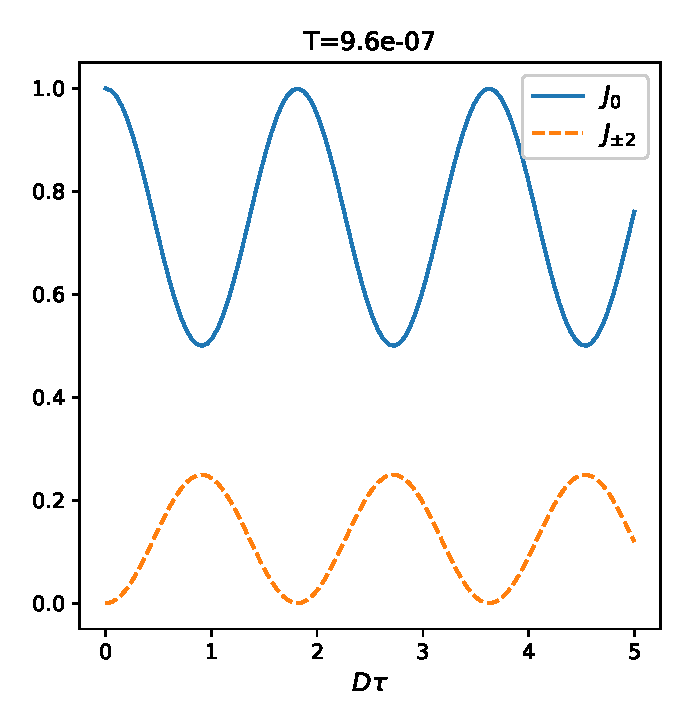
\includegraphics[width=0.5\linewidth]{coherences_n3_beta5.eps}
	\caption{
	  Интенсивности МК~когерентностей~ЯМР~$J_{n}$ ($n=0, 2$) в нанопоре с $N=3$.
      Здесь предполагается, что $\omega_{0} = 2\pi \cdot 500 \cdot 10^{6}$~s$^{-1}$ и $D = 2\pi \cdot 10^{4}$~s$^{-1}$.
	}
	\label{fig:1}
\end{figure}

В этом разделе будет получено точное решение МК~динамики~ЯМР~трехспиновой системы в дипольном упорядоченном состоянии в нанопоре.
Решение будет получена в общем виде, без использования высокотемпературного приближения~\cite{Goldman1970}.
Данная задача аналогична задаче, рассмотренной в разделе~\ref{sec:nanopora-thermodynamic-equilibrium}
для начального термодинамического равновесия в сильном внешнем магнитном поле.

Гамильтониан $H_{MQ}$ уравнения~(\ref{eq:hmq}) состоит из двух блоков для двух возможных значений углового момента спина $(I^2 = S(S+1), \quad S=3/2,1/2)$.
Эти блоки и соответствующие им собственные значения и собственные состояния приведены
в разделе~\ref{sec:sec:nanopora-thermodynamic-equilibrium-exact_sol}.
Матрица плотности системы также состоит из двух блоков $\rho^{3/2}(\tau)$, $\rho^{1/2}(\tau)$, и
%
\begin{equation}
  \label{eq:15}
  \rho^{3/2}(0) = \dfrac 1 Z
  \begin{pmatrix}
    e^{\frac{3b}{2}} & 0 & 0 & 0
    \\
    0 & e^{\frac{-3b}{2}} & 0 & 0
    \\
    0 & 0 & e^{\frac{-3b}{2}} & 0
    \\
    0 & 0 & 0 & e^{\frac{3b}{2}}
  \end{pmatrix},
  \quad
  \rho^{1/2}(0) = \dfrac 1 Z
  \begin{pmatrix}
    	1 & 0
    \\
    0 & 1
  \end{pmatrix}
\end{equation}
%
где $b = \dfrac{\hslash D}{k\mathrm{T}}$ и $T$ --- температура.
Простыми вычислениями можно получить матрицы плотности $\rho^{3/2}(\tau)$ и $\rho^{1/2}(\tau)$,
которые позволяют получить выражение для интенсивности МК~когерентностей~ЯМР.

В рассматриваемых системах появляются только МК~когерентности~ЯМР нулевого и плюс/минус второго порядков.
Интенсивности этих когерентностей равны
%
\begin{equation}
  \begin{split}
    \label{eq:16}
    J_0(\tau) & = 1
    - \dfrac 1 2 \tanh^2\left( \dfrac{3b}{2} \right)
      \sin^2 \left( \sqrt{3} Dt \right),
    \\
    J_{\pm2}(\tau) & = \dfrac{1}{4}
      \tanh^2 \left( \dfrac{3b}{2} \right)
      \sin^2 \left( \sqrt{3} Dt \right)
  \end{split}
\end{equation}
%
Сумма интенсивностей МК когерентностей согласно~(\ref{eq:16}) равна единице в соответствии с уравнением~(\ref{eq:14}).
Зависимости рассчитанных интенсивностей $J_{n}(\tau)$ $(n=0,2)$ от времени эволюции показаны на рисунке~(\ref{fig:1}).

% \subsection{Численный анализ многоспиновой запутанности при различных температурах и различном числе спинов в системе}
\subsection{Температурная зависимость многочастичной запутанности}
\label{sec:5}

В этом разделе приведены результаты полуаналитической симуляции МК эксперимента ЯМР
для модели спин-несущих молекул (атомов) в нанопоре в дипольном упорядоченном состоянии.
Будет рассмотрена зависимость нижней границы квантовой информации Фишера от времени и температуры.
А также получены оценки количества запутанных частиц в системе.
В расчетах предполагается, что $\omega_{0} = 2\pi \cdot 500 \cdot 10^{6}$~s$^{-1}$ и $D = 2\pi \cdot 10^{4}$~s$^{-1}$.

\begin{figure}[H]
 	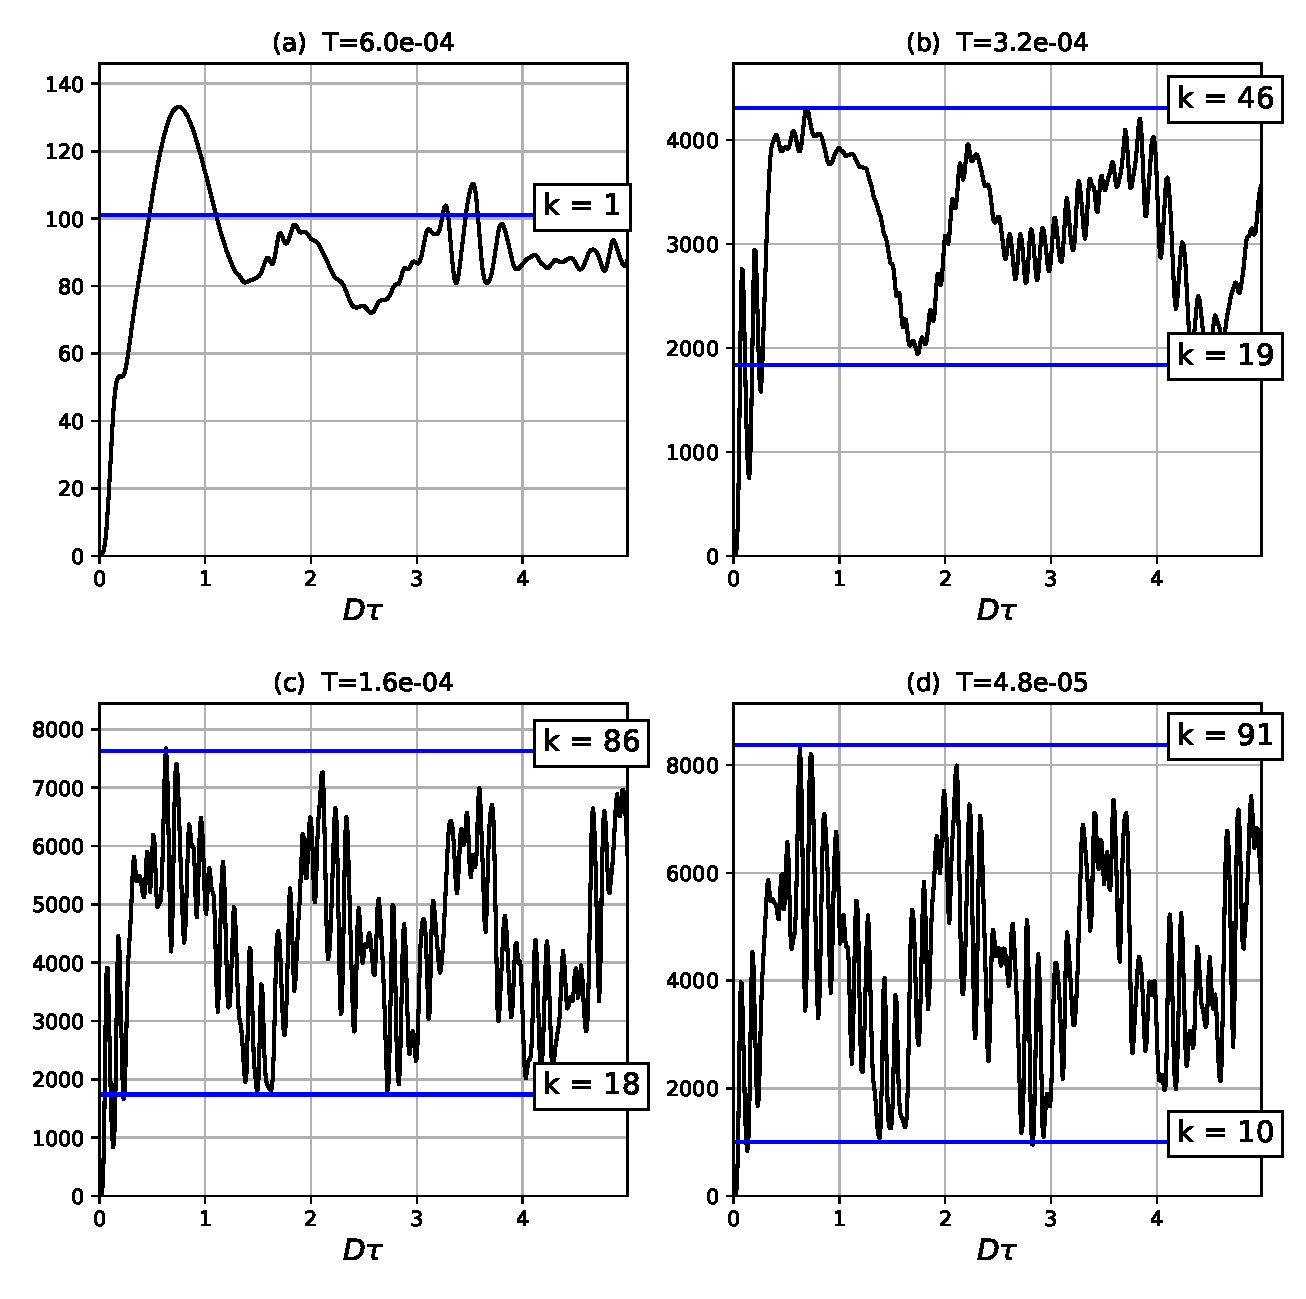
\includegraphics[width=0.95\linewidth]{fisher_low_bound_n101.eps}
	\caption{
	  Зависимость нижней границы  квантовой информации Фишера $F_\mathrm{Q} = 2 M_{2}$
	  от безразмерного времени $D\tau$ при $N=101$.
	  a) $T=6\cdot10^{-4}$~K, неравенство~(\ref{eq:20}) определяет область парной запутанности  (k+1=2), эта область выше горизонтальной линии;
	  b) $T=3.2\cdot10^{-4}$~K, область многоспиновой запутанности представляет собой полосу, ограниченную горизонтальными линиями с~$k=19$~и~$k=46$;
	  c) $T = 1.6\cdot10^{_4}$~K, горизонтальные линии ($k=18$ и $k=86$) ограничивают полосу с многоспиновой запутанностью;
	  d) при $T=4.8\cdot10^{-5}$~K возникают запутанные кластеры с $11-92$ спинами.
	}
	\label{fig:2}
\end{figure}


Рассматриваемая модель спин-несущих молекул (атомов) в нанопоре в дипольном упорядоченном состоянии
расширяет возможности исследования многоспиновой запутанности по сравнению с родственной моделью~(см. раздел~\ref{sec:nanopora-thermodynamic-equilibrium}),
в которой система изначально находилась в термодинамическом равновесии в сильном внешнем магнитном поле.
Модель из раздела~\ref{sec:nanopora-thermodynamic-equilibrium}) неприменима для исследования эволюции системы во времени,
потому что распределение МК~когерентностей~ЯМР~быстро становится стационарным~\cite{Doronin2009}.
Также многоспиновая запутанность изменяется с температурой в очень узком температурном интервале.
Например, все спины запутаны в системе, состоящей из 201 спина уже при температуре $T=6.856\cdot10^{-3}$~K~\cite{Doronin2019}.

Зависимость нижней границы квантовой информации Фишера от времени в системе, состоящей из 101 спина, представлена на Рис.~(\ref{fig:2}) при различных температурах.
Из Рис.~(\ref{fig:2}a) видно, что при температуре $T=6\cdot10^{-4}$~K существует только парная запутанность.
При температуре $T=3.2\cdot10^{-4}$ на Рис.~(\ref{fig:2}b) появляется полоса, в которой неравенство~(\ref{eq:entanglement-criteria}) может быть выполнено, когда $19 \leq k \leq 46$.
Таким образом, существует многоспиновая запутанность в спиновых кластерах, состоящих из 20-47 спинов, при температуре $3.2\cdot10^{-4}$~K.
Когда температура понижается, ширина полосы, в которой существует многоспиновая запутанность, увеличивается.
При температуре $T=1.6\cdot10^{-4}$~K (Рис.~(\ref{fig:2}c)) появляются кластеры из 19-87 запутанных спинов, а при температуре $T=4.8\cdot10^{-5}$~K (Рис.~(\ref{fig:2}d)), наблюдаются 11-92 запутанных спина.

\begin{figure}
 	\includegraphics[width=0.95\linewidth]{entangled_spins_by_n.eps}
	\caption{
	  Зависимость максимального количества запутанных спинов,
	  усредненного по времени эволюции $(0 \leq D\tau \leq 3)$,
	  от температуры при  a) $N=51$; b) $N=75$; c) $N=101$.
	}
	\label{fig:3}
\end{figure}

Зависимость максимального числа запутанных спинов за время эволюции $({0}\leq \mathrm{D}\tau\leq{3})$ от температуры при разных числах спинов в нанопоре представлена на Рис.~(\ref{fig:3}).
Максимальное количество запутанных спинов уменьшается при повышении температуры.
Максимальное количество запутанных спинов увеличивается, когда увеличивается число спинов в нанопоре, потому что система в нанопоре становится плотнее.

\section{Выводы}
\label{sec:conslusions}
% We investigated many-particle entanglement in MQ NMR spectroscopy using a nanocavity filled with spin-carrying atoms (molecules).
% We developed a theory of MQ NMR in a nanocavity at low temperatures.
% The theory is based on the idea that  molecular diffusion is substantially faster than the time of the spin flip-flop processes.
% As a result, the problem is reduced to a system of equivalent spins [23, 25], which can be analyzed in the basis of the common eigenstates of the total spin angular momentum and its projection on the external magnetic field.
% Since there is a connection between the second moment (dispersion) of the distribution of the MQ NMR intensities and many-spin entanglement [17], we extracted information about many-spin entanglement from the MQ NMR spectrum. The temperature dependence of many-spin entanglement was also investigated.
% \par
% The main lesson consists in significant growth of many-particle entanglement at low temperatures.
% All or almost all spins are entangled at the dimensionless temperature $\frac{1}{b}$ of the order of 1.
% This suggests that $k$-entangled states with large $k$ emerge in a typical MQ NMR system at low temperatures.
% This is particularly interesting given the absence of entanglement in the initial state. We expect such behavior to be typical for MQ NMR.
% \par
% We can conclude that MQ NMR spectroscopy is an effective method for the investigation of many-spin entanglement and the spreading of MQ correlations inside many-spin systems. It can be used for experimental investigations of quantum information processing in solids (note a related study of decoherence in liquids \cite{HOU2017863}).
% \par

В этой главе была исследована многочастичная запутанность в МК спектроскопии ЯМР в нанопоре, заполненной сотнями спин-несущими частицами.
Для этого была разработана МК теория ЯМР в нанопоре при низких температурах.
Было рассмотрено два начальных состояния системы:
термодинамически равновесное
и дипольное упорядоченное.
В обоих случах впервые удалось исследовать температурную зависимость многочастичной запутанности.
Все или почти все спины запутаны при безразмерной температуре $\frac{1}{b}$ порядка 1.
Это говорит о том, что $k$-запутанные состояния с большим $k$ возникают в типичной системе МК ЯМР при низких температурах.
Это особенно интересно, учитывая отсутствие запутанности в начальном состоянии.
Можно заключить, что такое поведение типично для МК ЯМР.
Так же была исследована зависимость многоспиновой запутанности
от количества спинов в нанопоре.
Показано, что с ростом количества спинов в нанопоре,
скорость возникновения запутанных кластеров при понижении температуры увеличивается.

Результаты этого раздела наглядно демонстрируют
универсальность разработанного в этой диссертации метода исследования многочастичной запутанности.

% \chapter{Многоспиновая запутанность в зигзагообразной цепочке}
\chapter{Многоспиновая запутанность в квазиодномерных цепочках}
\label{chapter:manayparticle-entantlement-in-zigzag-chain}
% AMR-2020


% \begin{figure}
%   \includegraphics[width=0.5\textwidth]{model-zigzag-chain-schema.png}
%   \caption{Схема зигзагообзаной цепочки}
% \end{figure}
%
%     Константы взаимодействия
%         $$D_1=\dfrac{\gamma^2\hbar }{r^3}, $$
%         $$D_2 = D_1\dfrac{ 3\cos^2 \varphi -1 }{2} $$
%         $$D_3 = D_1 \dfrac{ 3\sin^2 \frac{\varphi}{2} -1}{16 \sin^3, \frac{\varphi}{2}}$$
%         где $\gamma$ - гиромагнитное отношение,
%         $\varphi$ - угол между соседними связями,
%         $r$ - расстояние между соседними спинами в цепочке.
%
%     Базовый случай это когда одна линия связи направлена вдоль поля. тогда констаты будет самой большой в доль поля.
%     Изменяя угол к полю мы можем получить как альтернированную цепочку так и однородную.
%     В приближении ближайших и следующих соседей, задача решается аналитически, но она
%     не дает полной картины. Поэтому мы решали данную систему численно.
%
%     \begin{figure}
%       \includegraphics[width=0.85\textwidth]{model-zigzag-chain-hambergite-structure.png}
%       \caption{Hанопора со спин-несущих молекулами во внешнем сильном магнитном поле $\vec B$}
%     \end{figure}
%
%     Гамбергит $Be_2BO_3(OH)$
%         \begin{itemize}
%             \item Дипольное взаимодействия между ближайшими спинами протонов в цепи в 17 раз сильнее, чем со спинами окружающих цепей (в худшем случае).
%             \item Взаимодействия с остальными окружающими спинами по меньшей мере в 30 раз слабее.
%             \item Вклад дипольной связи между спинами в одной и той же цепи доминирует над остальными взаимодействиями.
%         \end{itemize}
%
%     В одномерных цепочках возникают когерентности только $\pm 2$ порядка
%     и следовательно дисперсия распределения будет небольшой
%     и мы не увидим запутанных кластеров.
%     Однако в альтернированная цепочке гамбергита возникают когерентности $\pm 4$ порядка
%     и следовательно можно использовать эту модель для исследования многочастичной запутанности.
%     The distance to these two protons is 4.49~\r{A}
%     The distance between a given chain and surrounding proton chains is at least 2.1 times larger than the distance between neighbors in the chain.
%

В предыдущей главе~\ref{chapter:manyparticle-entanglement-in-nanopore}
была подробно исследована многочастичная запутанность,
возникающая в МК эксперименте ЯМР в нанопоре.
Данная модель показала себя отличной площадкой
для исследования запутанности многих взаимодействующих частиц.
Тем не менее одномерные модели значительно лучше изучены как теоретически,
так и экспериментально~(см. раздел~\ref{sec:model-uniform-chain}).
В этой главе будет исследована многочастичная запутанность возникающая в таких системах.


\section{Однородная цепочка}
Однородная цепочка является наиболее простой разновидностью одномерной системы.
Создание запутанных кластеров в таких цепочках ограничено слабыми ДДВ удаленных спинов.
В МК эксперименте ЯМР в однородной цепочке возникают когерентности только нулевого и плюс/минус второго порядков.
Оценка снизу информации Фишера может быть получена с помощью Гауссова приближения для распределения интенсивностей МК когерентностей~\cite{Baum1985}.
В этом случае выражение для МК когерентностей имеет
%
\begin{equation}\label{eq:gaussaprox}
  J(\tau, T)=\dfrac{1}{\sqrt{\pi N_c(T)}} \exp\p{-\frac{n^2}{N_c(T)}},
\end{equation}
%
где $N_c(T)$ это число коррелированных спинов,
ответственных за создание профиля МК когерентности.
Поскольку удвоенный второй момент интенсивностей МК когерентностей $2M_2(\tau, T)$ является нижней границей квантовой информации Фишера $F_Q$
(см.~раздел~\ref{sec:quantum-fisher-information-mesuarement-at-high-temperature})
из уравнения~(\ref{eq:gaussaprox}) можно найти, что
%
\begin{equation}\label{eq:qfisheinf}
  F_Q \geq 2M_2(\tau, T) = N_c(T) \geq N,
\end{equation}
%
где $N$ --- число узлов в цепочке.
Для небольших значений $k$ верхнюю границу информации Фишера $k$-сепарабельного состояния
$F^k_Q = \sup{F_Q\p{\rho_{k-\mathrm{prod}}}}$~(см.~раздел.~\ref{sec:manyparticle-entanglement-criteria}) можно переписать в приближённой форме как
%
\begin{equation}\label{eq:inequalityforfq2}
  F^k_Q \leq k N.
\end{equation}
%
Неравенство~(\ref{eq:inequalityforfq2}) не нарушается ни для какого $k > 0$, когда $F_Q = N$,
а для случая $F_Q > N$ детектируется только парная запутанность.
Полученная оценка согласуется с представленными в литературе~\cite{Doronin2007, Feldman2012} результатами.

Из выражения~(\ref{eq:qfisheinf}) также следует,
что увеличение числа узлов цепочки не способствует детектированию запутанных кластеров большего размера, чем двухчастичный.
Тем не менее этого достаточно для передачи МК когерентностей вдоль цепочки~\cite{Bochkin2018qip} и создания запутанности между удаленными концами цепочки~\cite{Lazarev2019}.

% \subsection{Температурная зависимость запутанности удаленных узлов цепочки}
\subsection{Запутанность удаленных узлов цепочки}
\label{subsec:entanglement-of-remote-chain-nodes}
Однородная цепочка является удобной моделью линии связи для передачи квантовых состояний на короткие расстояния.
Типичная схема линии связи (см.~Рис.\ref{fig:model-uniform-chain-schema}) состоит из передатчика (sender $S$),
приемника (reciever $R$)
и линии передачи (transmition line $TL$).
Также ряд протоколов передачи задействуют расширенный приемник (extended reciever $ER$),
на котором применяется специально сконструированное универсальное унитарное преобразование для наилучшего восстановления передаваемой информации~\cite{Feldman2021}.

\begin{figure}[H]
  \centering
  \includegraphics[width=0.9\textwidth]{model-uniform-chain-schema.png}
  \caption{
    Схематичное изображение линии передачи квантовых состояний.
    S --- передатчик,
    TL --- линия передачи,
    ER --- расширенный приемник,
    R --- приемник.
  }
  \label{fig:model-uniform-chain-schema}
\end{figure}

В оригинальной работе Бозе~\cite{Bose2003} был рассмотрен случай передачи однокубитного состояния под действием Гейзенберговского Гамильтониана.
В рамках МК спектроскопии ЯМР более естественно рассматривать передачу под действием $XX$-Гамильтониана,
который для однородной цепочки совпадает с МК Гамильтонианом $H_\mathrm{MQ}$~(\ref{eq:hmq}) с точностью до поворота~(см.~раздел~\ref{sec:model-uniform-chain}).
В приближении ближайших соседей во вращающейся системе координат с Ларморовской частотой $\omega_0$ выражение $XX$-Гамильтониана имеет вид:
%
\begin{equation}\label{eq:hxx}
  H_\mathrm{XX} = D\sum_{j=1}^{N-1}\p{I_{j,x}I_{j+1,x} + I_{j,y}I_{j+1,y}},
\end{equation}
где $D$ --- константна ДДВ между соседними узлами,
а N --- число узлов в цепочке.
В базисе бесспиновых фермионных операторов $\gamma_j$ and $\gamma_j ^+$
гамильтониан~(\ref{eq:hxx}) имеет диагональный вид
\begin{equation}\label{Diagonal_Hamiltonian}
  H_\mathrm{XX}=\sum\limits _{k}\varepsilon _{k}\gamma ^{+}_{k}\gamma _{k}.
\end{equation}
Переход к новому базису определяется преобразованием Йордана-Вигнера~\cite{Jordan1928, Feldman1998}:
\begin{equation}\label{eq:jw_operators}
  \gamma _{k}=\sum\limits ^{N}_{j=1}g_{kj} c_{j},
  \quad
  \gamma^+ _{k}=\sum\limits ^{N}_{j=1}g_{kj} c_{j}^+,
\end{equation}
где операторы рождения/уничтожения
\begin{equation}\label{eq:creation_annihilation_operators}
  c_{j}=(-2)^{j-1}I_{1,z}I_{2,z}I_{3,z}...I_{j-1,z}I^-_j,
  \quad
  c_{j}^+=(-2)^{j-1}I_{1,z}I_{2,z}I_{3,z}...I_{j-1,z}I^+_j,
\end{equation}
и
\begin{equation}\label{eq:gammakj}
  \varepsilon_{k} = D \cos(k),
  \quad
  g_{kj} =\sqrt {\frac {2}{N+1}}\sin \left( kj\right),
  \quad
  k=\frac {\pi n}{N+1}\quad n=1\ldots N .
\end{equation}

В общем случае в начальный момент времени однокубитный передатчик --- это произвольное чистое состояние
%
\begin{equation}\label{eq:random-pure-state}
  \ket{\psi_\mathrm{init}} = a\ket{0} + b\ket{1},
  \quad
  |a|^2 + |b|^2 = 1,
\end{equation}
%
а линия передачи и приемник находятся в термодинамическом равновесном состоянии
%
\begin{equation}
    \rho^\mathrm{TL, R}_\mathrm{init} = \otimes_{i=2}^N e^{\beta I_{i, z}}.
\end{equation}

Эволюционная матрица плотности может быть найдена из стационарного уравнения Лиювилля
\begin{equation}\label{eq:eval-rho-liuville}
  \rho(t) = e^{-iH_\mathrm{XX}t}
    \ket{\psi_\mathrm{init}} \bra{\psi_\mathrm{init}}
    \otimes
    \rho^\mathrm{TL, R}_\mathrm{init}
    e^{iH_\mathrm{XX}t}.
\end{equation}
После проведения редукции эволюционной матрицы плотности $\rho(t)$~(\ref{eq:eval-rho-liuville}) по линии передачи,
матрица плотности и приемника определяется выражением
%
\small
\begin{equation}\label{eq:eval-rho-sr}
\rho^\mathrm{S,R}(t) =
\begin{pmatrix}
  \begin{array}{r}
    L(|f|^2+|g|^2) \\
    + \frac{e^{2\beta}}{(e^{\beta}+1)^2}
  \end{array}
  &
  \begin{array}{r}
    -\p{-\tanh\frac{\beta}{2}}^{N-2} \\
    \times \frac{ab^*f^* e^{\frac{\beta}{2}}}{2\cosh\frac{\beta}{2}}
  \end{array}
  &
  \frac{ab^* e^{\beta /2}}{2\cosh\frac{\beta}{2}}g^*
  &
  0\\
  &
  &
  &\\
  \begin{array}{r}
    -\p{-\tanh\frac{\beta}{2}}^{N-2} \\
    \times\frac{a^*bf e^{\frac{\beta}{2}}}{2\cosh\frac{\beta}{2}}
  \end{array}
  &
  \begin{array}{r}
    L(e^{-\beta}|g|^2-|f|^2) \\
    +\frac{1}{2\cosh{\beta}+2}
  \end{array}
  &
  \begin{array}{r}
    {2\p{-\tanh\frac{\beta}{2}}^{n-2}}\\
    \times Lfg^*\cosh\frac{\beta}{2}
  \end{array}
  &
  \frac{ab^* e^{-\beta/2}}{2\cosh\frac{\beta}{2}}g^* \\
  &
  &
  &\\
  \frac{a^*b e^{\beta /2}}{2\cosh\frac{\beta}{2}}g
  &
  \begin{array}{r}
   2\p{-\tanh\frac{\beta}{2}}^{n-2}\\ \times{Lf^*g\cosh\frac{\beta}{2}}
  \end{array}
  &
  \begin{array}{r}
    L(e^{-\beta}|f|^2 -|g|^2) \\
    +\frac{1}{2\cosh{\beta}+2}
  \end{array}
  &
  \begin{array}{r}
    \p{-\tanh\frac{\beta}{2}}^{N-2} \\
    \times \frac{ab^*f^* e^{-\frac{\beta}{2}}}{2\cosh\frac{\beta}{2}}
  \end{array}
  &
  &
  &\\
  0
  &
  \frac{a^*b e^{-\beta /2}}{2\cosh\frac{\beta}{2}}g
  &
  \begin{array}{r}
    \p{-\tanh\frac{\beta}{2}} ^{N-2} \\
    \times \frac{a^*bf e^{-\frac{\beta}{2}}}{2\cosh\frac{\beta}{2}}
  \end{array}
  &
  \begin{array}{r}
    -L e^{-\beta}(|f|^2 +|g|^2)\\
    + \frac{1}{(e^{\beta}+1)^2}
  \end{array}
\end{pmatrix},
\end{equation}
\normalsize
где $f={f_N(t, N)}$, $g={f_N(t, 1)}$, $L=\frac{1-2|b|^2 e^{\frac{\beta}{2}}\cosh\frac{\beta}{2}}{\cosh\frac{\beta}{2}}$
и
%
\begin{equation}
  f_N(t, j) = \frac{2}{N+1}\sum_k e^{i\epsilon_k t}\sin k \sin jk.
\end{equation}

\begin{figure}[H]
  \begin{subfigure}{0.45\textwidth}
    \includegraphics[width=\textwidth]{concurence-temp-uniform-chain-N4.png}
    \caption{
      $\ket{\psi} = \dfrac{\ket{0} + \ket{1}}{\sqrt{2}}$
    }
    \label{fig:concurence-temp-uniform-chain-N4}
  \end{subfigure}
  \hfill
  \begin{subfigure}{0.45\textwidth}
    \includegraphics[width=\textwidth]{concurence-polarization-uniform-chain-N4.png}
    \caption{
      $\beta = 5$
    }
    \label{fig:concurence-polarization-uniform-chain-N4}
  \end{subfigure}
  \caption{
    Зависимость согласованности $C$ от безразмерного времени $\tau = Dt$,
    обратной температуры $\beta$
    (cм. Рис.~\ref{fig:concurence-temp-uniform-chain-N4})
    и величины поляризации $|b|$
    (cм. Рис.~\ref{fig:concurence-polarization-uniform-chain-N4})
    при передаче квантового состояния по цепочке из $N=4$ спинов.
  }
  \label{fig:councurence-uniform-chain-N4}
\end{figure}

В качестве критерия запутанности для двухкубитного смешанного состояния удобнее всего использовать критерий Вуттерса~(см. раздел. ~\ref{sec:entanglement-criteria}) на основе величины согласованности $C$.
Температурная зависимость согласованности $C$ при передаче в чистого состояния $\ket{\psi} = \frac{\ket{0} + \ket{1}}{\sqrt{2}}$ ($a=b=\frac{1}{\sqrt{2}}$) представлена на Рис.~\ref{fig:concurence-temp-uniform-chain-N4}.
При обратной температуре $\beta > 1$ приемник и передатчик запутываются.
На Рис.~\ref{fig:concurence-polarization-uniform-chain-N4} представлена зависимость согласованности $C$ от различных значений начальной поляризации передатчика при температуре $\beta = 5$.
Приемник и передатчик запутываются при любой начальной поляризации.

\begin{figure}[H]
    \centering
    \includegraphics[width=0.8\textwidth]{fidelity-n-beta.png}
    \caption{
      Зависимость фиделити переданного состояния
      $\rho^\mathrm{S}_\mathrm{init}$
      и полученного
      $\rho^\mathrm{R}\p{\bar\tau_N}$
      от количества узлов в цепи.
      Разные линии соответствуют разным значениям обратной температуры $\beta$.
     }
    \label{fig:fidelity-n-beta}
\end{figure}

Идеальная передача произвольного квантового состояния в спиновых цепочках достижима только в очень специфических случаях~\cite{Christandl2004, Karbach2005} и может быть легко разрушена небольшими возмущениями гамильтониана взаимодействия.
В общем случае передача осуществляться не идеально,
но с высокой вероятностью.
Качество передачи можно оценить с помощью фиделити~\cite{Jozsa1994}
%
\begin{equation}\label{generalFidelity}
  F\p{\rho^\mathrm{S}_\mathrm{init}, \rho^\mathrm{R}\p{t}}
  = \tr{\rho^\mathrm{S}_\mathrm{init}, \rho^\mathrm{R}(t)}.
\end{equation}
%
С учетом $\rho^\mathrm{R}\p{t} = \tr{\rho^\mathrm{S,R}(t)}_\mathrm{S}$,
аналитическое выражение для фиделити имеет вид
%
\begin{multline}\label{exactfidelity}
  F\p{\rho^\mathrm{S}_\mathrm{init}, \rho^\mathrm{R}\p{t}}
  = (1-2|b|^2)\p{
    \frac{e^{\beta/2}}{\cosh \beta/2}
    + \p{\frac{e^{-\beta/2}}{\cosh \beta/2} -|b|^2 }
      \left|f_N(t, N)\right|^2
  } \\
  + |b|^2
  + 2 |b|^2 \p{1-|b|^2} \Re\left\{f_N(t, N)\right\}
  \p{-\tanh \p{\frac{\beta}{2}}}^{N-1}.
\end{multline}
%
Время $\bar\tau_{N}$, при котором фиделити достигает первого пика, называется временем передачи~\cite{Feldman2016}.
Оно совпадает с временем первого пика функции $\left|f_N(t, N)\right|^2$.
Фиделити~\cite{Jozsa1994} переданного и полученного квантового состояния в момент времени $\bar\tau_{N}$ уменьшается с увеличением длинны цепочки (см. Рис.\ref{fig:fidelity-n-beta}).


\subsection{Идеальная передача запутанных состояний}
% \subsection{Идеальная передача МК когерентности нулевого порядка}

Гамильтониан $H_\mathrm{XX}$ коммутирует с $z$-проекцией $I_z$ полного спинового момента
и сохраняет число возбуждений в процессе эволюции.
В этом случае когерентности разных порядков не перемешиваются~\cite{Feldman2017} и могут быть рассмотрены отдельно~\cite{Bochkin2018qip}.
В частности было показано~\cite{Feldman2021},
что специальная форма когерентности нулевого порядка может передаваться без потерь
по цепочке из $N$ узлов находящейся в основном состоянии:
%
\begin{equation}
  \rho^\mathrm{TL}_\mathrm{init} = \otimes^{N_\mathrm{TL}}_{i=1}\ket{0},
  \quad
  \rho^\mathrm{R}_\mathrm{init} = \otimes^{N_\mathrm{R}}_{i=1}\ket{0},
\end{equation}
%
где $N_\mathrm{R}$ --- количество кубитов в приёмнике,
а $N_\mathrm{TL}  = N - 2 N_\mathrm{R}$.
В случае, когда количество кубитов в передатчике $N_\mathrm{S} = N_\mathrm{R} = 3$,
специальная матрица плотности передатчика,
которая может быть передана без потерь,
в базисе с одним возбуждением
$\left \{\ket{000}, \ket{001}, \ket{010}, \ket{100} \right\}$
может быть записана в виде
%
\begin{equation}
  \rho^\mathrm{S}_\mathrm{init} =
  \begin{pmatrix}
    u &    0     &    0    & 0 \\
    0 &   x_1    & \omega  & 0 \\
    0 & \omega^* &   x_2   & 0 \\
    0 &    0     &    0    & v
  \end{pmatrix}.
\end{equation}
%
После редукции $\rho^\mathrm{S}_\mathrm{init}$ по первому спину
матрица плотности оставшихся двух в полном базисе имеет вид
\begin{equation}\label{eq:rho-s-reduced}
  \tr{\rho^\mathrm{S}_\mathrm{init}}_{1} =
  \begin{pmatrix}
    u + v &    0     &    0    & 0 \\
    0     &   x_1    & \omega  & 0 \\
    0     & \omega^* &   x_2   & 0 \\
    0     &    0     &    0    & 0
  \end{pmatrix}.
\end{equation}
Для матрицы вида~(\ref{eq:rho-s-reduced}) согласованность $C$
определяется~(cм.~раздел~\ref{sec:entanglement-criteria}) только величиной недиагональных элементов:
%
\begin{equation}
  C = 2 |w|.
\end{equation}


\begin{figure}[H]
    \centering
    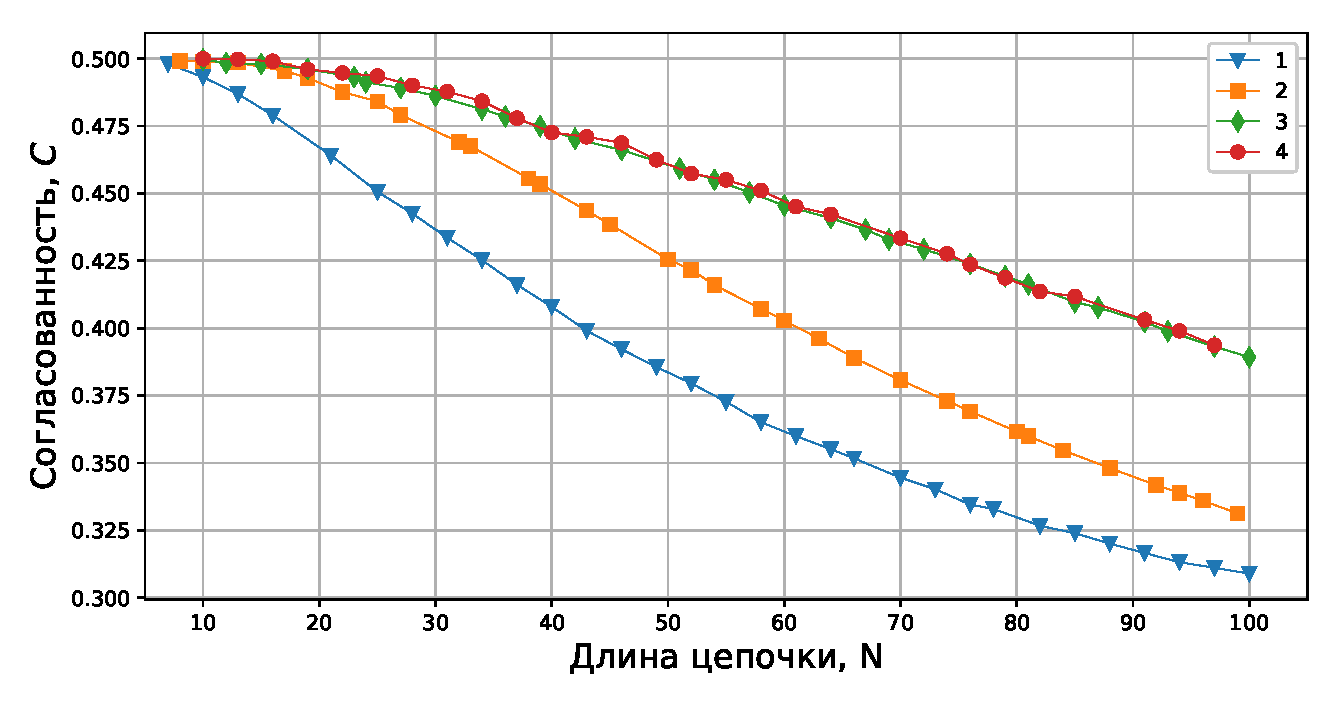
\includegraphics[width=0.9\textwidth]{concurence-n-s3.eps}
    \caption{
      Максимальное значение согласованности второго и третьего спинов передатчика, состояние которого может быть передано без потерь,
      от количества узлов в цепи.
      Разные линии отвечают разным размерам расширенного приемника.
    }
    \label{fig:concurence-n-s3}
\end{figure}


Так как элементы матрицы плотности, вносящие вклад в каждую когерентность, перемешиваются в процессе эволюции,
на расширенном приемнике ER применятся специальное унитарное преобразование $U^\mathrm{ER}(\phi)$ для их распутывания~\cite{Feldman2017}.
По аналогии с работой~\cite{Bochkin2022} можно подобрать такое унитарное преобразование на расширенном приемнике,
которое позволяет передавать состояния с максимальным значением согласованности второго и третьего спинов передатчика.
На Рис.~\ref{fig:concurence-n-s3} приведены максимально возможные значения согласованности от длины цепочки,
полученные путем максимизации модуля недиагонального элемента $\omega$ матрицы плотности $\rho^\mathrm{S}_\mathrm{init}$ по параметрам унитарного преобразования $U^\mathrm{ER}(\phi)$.
Вычисления выполнены с помощью метода дифференциальной эволюции~\cite{Storn1997,Wormington1999,Lampinen2002} из библиотеки SciPy~\cite{SciPy} версии 1.4.1.


\section{Зигзагообразная цепочка}
В зигзагообразных цепочках в кристалле гамбергита в МК эксперименте ЯМР,
в отличие от однородных цепочек,
возникают когерентности плюс/минус четвертого порядка (см. раздел~\ref{sec:model-zigzag-chain}).
Данное обстоятельство является важным для исследования многоспиновой запутанности,
поскольку при этом используется второй момент распределения МК когерентностей ЯМР.

\begin{figure}[H]
    \centering
    \includegraphics[width=0.3\textwidth]{model-zigzag-chain-schema}
    \caption{
      Зигзагообразная цепочка ядерных спинов.
      Нечетные звенья параллельны внешнему магнитному полю $\vec{\mathcal H}_0$,
      а $\varphi$ - угол между соседними звеньями.
      Константы связи $D_1$ и $D_2$ определяются уравнением~(\ref{eq:dipolaconstantsnearest}), а $D_3=D_{n, n+2},\, (n=1,2,...)$
      уравнением~(\ref{eq:dipolaconstantsnextnearest}).
    }
    \label{fig:model-zigzag-chain-schema}
\end{figure}

На Рис.~\ref{fig:model-zigzag-chain-schema} схематично представлена
зигзагообразная цепочка ядерных спинов в сильном внешнем магнитным полем $\vec{\mathcal H}_0$.
Нечетные звенья цепочки параллельны внешнему магнитному полю $\vec{\mathcal H}_0$,
а $\varphi$ - угол между соседними звеньями.
Гамильтониан $H_\mathrm{MQ}$,
описывающий МК динамику ЯМР~(см. раздел~\ref{sec:mq-nrm-experiment}),
задается выражением~\cite{Doronin2000}
%
\begin{equation}\label{hmqnextnearest}
 H_\mathrm{MQ} = \sum_{i=1}^{N-1} D_{i, i+1}(I_i^{+}I_{i+1}^{+}+ I_i^{-}I_{i+1}^{-} )
   + \sum_{i=1}^{N-2} D_{i, i+2}(I_i^{+}I_{i+2}^{+}+ I_i^{-}I_{i+2}^{-} ) ,
\end{equation}
%
где $I_i^+$, $I_i^-$ --- это повышающей и понижающий операторы спинового углового момента спина с номером $i$,
и $N$ --- это количество ядерных спинов в цепочке.

Константы диполь-дипольного взаимодействия (ДДВ)
в зигзагообразной цепочке определяются выражениями~\cite{Abragam1982}
%
\begin{equation}\label{eq:dipolaconstantsnearest}
  D_{2n-1, 2n} = D_1 =\dfrac{\gamma^2\hbar }{r^3},
  \quad
  D_{2n, 2n+1} = D_2=\dfrac{\gamma^2\hbar }{2r^3}\p{3\cos^2 \varphi -1},
  \quad
  n=1,2\dots,
\end{equation}
где $\gamma$ --- это гиромагнитное отношение,
и $r$ --- это расстояние между ближайшими спинами в цепочке.
Также в гамильтониане учитываются взаимодействия со следующими соседями,
константа диполь-дипольного взаимодействия которых определяется как~\cite{Abragam1982}
%
\begin{equation}\label{eq:dipolaconstantsnextnearest}
  D_{n, n+2}=\dfrac{\gamma^2\hbar }{16r^3 \sin^3 \frac{\varphi}{2}}\p{3\sin^2 \frac{\varphi}{2} -1}.
\end{equation}
%
В частности, уравнения~(\ref{eq:dipolaconstantsnearest}),~(\ref{eq:dipolaconstantsnextnearest}) означают,
что для прямой спиновой цепочки, когда  $(\varphi=\pi)$,
константа дипольной связи для ближайших соседей в восемь раз больше,
чем константа дипольной связи между следующими ближайшими соседями.
Тем не менее при $\varphi=\frac{2\pi}{3}$ отношение констант связи
\begin{equation}
  \left|\dfrac{D_{2n, 2n+1}}{D_{2n-1, 2n+1}}\right| = \dfrac{3\sqrt{3}}{5},
\end{equation}
и, следовательно,
диполь-дипольные взаимодействия следующих ближайших соседей
существенны для МК динамики ЯМР при определённых ориентациях зигзагообразной спиновой цепочки
по отношению к направлению внешнего сильного магнитного поля.


\subsection{Температурная зависимость многочастичной запутанности}
Для исследования температурной зависимости многочастичной запутанности
в зигзагообразных цепочках
в этом разделе будет рассмотрена МК динамика ЯМР
на подготовительном периоде МК эксперимента ЯМР~(см. раздел~\ref{sec:mq-nrm-experiment})
с начальным термодинамически равновесным состоянием $\rho_\mathrm{eq}$.
Матрица плотности системы в начальный момент времени имеет вид:
\begin{equation}
  \rho(0, \beta)
  = \rho_\mathrm{eq}
  = \dfrac{e^{\frac{\hbar\omega_{0}}{kT} I_z}}{Z},
  = \dfrac{e^{\beta I_z}}{Z},
\end{equation}
где $Z = \tr{e^{\beta I_z}}$ --- статистическая сумма,
$\hslash$ и $k$ --- константы Планка и Больцмана,
$\omega_{0}$ --- частота Лармора,
$I_\mathrm{z}$ ---  оператор проекции полного углового спинового момента  на ось~$z$,
который направлен вдоль сильного внешнего магнитного поля.

Интенсивности приведенных МК когерентностей ЯМР определяются уравнением~\ref{eq:reduced-mq-coherences}~(см. раздел~\ref{sec:reduced-mq-coherences}).
Для $b=0.5$,
что соответствует температуре $T=4.8 \times 10^{-2}\,\mbox{K}$
при Ларморовской частоте $\omega_0=2\pi\times 500\times 10^6 \,\mbox{s}^{-1}$,
было обнаружено,
что неравенство~(\ref{eq:entanglement-criteria}) может быть выполнено только при $k=1$ для спиновых цепочек с $N=6$ и $N=8$.
Это означает, что в высокотемпературном случае~\cite{Doronin2019}
детектируется парная запутанность,
что согласуется с работой~\cite{Feldman2012}.

\begin{figure}[H]
  \begin{subfigure}[t]{0.49\textwidth}
    \includegraphics[width=\textwidth]{m2-by-time-in-zigzag-chain-with-n6-beta10}
    \caption{
      Зависимость нижней границы квантовой информации
      Фишера~$F_Q=2M_2(\tau, T)$
      от безразмерного времени~$D_1\tau$
      для зигзагообразной цепочки из 6 спинов
      при температуре $2.4\times 10^{-3}\,\mbox{K}$ $(b=10)$.
      В области выше горизонтальной линии $k=1$
      гарантировано существует как минимум парная запутанность.
      В области выше горизонтальной линии $k=5$
      гарантировано существует шестиспиновая запутанность.
    }
    \label{fig:fig3}
  \end{subfigure}
  \hfill
  \begin{subfigure}[t]{0.49\textwidth}
    \includegraphics[width=\textwidth]{nent-by-n-b10}
    \caption{
      Зависимость оценки максимального количества запутанных спинов $N_{ent}$ от длины цепочки при температуре $2.4\times 10^{-3}\,\mbox{K}$.
    }
    \label{fig:fig4}
  \end{subfigure}
  \caption{}
\end{figure}

Зависимости многоспиновой запутанности от длины цепочки $N$ и температуры исследованы для спиновых цепочек с $4\leqslant N \leqslant 12$.
Временная эволюция нижней границы квантовой информации Фишера,
соответствующая  удвоенному второму моменту распределения интенсивностей МК когерентностей для шестиспиновой цепочки представлена на Рис.~\ref{fig:fig3} при температуре $2.4\times 10^{-3}\,\mbox{K}$ $(b=10)$.
На Рис.~\ref{fig:fig3} видна полоса,
в которой неравенство~(\ref{eq:entanglement-criteria}) может быть удовлетворено при $1\leqslant k \leqslant 5$.
Таким образом, существует многоспиновая запутанность в спиновых кластерах, состоящих из 2-6 спинов при температуре $2.4\times 10^{-3}\,\mbox{K}$.
Зависимость оценки максимального количества запутанных спинов от длины цепи приведена на Рис.~\ref{fig:fig4} при температуре $2.4\times 10^{-3}\,\mbox{K}$.

\begin{figure}[H]
  \begin{subfigure}[t]{0.49\textwidth}
    
\includegraphics[width=\textwidth]{m2-by-time-in-zigzag-chain-with-n8-beta1}
    \caption{
      При температуре $2.4\times 10^{-2}\,\mbox{K}$
      в области ограниченной горизонтальными линиями $k=1$ и $k=2$
      присутствует как минимум парная запутанность.
    }
    \label{fig:fig5}
  \end{subfigure}
  \hfill
  \begin{subfigure}[t]{0.49\textwidth}
    \includegraphics[width=\textwidth]{m2-by-time-in-zigzag-chain-with-n8-beta10}
    \caption{
       При температуре $1.2\times 10^{-3}\,\mbox{K}$
       в области ограниченной горизонтальными линиями $k=2$ и $k=4$
       наблюдается как минимум трехчастичная запутанность.
    }
    \label{fig:fig6}
  \end{subfigure}
  \caption{
    Временная эволюция нижней границы информации Фишера~$F_Q=2M_2(\tau, T)$
    от безразмерного времени~$D_1\tau$
    в восьмиспиновой зигзагообразной цепочке.
  }
\end{figure}

Временная эволюция восьмиспиновой зигзагообразной цепочки представлена при $T=2.4\times 10^{-2}\,\mbox{K}$ (Рис.~\ref{fig:fig5}) и $T=1.2\times 10^{-2}\,\mbox{K}$ (Рис.~\ref{fig:fig6}).  Видно, что при температуре $T=2.4\times 10^{-2}\,\mbox{K}$ возникают многоспиновые запутанные кластеры, состоящие из двух или трех спинов, а при температуре $T=1.2\times 10^{-2}\,\mbox{K}$ возникают кластеры с $2\leqslant k \leqslant 5$.
Число запутанных спинов увеличивается с понижением температуры.

\begin{figure}[H]
  \centering
  
\includegraphics[width=0.6\textwidth]{nent-by-beta-n8-n6}
  \caption{
    Зависимость оценки максимального числа запутанных спинов от обратной температуры $b$
    для зигзагообразной цепочки,
    состоящей из шести и восьми спинов.
    }
    \label{fig:fig7}
\end{figure}

Зависимость числа запутанных спинов от температуры для зигзагообразных цепочек,
состоящих из шести или восьми спинов, приведена на Рис.~\ref{fig:fig7}.
% В этих цепочках почти все спины запутаны при низких температурах.
Так же как и в случае системы эквивалентных спинов,
при низких температурах почти все спины в цепочке запутанны.
% Результаты получены на небольшом интервале времени,
% поэтому эффектами декогеренции можно пренебречь.


% The creation of entangled clusters in the considered zigzag chains is limited by weak DDIs of remote spins.  Accordingly, that process requires a large time interval. Practically, the role of decoherence gets very important in that case.  We note also that the analysis of the inequality \eqref{inequalityforfq} shows that an increase in chain length does not result in an increase of the number of the entangled spins even at long times. Indeed, we can rewrite \eqref{inequalityforfq} in the approximate simple form
% \begin{equation}\label{inequalityforfq2}
% F_Q>k N.
% \end{equation}
% In order to estimate the Fisher information we use the Gaussian approximation for the distribution of the intensities of MQ coherences \cite{baum}
% \begin{equation}\label{gaussaprox}
% J(\tau, T)=\dsfrac{1}{\sqrt{\pi N_c(T)}} \exp\p{{-\frac{n^2}{N_c(T)}}},
% \end{equation}
% where $N_c(T)$ is the number of the correlated spins which are responsible for the creation of the MQ coherence profile. Since twice the second moment $2M_2(\tau, T)$ is a lower bound on the quantum Fisher information $F_Q$ \cite{toth, pezze} one can find from Eq. \eqref{gaussaprox} that
% \begin{equation}\label{qfisheinf}
% F_Q=N_c(T).
% \end{equation}
% Since $N\geqslant N_c(T)$, one can conclude that in the Gaussian model \cite{baum} only two-spin entanglement is possible.
%
% Numerical calculations for the zigzag spin chain yield similar results. We find that the Fisher information depends only weakly on the number of spins. It means (see Eq. \eqref{inequalityforfq2}) that the number of the entangled spins decreases when $N$ increases. We have found that in the zigzag six-spin system all six spins can be entangled. On the contrary, only three spins are entangled in the zigzag ten-spin system.
%
% Finally, the number of the entangled spins for the zigzag chain with $4\leqslant N\leqslant 12$ increases with decreasing temperature.


\section{Выводы}
В этом разделе была исследована многочастичная запутанность
возникающая на подготовительном периоде МК эксперимента ЯМР
в зигзагообразной цепочке ядерных спинов.
Несмотря на то, что в одномерных системах
создание запутанных кластеров ограничено слабыми ДДВ удаленных спинов,
удалось показать что качественное поведение температурной зависимости многочастичной запутанности
в зигзагообразной цепочке совпадает с поведением в системе эквивалентных спинов.
%Несмотря на то, что одномерные системы демонстрируют
%более скромные оценки количества запутанных частиц
%из-за отсутствия сильных дальнодействующих связей,
%можно заключить,
%что качественное поведение температурной зависимости многочастичной запутанности
%совпадает с поведением в системе эквивалентных спинов.
Более того, полученные результаты исследования запутанности
соответствуют результатам, представленным в литературе.
Таким образом, можно заключить,
что разработанный в данной диссертации метод
является мощным инструментом для исследования многочастичной запутанности в любой системе.
\chapter{Измерение информации Вигнера-Янасе в МК эксперименте ЯМР}
\label{chapter:wyi-mesuarement}

% PLA-2021
\item
Разработана теория МК ЯМР в системе эквивалентных спинов s=1/2 при произвольных температурах. При низких температурах эта теория применена для расчетов многоспиновой запутанности в
нанопоре и зигзагообразной цепочке. 
Проведенные исследования позволяют заключить, что МК-спектроскопия ЯМР является тонким и полезным методом для исследования различных проблем квантовой информатики.

\item
Исследована температурная зависимость многочастичной запутанности в нанопоре с термодинамическим равновесным зеемановским и дипольно упорядоченным начальными состояниями. 
С понижением температуры количество запутанных спинов растет.
При температуре
$T = 6.856\cdot10^{-3}$~K $(\beta=3.5)$
почти все спины (до 179 из 201) запутаны. 
Можно заключить, что в типичной системе МК ЯМР при низких температурах возникают многочастичные запутанные состояния,
даже при отсутствии запутанности в начальном состоянии.  


\item
Исследована многочастичная запутанность в квазиодномерных цепочках ядерных спинов в зависимости от параметров цепи и температуры.
В однородных цепочках детектируется только парная запутанность, что согласуется с результатами, представленными в литературе.
В зигзагообразной цепочке при низких температурах почти все спины запутанны, так же как и в нанопоре.

\item
Предложен метод экспериментального измерения точного значения косой информации Вигнера-Янасе в рамках МК спектроскопии ЯМР.
Разработанный метод позволяет не только исследовать многочастичную запутанность методами МК ЯМР,
но и открывает возможность решения широкого класса задач квантовой теории информации.

\begin{thebibliography}{}

\bibitem{Einstein1935} A. Einstein, B. Podolsky, and N. Rosen \textit{Phys. Rev.} \textbf{47}, 777 (1935)
\bibitem{Bell1964} J.S. Bell \textit{Physics Physique Fizika} \textbf{1}, 195 (1964)
\bibitem{Scheidl2010} T. Scheidl et al. \textit{PNAS} \textbf{107}, 46, 19708-19713 (2010)

\bibitem{Bernabeu2012} Bernabéu, J., Martínez-Vidal, F. and Villanueva-Pérez, P. J. High Energ. Phys. 2012, 64 (2012).

\bibitem{Alain1976} Alain Aspect Phys. Rev. D 14, 1944 – Published 15 October 1976

% Zeqian Chen Phys. Rev. A 71, 052302
\bibitem{Gisin1991} N. Gisin, Phys. Lett. A 154, 201 (1991).
\bibitem{Clauser1969} J. F. Clauser, M. A. Horne, A. Shimony, and R. A. Holt, Phys. Rev. Lett. 23, 880 (1969).
\bibitem{Seevinck2002} M. Seevinck and G. Svetlichny, ibid. 89, 060401 (2002).
\bibitem{Uffink2002}  J. Uffink, Phys. Rev. Lett. 88, 230406 (2002O); K. Nagata, M. Koashi, and N. Imoto, ibid. 89, 260401 (2002).
%

\bibitem{Bennett1996} C.H.Bennett et al. \textit{Phys. Rev. A} \textbf{54}, 3824 (1996)
\bibitem{Eisert2001} Eisert J. and Briegel H. J. \textit{Phys. Rev. A} \textbf{64}, 022306 (2001)
\bibitem{Wootters1998} W.K. Wootters, \textit{Phys. Rev. Lett.} \textbf{80}, 2245 (1998)


% [5 - 31] P. Hyllus et al. Phys. Rev. A 85, 022321 (2012)
\bibitem{Plenio2007} M.B. Plenio and S. Virmani, Quant. Inf. Comp. 7, 1 (2007).
\bibitem{Amico2008} L. Amico, R. Fazio, A. Osterloh, and V. Vedral, Rev. Mod. Phys. 80, 517 (2008).
\bibitem{Horodecki2009} R. Horodecki, P. Horodecki, M. Horodecki, and K. Horodecki, Rev. Mod. Phys. 81, 865 (2009).
\bibitem{Guhne2009} O. G\"uhne and G. Toth, Physics Reports 474, 1 (2009).
\bibitem{Bourennane2004} M. Bourennane, M. Eibl, C. Kurtsiefer, S. Gaertner, H. Weinfurter, O. G\"uhne, P. Hyllus, D. Bruß, M. Lewenstein, and A. Sanpera, Phys. Rev. Lett. 92, 087902
\bibitem{Kaszlikowski2008} D. Kaszlikowski and A. Kay, New. J. Phys. 10, 053026 (2008).
\bibitem{Krammer2009} P. Krammer, H. Kampermann, D. Bruß, R.A. Bertlmann, L.C. Kwek, C. Macchiavello, Phys. Rev. Lett. 103, 100502 (2009).
\bibitem{Bancal2011} J.-D. Bancal, N. Gisin, Y.-C. Liang, and S. Pironio, PRL 106, 250404 (2011).
\bibitem{Svetlichny1987} G. Svetlichny, Phys. Rev. D 35, 3066 (1987).
\bibitem{Gisin1998} N. Gisin and H. Bechmann-Pasquinucci, Phys. Lett. A 246, 1 (1998).
\bibitem{Collins2002} D. Collins, N. Gisin, S. Popescu, D. Roberts, and V. Scarani, Phys. Rev. Lett. 88, 170405 (2002).
\bibitem{Seevinck2001} M. Seevinck and J. Uffink, Phys. Rev. A 65, 012107 (2001);
\bibitem{Toth2005} G. T\'oth, O. G\"uhne, M. Seevinck, and J. Uffink, Phys. Rev. A 72, 014101 (2005).
\bibitem{Nagata2002} K. Nagata, M. Koashi, and N. Imoto, Phys. Rev. Lett. 89, 260401 (2002).
\bibitem{Yu2003} S. Yu, Z.-B. Chen, J.-W. Pan, and Y.-D. Zhang, Phys. Rev. Lett. 90, 080401 (2003)
\bibitem{Laskowski2005} W.Laskowski and M.Zukowski, Phys.Rev.A72, 062112 (2005).
\bibitem{Schmid2008} C. Schmid, N. Kiesel, W. Laskowski, W. Wieczorek, and M.Z\'ukowski,and H.Weinfurter,Phys.Rev.Lett.100, 200407 (2008).
\bibitem{Bancal2009} J.-D. Bancal, C. Branciard, N. Gisin, and S. Pironio, Phys. Rev. Lett. 103, 090503 (2009).
\bibitem{Sorensen2001} A.S. Sørensen and K. Mølmer, Phys. Rev. Lett. 86, 4431 (2001).
\bibitem{Durkin2005} G.A. Durkin and C. Simon, Phys. Rev. Lett. 95, 180402 (2005).
\bibitem{Vitagliano2011} G. Vitagliano, P. Hyllus, I.L. Egusquiza, G. T\'oth, Phys. Rev. Lett. 107, 240502 (2011).
\bibitem{Duan2011} L.-M. Duan, Phys. Rev. Lett. 107, 180502 (2011).
\bibitem{Guhne2010} O. Guhne and M. Seevinck, New J. Phys. 12, 053002 (2010).
\bibitem{Huber2010} M. Huber, F. Mintert, A. Gabriel, and B.C. Hiesmayr, Phys. Rev. Lett. 104, 210501 (2010).
\bibitem{Li2010} C.-M. Li, K. Chen, A. Reingruber, Y.N. Chen, and J.W. Pan, Phys. Rev. Lett. 105, 210504 (2010).
\bibitem{Jungnitsch2011} B. Jungnitsch, T. Moroder, and O. G\"uhne, Phys. Rev. Lett. 106, 190502 (2011).
\bibitem{Vicente2011} J.I. de Vicente and M. Huber, Phys. Rev. A 84, 062306 (2011).
\bibitem{Huber2011} M. Huber, P. Erker, H. Schimpf, A. Gabriel, and B. Hiesmayr, Phys. Rev. A 83, 040301(R) (2011).
%---


\bibitem{Zeqian2005} Zeqian Chen \textit{Phys. Rev. A} \textbf{71}, 052302 (2005)

\bibitem{Hyllus2012} P. Hyllus et al. \textit{Phys. Rev. A} \textbf{85}, 022321 (2012)


% [19] Phys. Rev. A 71, 052302 (2005)
\bibitem{Wheeler2004} J.Wheeler, in Complexity, Entropy, and Physics of Information, edited by Z.H.Zurek (Addison-Wesley, Reading, MA, 1990), pp.3-28;
\bibitem{Summhammer2004}
J.Summhammer, Int.J.Theor.Phys. 33, 171(1994);
\bibitem{Frieden2004} B.R.Frieden, Science from Fisher Information: A Unification(Cambridge University Press, Cambridge, England, 2004).

\bibitem{khitrin1997} A. Khitrin, Chem. Phys. Lett. 274, 217 (1997)

\bibitem{g_arttner2018} M. G\"arttner, P. Hauke, and A. M. Rey, Phys. Rev. Lett. 120, 040402 (2018)

\bibitem{t_oth2014} G. T\"oth and I. Apellaniz, J. Phys. A 47, 424006 (2014)

\bibitem{pezz_e2018} L. Pezz\'e, A. Smerzi, M. K. Oberthaler et al., Rev. Mod. Phys. 90, 035005 (2018).

\bibitem{liu2014} J. Liu, H.-N. Xiong, F. Song, and X. Wang, Physica A 410, 167 (20


% Quatntum Fisher Information
\bibitem{Helstrom1976} C. W. Helstrom, Quantum detection and estimation theory, Academic Press, New York, 1976.
\bibitem{Holevo1982} A. S. Holevo, Probabilistic and statistical aspects of quantum theory, North-Holland, Amsterdam, 1982.


% Wigner yanase

% 10.1103/PhysRevLett.91.180403
% [3]
\bibitem{Araki1961} H. Araki and M. M. Yanase, Phys. Rev. 120, 622 (1960). [4] M. M. Yanase, Phys. Rev. 123, 666 (1961).
% [5]
\bibitem{Ozawa1991} M. Ozawa, Phys. Rev. Lett. 67, 1956 (1991).
% [6]
\bibitem{Ozawa2002a} M. Ozawa, Phys. Rev. Lett. 88, 050402 (2002).
% [7]
\bibitem{Ozawa2002b} M. Ozawa, Phys. Rev. Lett. 89, 057902 (2002).
% [8]
\bibitem{Matsumoto1993} S. Matsumoto, Prog. Theor. Phys. 90, 35 (1993).
% [9]
\bibitem{Kakazu3469} K. Kakazu and S. Pascazio, Phys. Rev. A 51, 3469
(1995).

% Chen2005
% 10.1103/PhysRevA.71.052302
% 3
% \bibitem{Einstein1935} A. Einstein, B. Podolsky, and N. Rosen, Phys. Rev. 47, 777 (1935).
% % 4
% \bibitem{Gisin1991} N. Gisin, Phys. Lett. A 154, 201 (1991).
% % 5
% \bibitem{Clauser1969} J. F. Clauser, M. A. Horne, A. Shimony, and R. A. Holt, Phys. Rev. Lett. 23, 880 (1969).
% ��6�� D. Collins, N. Gisin, S. Popescu, D. Roberts, and V. Scarani,
% Phys. Rev. Lett. 88, 170405 ��2002��; M. Seevinck and G.
% Svetlichny, ibid. 89, 060401 ��2002��.
% ��7�� J. Uffink, Phys. Rev. Lett. 88, 230406 ��2002��; K. Nagata, M.
% Koashi, and N. Imoto, ibid. 89, 260401 ��2002��.
% ��8�� S.-X. Yu, Z.-B. Chen, J.-W. Pan, and Y.-D. Zhang, Phys. Rev.
% Lett. 90, 080401 ��2003��.
% ��9�� E. P. Wigner, Z. Phys. 133, 101 ��1952��; Physikertagung Wien
% ��Physik-Verlag, Mosbach, 1952��, p. 1.

% E. P. Wigner and M. M. Yanase, \textit{Proc. Nat. Acad. Sci. USA}, \textbf{49}, 910–918 (1963)
% [1]
\bibitem{Weaver1949} W. Weaver's article in The Mathematical Theory of Communication (Urbana: The University of IllinoisPress,1949),p.45. SeealsothelastfewpagesofM.v.Smoluchowski'sarticleinVortrage fiberdie kinetische Theorie der Materie und Elektrizit4t (Leipzig: B. G. Teubner, 1914).
% [2]
\bibitem{Wigner1960} Wigner, E. P., Z. Physik, 131, 101 (1952); Araki, H., and M. M. Yanase, Phys. Rev., 120, 622(1960).
% [3]
\bibitem{Wigner1962} Wigner,E.P.,PhysikertagungWien(Mosbach/Baden: PhysikVerlag,1962),p.1

\bibitem{Wigner1963} E. P. Wigner and M. M. Yanase, \textit{Proc. Nat. Acad. Sci. USA}, \textbf{49}, 910–918 (1963) https://www.pnas.org/doi/abs/10.1073/pnas.49.6.910

\bibitem{Luo2003} S. Luo, \textit{Phys. Rev. Lett.} \textbf{91}, 180403 (2003)

\bibitem{Lieb1973prl} E. H. Lieb and M. B. Ruskai, “A fundamental property of quantum-mechanical entropy,” Phys. Rev. Lett., 30, 434–436 (1973).
\bibitem{Lieb1973} E. H. Lieb, “Convex trace functions and the Wigner–Yanase–Dyson conjecture,” Adv. Math., 11, 267–288 (1973).
\bibitem{Wehrl1978} A. Wehrl, “General properties of entropy,” Rev. Modern Phys., 50, 221–260 (1978).

\bibitem{Luo2005} S. L. Luo, “Quantum versus classical uncertainty,” Theor. Math. Phys., 143, 681–688 (2005).
\bibitem{Luo2005pra} S. Luo, “Heisenberg uncertainty relation for mixed states,” Phys. Rev. A, 72, 042110 (2005).
\bibitem{Luo2006} S. Luo, “Quantum uncertainty of mixed states based on skew information,” Phys. Rev. A, 73, 022324 (2006).
\bibitem{Luo2017pra} S. Luo and Y. Sun, “Quantum coherence versus quantum uncertainty,” Phys. Rev. A, 96, 022130 (2017).

\bibitem{Luo2020} S. Luo, Theoretical and Mathematical Physics, 202(1): 104–111 (2020)
% [9-23] Luo, Theoretical and Mathematical Physics, 202(1): 104–111 (2020)
% 9.
\bibitem{Luo2012} S. Luo, S. Fu, and C. H. Oh, “Quantifying correlations via the Wigner–Yanase skew information,” Phys. Rev. A,
85, 032117 (2012).
%10.
\bibitem{Li2016a} L. Li, Q.-W. Wang, S.-Q. Shen, and M. Li, “Measurement-induced nonlocality based on Wigner–Yanase skew
information,” Europhys. Lett., 114, 10007 (2016).
%11.
\bibitem{Sun2017} Y. Sun, Y. Mao, and S. Luo, “From quantum coherence to quantum correlations,” Europhys. Lett., 118, 60007
(2017).
% 12.
\bibitem{Girolami2014} D. Girolami, “Observable measure of quantum coherence in finite dimensional systems,” Phys. Rev. Lett., 113,
170401 (2014); arXiv:1403.2446v3 [quant-ph] (2014).
% 13.
\bibitem{Yu2017} C. Yu, “Quantum coherence via skew information and its polygamy,” Phys. Rev. A, 95, 042337 (2017); arXiv:
1704.04871v1 [quant-ph] (2017).
% 14.
\bibitem{Luo2017} S. Luo and Y. Sun, “Partial coherence with application to the monotonicity problem of coherence involving skew
information,” Phys. Rev. A, 96, 022136 (2017).
% 15.
\bibitem{Luo2018} S. Luo and Y. Sun, “Coherence and complementarity in state-channel interaction,” Phys. Rev. A, 98, 012113
(2018).
% 16.
\bibitem{Karpat2014} G. Karpat, B. Cakmak, and F. F. Fanchini, “Quantum coherence and uncertainty in the anisotropic XY chain,”
Phys. Rev. B, 90, 104431 (2014); arXiv:1404.6427v3 [quant-ph] (2014).
% 17.
\bibitem{Malvezzi2016} A. L. Malvezzi, G. Karpat, B. Cakmak, F. F. Fanchini, T. Debarba, and R. O. Vianna, “Quantum correlations
and coherence in spin-1 Heisenberg chains,” Phys. Rev. B, 93, 184428 (2016); arXiv:1602.03731v2 [quant-ph]
(2016).
% 18.
\bibitem{Li2016b} Y.-C. Li and H.-Q. Lin, “Quantum coherence and quantum phase transitions,” Sci. Rep., 6, 26365 (2016).
% 19.
\bibitem{Lei2016} S. Lei and P. Tong, “Wigner–Yanase skew information and quantum phase transition in one-dimensional quantum spin-1/2 chains,” Quantum Inf. Process., 15, 1811–1825 (2016).
% 20.
\bibitem{Qiu2017} L. Qiu, D. Quan, F. Pan, and Z. Liu, “Skew information in the XY model with staggered Dzyaloshinskii–Moriya
interaction,” Phys. B, 514, 13–18 (2017).
% 21.
\bibitem{Yanagi2005} K. Yanagi, S. Furuichi, and K. Kuriyama, “A generalized skew information and uncertainty relation,” IEEE Trans. Inform. Theory, 51, 4401–4404 (2005).
% 22.
\bibitem{Furuichi2010} S. Furuichi, “Schrodinger uncertainty relation with Wigner–Yanase skew information,” Phys. Rev. A, 82, 034101 (2010); arXiv:1005.2655v2 [quant-ph] (2010).
% 23.
\bibitem{Chen2016} B. Chen, S.-M. Fei, and G.-L. Long, “Sum uncertainty relations based on Wigner–Yanase skew information,” Quantum Inf. Process., 15, 2639–2648 (2016); arXiv:1606.01533v1 [quant-ph] (2016).
/Furuichi2010


% mq expreimetn
\bibitem{Baum1985} J. Baum, M. Munowitz, A. N. Garroway, and A. Pines, J. Chem. Phys. 83, 2015 (1985).


% models
\bibitem{Baugh2001}J. Baugh, A. Kleinhammes, D. Han, Q. Wang, and Y. Wu, \textit{Science} \textbf{294}, 1505 (2001).


% MQ NMR

%% Master diploma
\bibitem{vesta} Koichi Momma and Fujio Izumi. VESTA 3 for three-dimensional visualization of crystal, volumetric and morphology data. Journal of Applied Crystallography, 44(6):1272–1276, Dec 2011.

\bibitem{Elliott1994} J. C. Elliott. Structure and chemistry of the apatites and other calcium orthophosphates. Studies in Inorganic Chemistry 18. Elsevier Science, Amsterdam, 1994.

%% JETP Lett. 2015
%\bibitem{Baum1985} J. Baum, M. Munoviz, A. N. Garroway, and A. Pines. Multiple quantum dynamics in solid state NMR. The Journal of Chemical Physics, 83(5):2015– 2025, 1985.

%%
\bibitem{Bochkin2019jmr} G.A. Bochkin, E.B. Fel’dman, I.D. Lazarev, A.A. Samoilenko, S.G. Vasil’ev, Orientational dependencies of dynamics and relaxation of multiple quantum NMR coherences in one-dimensional systems, Journal of Magnetic Resonance (2019), doi: https://doi.org/10.1016/j.jmr.2019.02.004

%% JMR 2020
% []
% [1]
% \bibitem{Baum1985} J. Baum, M. Munowitz, A.N. Garroway, A. Pines, J. Chem. Phys. 83 (5) (1985) 2015–2025.
% [2]
\bibitem{Hughes2004} C.E. Hughes, Prog. Nucl. Magn. Reson. Spectrosc. 45 (3–4) (2004) 301–313.
% [3]
\bibitem{Vasilev2018} S.G. Vasil’ev, V.I. Volkov, E.A. Tatarinova, A.M. Muzafarov, N.A. Sipyagina, S.A. Lermontov, J. Non-Cryst. Solids 489 (2018) 6–15.
% [4]
\bibitem{Avilova2019} I.A. Avilova, A.V. Chernyak, S.G. Vasil’ev, Appl. Magn. Resonan. 50 (12) (2019) 1419 –1428.
% [5]
\bibitem{Mogami2014} Y. Mogami, S. Yamazaki, S. Matsuno, K. Matsui, Y. Noda, K. Takegoshi, Cem. Concr. Res. 66 (2014) 115–120.
% [6]
\bibitem{Krojanski2006} H.G. Krojanski, D. Suter, Phys. Rev. A 74 (6) (2006) 062319.
% [7]
\bibitem{Cho2006} H. Cho, P. Cappellaro, D.G. Cory, C. Ramanathan, Phys. Rev. B 74 (22) (2006) 224434.
% [8]
\bibitem{Bochkin2018} G.A. Bochkin, E.B. Fel’dman, S.G. Vasil’ev, V.I. Volkov, Appl. Magn. Reson. 49 (1) (2018) 25–34.
% [9]
\bibitem{Sanchez2014} C.M. S\'anchez, R.H. Acosta, P.R. Levstein, H.M. Pastawski, A.K. Chattah, Phys. Rev. A 90 (4) (2014) 042122.
% [10]
\bibitem{Alvarez2015} G.A. \'Alvarez, D. Suter, R. Kaiser, Science 349 (6250) (2015) 846–848.
% [11]
\bibitem{Wei2018} K.X. Wei, C. Ramanathan, P. Cappellaro, Phys. Rev. Lett. 120 (7) (2018) 070501.
% [12]
\bibitem{Garttner2018} M. G\"arttner, P. Hauke, A.M. Rey, Phys. Rev. Lett. 120 (4) (2018) 040402.
% [13]
\bibitem{Doronin2019} S.I. Doronin, E.B. Fel’dman, I.D. Lazarev, Phys. Rev. A 100 (2) (2019) 022330.
% [14]
\bibitem{Starkov2020}  G.A. Starkov, B.V. Fine, Phys. Rev. B 101 (2) (2020) 024428.
% [15]
\bibitem{Zhang2009} W. Zhang, P. Cappellaro, N. Antler, B. Pepper, D.G. Cory, V.V. Dobrovitski, C. Ramanathan, L. Viola, Phys. Rev. A 80 (5) (2009) 052323.
% [16]
\bibitem{Feldman2014} E.B. Fel’dman, Appl. Magn. Reson. 45 (8) (2014) 797–806.
% [17]
\bibitem{Feldman1997} E.B. Fel’dman, S. Lacelle, J. Chem. Phys. 107 (18) (1997) 7067–7084.
% [18]
\bibitem{Hayashi1960} S. Hayashi, Nippon kagaku zassi 81 (4) (1960) 540–542.
% [19]
\bibitem{Van1964} W. Van der Lugt, W.J. Caspers, Physica 30 (8) (1964) 1658–1666.
% [20]
\bibitem{ChoCho} G. Cho, J.P. Yesinowski, J. Phys. Chem. 100 (39) (Cho) 15716–15725.
% [21]
\bibitem{Itoh2005} K.M. Itoh, Solid State Commun. 133 (11) (2005) 747–752.
% [22]
\bibitem{Zachariasen1931} W.H. Zachariasen, Zeitschrift für Kristallographie - Crystalline Materials 76 (1) (1931) 289–302.
% [23]
\bibitem{Zachariasen1963} W.H. Zachariasen, H.A. Plettinger, M. Marezio, Acta Crystallogr. A 16 (11) (1963) 1144–1146.
% [24]
\bibitem{Gatta2012} G.D. Gatta, J.M. Garry, B. Geoffrey, G. Alessandro, N. Fabrizio, Am. Mineral. 97 (11–12) (2012) 1891–1897.
% [25]
\bibitem{Burns1995} P.C. Burns, M. Novak, F.C. Hawthorne, Can. Mineralogist 33 (6) (1995) 1205– 1213.
% [26]
\bibitem{Bochkin2019} G.A. Bochkin, E.B. Fel’dman, I.D. Lazarev, A.A. Samoilenko, S.G. Vasil’ev, J. Magn. Reson. 301 (2019) 10–18.
% [27]
\bibitem{Abragam1961} A. Abragam, The principles of nuclear magnetism, Clarendon Press, Oxford, 1961.
% [28]
\bibitem{Carolan1971} J.L. Carolan, Chem. Phys. Lett. 12 (2) (1971) 389–391.
% [29]
\bibitem{Vleck1948} J.H. Van Vleck, Phys. Rev. 74 (9) (1948) 1168–1183.
% [30]
\bibitem{Engelsberg1973} M. Engelsberg, I.J. Lowe, J.L. Carolan, Phys. Rev. B 7 (3) (1973) 924–929.
%% --


\end{thebibliography}

\end{document}
